% Options for packages loaded elsewhere
\PassOptionsToPackage{unicode}{hyperref}
\PassOptionsToPackage{hyphens}{url}
\PassOptionsToPackage{dvipsnames,svgnames,x11names}{xcolor}
%
\documentclass[
  letterpaper,
  DIV=11,
  numbers=noendperiod]{scrreprt}

\usepackage{amsmath,amssymb}
\usepackage{iftex}
\ifPDFTeX
  \usepackage[T1]{fontenc}
  \usepackage[utf8]{inputenc}
  \usepackage{textcomp} % provide euro and other symbols
\else % if luatex or xetex
  \usepackage{unicode-math}
  \defaultfontfeatures{Scale=MatchLowercase}
  \defaultfontfeatures[\rmfamily]{Ligatures=TeX,Scale=1}
\fi
\usepackage{lmodern}
\ifPDFTeX\else  
    % xetex/luatex font selection
\fi
% Use upquote if available, for straight quotes in verbatim environments
\IfFileExists{upquote.sty}{\usepackage{upquote}}{}
\IfFileExists{microtype.sty}{% use microtype if available
  \usepackage[]{microtype}
  \UseMicrotypeSet[protrusion]{basicmath} % disable protrusion for tt fonts
}{}
\makeatletter
\@ifundefined{KOMAClassName}{% if non-KOMA class
  \IfFileExists{parskip.sty}{%
    \usepackage{parskip}
  }{% else
    \setlength{\parindent}{0pt}
    \setlength{\parskip}{6pt plus 2pt minus 1pt}}
}{% if KOMA class
  \KOMAoptions{parskip=half}}
\makeatother
\usepackage{xcolor}
\setlength{\emergencystretch}{3em} % prevent overfull lines
\setcounter{secnumdepth}{5}
% Make \paragraph and \subparagraph free-standing
\ifx\paragraph\undefined\else
  \let\oldparagraph\paragraph
  \renewcommand{\paragraph}[1]{\oldparagraph{#1}\mbox{}}
\fi
\ifx\subparagraph\undefined\else
  \let\oldsubparagraph\subparagraph
  \renewcommand{\subparagraph}[1]{\oldsubparagraph{#1}\mbox{}}
\fi


\providecommand{\tightlist}{%
  \setlength{\itemsep}{0pt}\setlength{\parskip}{0pt}}\usepackage{longtable,booktabs,array}
\usepackage{calc} % for calculating minipage widths
% Correct order of tables after \paragraph or \subparagraph
\usepackage{etoolbox}
\makeatletter
\patchcmd\longtable{\par}{\if@noskipsec\mbox{}\fi\par}{}{}
\makeatother
% Allow footnotes in longtable head/foot
\IfFileExists{footnotehyper.sty}{\usepackage{footnotehyper}}{\usepackage{footnote}}
\makesavenoteenv{longtable}
\usepackage{graphicx}
\makeatletter
\def\maxwidth{\ifdim\Gin@nat@width>\linewidth\linewidth\else\Gin@nat@width\fi}
\def\maxheight{\ifdim\Gin@nat@height>\textheight\textheight\else\Gin@nat@height\fi}
\makeatother
% Scale images if necessary, so that they will not overflow the page
% margins by default, and it is still possible to overwrite the defaults
% using explicit options in \includegraphics[width, height, ...]{}
\setkeys{Gin}{width=\maxwidth,height=\maxheight,keepaspectratio}
% Set default figure placement to htbp
\makeatletter
\def\fps@figure{htbp}
\makeatother

\KOMAoption{captions}{tableheading}
\makeatletter
\@ifpackageloaded{bookmark}{}{\usepackage{bookmark}}
\makeatother
\makeatletter
\@ifpackageloaded{caption}{}{\usepackage{caption}}
\AtBeginDocument{%
\ifdefined\contentsname
  \renewcommand*\contentsname{Table of contents}
\else
  \newcommand\contentsname{Table of contents}
\fi
\ifdefined\listfigurename
  \renewcommand*\listfigurename{List of Figures}
\else
  \newcommand\listfigurename{List of Figures}
\fi
\ifdefined\listtablename
  \renewcommand*\listtablename{List of Tables}
\else
  \newcommand\listtablename{List of Tables}
\fi
\ifdefined\figurename
  \renewcommand*\figurename{Figure}
\else
  \newcommand\figurename{Figure}
\fi
\ifdefined\tablename
  \renewcommand*\tablename{Table}
\else
  \newcommand\tablename{Table}
\fi
}
\@ifpackageloaded{float}{}{\usepackage{float}}
\floatstyle{ruled}
\@ifundefined{c@chapter}{\newfloat{codelisting}{h}{lop}}{\newfloat{codelisting}{h}{lop}[chapter]}
\floatname{codelisting}{Listing}
\newcommand*\listoflistings{\listof{codelisting}{List of Listings}}
\makeatother
\makeatletter
\makeatother
\makeatletter
\@ifpackageloaded{caption}{}{\usepackage{caption}}
\@ifpackageloaded{subcaption}{}{\usepackage{subcaption}}
\makeatother
\ifLuaTeX
  \usepackage{selnolig}  % disable illegal ligatures
\fi
\usepackage{bookmark}

\IfFileExists{xurl.sty}{\usepackage{xurl}}{} % add URL line breaks if available
\urlstyle{same} % disable monospaced font for URLs
\hypersetup{
  pdftitle={自然生活的数学原理},
  pdfauthor={yufree},
  colorlinks=true,
  linkcolor={blue},
  filecolor={Maroon},
  citecolor={Blue},
  urlcolor={Blue},
  pdfcreator={LaTeX via pandoc}}

\title{自然生活的数学原理}
\author{yufree}
\date{2024-03-31}

\begin{document}
\maketitle

\renewcommand*\contentsname{Table of contents}
{
\hypersetup{linkcolor=}
\setcounter{tocdepth}{2}
\tableofcontents
}
\bookmarksetup{startatroot}

\chapter{前言}\label{ux524dux8a00}

《自然生活的数学原理》,又名《新毕达哥拉斯主义》是一本于 2222
年出版的小册子,曾获得《银河系漫游指南》编辑认可而入选附录,但因编辑当天在厕所里作出录用决策后发现没带纸而失去机会,目前以薛定谔的猫态存在于作者脑中,旨在用最简单的数学原理进行日常生活决策,不断提升或降低生活幸福感。

\section{认识你自己}\label{ux8ba4ux8bc6ux4f60ux81eaux5df1}

生活在地球上的灵长类人类是一种奇怪的智慧动物,其进化后遗症包括但不限于没有发情期或者说性成熟后每时每刻都处于发情期、机体废气排放机制经常失灵、意识对行为存在虚幻的控制解释等等。

\section{免费午餐}\label{ux514dux8d39ux5348ux9910}

\section{量化}\label{ux91cfux5316}

\section{生活在哪里}\label{ux751fux6d3bux5728ux54eaux91cc}

\bookmarksetup{startatroot}

\chapter{衣}\label{ux8863}

人靠衣装马靠鞍,穿着对每个自己不在意穿着的人都是很麻烦的,因为总有人告诉你得注意着装。虽然人是恒温动物,但在现代国家基本把人居环境都通过能源供给调成了室温,从家里到交通工具再到工作单位再到交通工具再到家里,到处都有空调。如果你忍得了几分钟从室内到交通工具内的室外环境,衣着上一年四季都是春秋款,但时尚人士则会把这几分钟的穿着当成自己的职业追求。衣服一定是配人的,谈吐气质是底子,买衣服穿衣服不要看品牌,特别是牌子明显的,先看天气,贴身衣物一定选舒服的,经典款不出错就够了。另外,从经济角度出发,经典款一般不打折,不要因为打折去买名牌的冷门款,大概率吃灰。

本章首先介绍下面料方便选舒服的衣物,然后给出流动人口穿衣的4321原则,之后简单说下场合着装防止太离谱的行为,然后就分别介绍下不同衣物配饰的选择原则。

\section{面料}\label{ux9762ux6599}

\begin{itemize}
\tightlist
\item
  化纤、棉、麻最常见
\item
  蚕丝、皮草、羊绒中高档
\item
  棉质多次洗涤会变硬、麻料容易皱、蚕丝容易缩水、化纤无敌但怕火
\item
  棉料支数高好,绒长而细,透气光泽好
\item
  羊绒衣服需要休息回弹
\item
  蛋壳内有蛋白酶,可与抹布一起煮去除污渍
\end{itemize}

\section{4321原则}\label{ux539fux5219}

43件衣物分两周轮回供一年的穿着,标注*2表示如果居住时间大于一年,可在安定后将对应项目翻倍,43件衣服大概占用一个半托运行李,大致包括了四季的衣服。如果携带枕头、床单与被子,那么出行所有衣物将占满托运行李。衣物总开支年化1600美元或10000人民币,大件买好的。

\begin{verbatim}
1套西服两件套
    - 深色系
    - 第二套定制
2套正装衬衣
    - 一套白衬衣
    - 淡色系纯棉
2套休闲衬衣*2
    - 格子/条纹纯棉衬衣
    - 钓鱼尼龙衬衣
2条休闲裤*2
    - 卡其色或米色
    - 深色系
1条运动裤*2
    - 涤纶
1条家居裤*2
    - 棉质
1件连帽衫*2
    - 套头或拉链
1件外套*2
    - 运动夹克
1件硬壳*2
    - 厚款滑雪服
1件软壳*2
    - 防水防风
3件短袖*2
    - 纯棉
    - 尼龙
    - polo为主

1套薄长袖内衣*2
1套厚长袖内衣
3条内裤*2
14双袜子*1.5

1双皮鞋*2
1双休闲鞋*2
1双运动鞋*2

1条腰带*2
1条领带*2
1双手套
1顶帽子
1条泳裤
\end{verbatim}

\section{场合着装}\label{ux573aux5408ux7740ux88c5}

\subsection{正式场合}\label{ux6b63ux5f0fux573aux5408}

\begin{itemize}
\tightlist
\item
  西装
\item
  衬衣
\item
  皮鞋
\item
  配饰
\end{itemize}

\subsection{职业场合}\label{ux804cux4e1aux573aux5408}

\begin{itemize}
\tightlist
\item
  制服
\item
  休闲西装、衬衣
\end{itemize}

\subsection{休闲场合}\label{ux4f11ux95f2ux573aux5408}

\begin{itemize}
\tightlist
\item
  套头衫运动裤
\item
  登山套装,冲锋衣
\item
  游泳
\end{itemize}

\subsection{家居}\label{ux5bb6ux5c45}

\begin{itemize}
\tightlist
\item
  睡衣
\item
  家居服
\end{itemize}

\section{帽子}\label{ux5e3dux5b50}

\begin{itemize}
\tightlist
\item
  冬天保暖绒线帽
\item
  夏天遮阳棒球帽
\item
  游泳泳帽
\end{itemize}

\section{眼镜}\label{ux773cux955c}

\begin{itemize}
\tightlist
\item
  镜框材料:板材或纯钛
\item
  镜片选择:树脂且薄
\item
  瞳距(PD)
\item
  度数:日常可以低50
\item
  镜腿长度挂耳
\item
  欧美款需要鼻托
\item
  隐形眼镜可配日抛,看东西偏大
\end{itemize}

\section{领带}\label{ux9886ux5e26}

\begin{itemize}
\tightlist
\item
  与衬衣对比
\item
  手打领带
\end{itemize}

\section{腰带}\label{ux8170ux5e26}

\begin{itemize}
\tightlist
\item
  头层牛皮深色
\item
  无logo简约款
\end{itemize}

\section{袜子}\label{ux889cux5b50}

\begin{itemize}
\tightlist
\item
  正装配长袜
\item
  运动鞋配船袜或不穿
\item
  一天一换
\item
  五指袜舒服
\end{itemize}

\section{鞋}\label{ux978b}

\begin{itemize}
\tightlist
\item
  正装牛津鞋德比鞋
\item
  日常板鞋运动鞋皮鞋
\item
  家里拖鞋
\item
  宽度要适合
\item
  跑鞋要有技术保护膝盖
\end{itemize}

\section{包}\label{ux5305}

\begin{itemize}
\tightlist
\item
  日常买菜军用背包
\item
  旅行用PC拉杆箱
\item
  周末出行小挎包
\end{itemize}

\section{表}\label{ux8868}

\begin{itemize}
\tightlist
\item
  正装配机械表
\item
  其余场合光动能电子表
\item
  生物钟
\item
  手机
\item
  手环
\end{itemize}

\section{耐用品品牌}\label{ux8010ux7528ux54c1ux54c1ux724c}

\begin{itemize}
\tightlist
\item
  L.L. Bean
\item
  patagonia
\item
  H.H.
\end{itemize}

\bookmarksetup{startatroot}

\chapter{食}\label{ux98df}

学生时代一般人都是三点一线,食堂、实验室、宿舍。由于研究所局促的用地,我的研究生时代是三位一体,食堂、实验室、宿舍都在一个小院子里,那时两三个月去一趟超市是比较正常的,被扫地出门时行李两个箱子都装不满。但跑到国外就瞬间发现,学校食堂是不存在的,最多就是披萨、三明治跟咖啡为代表的快餐店,那玩意吃上一个星期就彻底够了,而且也不便宜。我不理解为什么他们中午就吃那么一点点蔬菜沙拉,然后却在下午吃薯片,这不是自欺欺人吗?有位朋友每天严格计算2000大卡的能量摄入,推崇吃的少而精,这无可厚非,但2000这个数就跟平均人一样是客观不存在的,而且卡路里跟营养均衡也是两个概念。我的饮食观念很简单,饿不死为底线,其他随意。

但吃不能一成不变,因此日程里就必须要有买菜这一项。在本章第一部分我们就要讨论下买菜里的各种博弈。买完菜自然就是要做菜,为此你要需要有一些厨具与食材,第二部分的量化厨房就是给出这个清单。有了菜就要吃,自然要学会些做菜的手段,我是个糙人,就为同样的糙人准备了一些独居快手菜。因为经历了新冠疫情,额外又准备了一个隔离菜单来应对特殊时期。学会了做菜,就需要有计划的吃,每周更新的饮食周期表是我认为最方便的生活方式。除了自己做,出去吃也很重要,因此接下来我们讨论下常见家常菜与馆子菜,然后用根号点餐法避免点餐尴尬。剩下的部分会讨论下零食与饮料,提升下生活品质。

\section{买菜博弈}\label{ux4e70ux83dcux535aux5f08}

国内的买菜常识是菜市场最便宜(会砍价),平价超市其次,商场里的超市贵些,最贵的是景区。这个很好理解,地段租金还有稀缺都是动因,而且价差不会太大,最多就是有的打折有的原价。但在国外,价格定的可以说是相当随意,一瓶2L可乐可以卖1加元,可以买1.99加元,也可以卖5加元,这个波动可以发生在同一家超市,也可以发生在不同超市。而且促销广告与会员卡制度的存在让价格比对变得十分困难,你可以匹配价格,但永远不知道这个东西究竟应该卖多少。

名义上超市是有阶层划分的,工薪会去沃尔玛,中产则会去中等规模有会员体系的超市而还有些超市显然卖的是服务,要不然真没法解释几倍的价差。刚来时有人跟我说1元店的东西便宜,但其实1元店的利润要高于沃尔玛,因为它会去卖小包装的东西。同样的东西你去沃尔玛买大包装的均价是低于1元店的,但你在沃尔玛是买不到小包装的。沃尔玛的定位是大卖场,但其实品类全往往代表有些小众的东西比较贵,例如沃尔玛是可以买小家具的,但跟1元店比就贵出一个段位。

国外一类超市比较特殊,那就是 Costco 量贩式超市
。这类超市并不在商品上赚钱而是通过会员费赚钱,但其实它们控制了货源,每类商品可选的并不多且都是大包装,超市里没有太多陈列,商品直接摆架子上。如果你一大家子是没啥问题的,但大包装如果你不及时吃就会过期,结果相当于多消费,这对商家有益,相当于有了自己的忠实用户,但用户方面就被剥夺了选择自由且可能为了吃而吃。不过缩小的品类与自营品类也可以保证利润,消费者有时候是乐于减少自己的选择权的,例如我这样的懒汉恨不得所有商品都一个价,一个品牌,这样我就不用浪费时间在选择上了。但同样会存在另外一群人就是喜欢对比,可以说商家都在试探迎合所有人的口味与生活方式,如果冲突就分两个品牌运营。

有会员体系的超市则通常标价比较高但附带较高的返点与规则繁复的兑换规则,返点这东西可以说是中产阶级大杀器,明明你得攒半年一年才能兑换回十块二十块且为了攒点多买的东西早就超过这个数字了,但很多人还是乐此不疲。我遇到过有人反复研究薅羊毛的,但他们似乎都忘了一个问题:1年后的10块钱不是10块钱而是当前的9块多,中间有个利息问题,你为了攒点换购比较值的大宗物品算上等待利息其实根本不值。有意思的是中产阶级都自以为自己占了便宜但商家所做的就是把获客营销成本换成了用户几年都不可能兑换的虚拟可贬值无利息的积分,商家账面流水会一直非常不错,这个智商税收的漂亮。我曾经读过有关航空公司的积分体系的一篇硕士论文,里面就提到积分池一直在变大也一直有人的积分过期,因此的获利非常多。

更厉害的是,商家玩的是混合策略,哪怕你看穿了这一点,有些超市你还是得去,因为有些商品或品牌是特供给某一连锁品牌超市的,有积分总比啥都没有好。通过区别定价,各大连锁超市实际锁定的是一个稳定客户群体与收益率,所谓最低价保证跟匹配就是为的这个目的,本质上是价格联盟,各家报表都不差。也许你花大把时间去研究最便宜的购物策略会有经济上的收益,但这大把的时间也不是免费的,是机会成本,你可以用同样的时间去做别的,所以我经常说一定要知道自己的工作时薪,低于这个的事除非你有兴趣不要去掺合。有价格匹配就不要开车去跑另一个便宜的卖场,交通也是有成本的。所有买菜策略都是个人需求与经济承受力妥协出的结果,都有个压不下去的成本,而且买的不如卖的精,在这个分工协作世界里,经济是所有陌生人的胶水,知道自己要什么很重要。

另一个要说的就是用户体验,按说超市,特别是自助结账的那种毫无体验可言,但高端超市特别是标价很任性的那种,还是会有雇员来服务,且个性化品类也比大卖场多很多。在沃尔玛,你会看到一面墙都是冷冻食品,但比较贵的超市最多一个冷柜,但会有一面墙的所谓有机食品。很多新鲜玩意大卖场根本没有,但还是比较贵的超市会有专门的货架,他们贩卖的不仅仅是商品,还有生活方式。不过这不影响很多不健康生活方式也会有一席之地,类似薯片玉米片在任何超市都会有一排专门的货架,也都会有相对便宜的自营品牌,有需求的事干嘛不卖。你可以把去什么样的超市当成阶层标签,但阶层间需求也许没你想的差距那么大,世人皆虚伪,包括你我。

一般人花在买菜与思考买菜上的钱与精力应该是相对稳定的,少思考就多花钱,多思考就少花钱但耽误时间,本质上都是钱与时间的互换,每个自由人都应该自主选择而不是被别人牵着鼻子走。自由不是任性,是更多的选择与可能性,但过分自由个人大脑是受不了的。我个人是不想把时间耗在买菜上的,但这却是我每周为数不多出门闲逛的理由,所以到了周末我还是会溜达出去,呼吸新鲜空气的同时也想看看,商家又玩了什么新把戏。

\section{量化厨房}\label{ux91cfux5316ux53a8ux623f}

厨房的基地车版配置单,定居后可逐渐扩展。

\begin{verbatim}
应急食品
瓶装水
1套餐具
1把烧水壶
1把便携平底锅
1个电饭煲
1口带盖平底锅
1口雪平锅
1口炒锅不粘锅或铁锅
1把铲子
1个微波炉
1个烤面包机
1个空气炸锅可替代烤箱
2只浅碗
1只深碗
2只盘子
1个案板
1个称
1个温度计
1个搅拌机(手动电动均可)
1把菜刀
1把砍刀
1把水果刀
1把剪刀
1把硅胶刷
1根擀面杖
1套调酒装置
洗洁精
刷碗海绵
烤箱手套
铝箔
蜡纸
厨房纸
量杯
开罐器
自封袋
抹布
调料
    盐
    糖
    胡椒粉
    味精
    甜面酱
    干粉
    面粉
    老干妈
    腐乳
    十三香/五香粉
    油
    蕃茄酱
    麻酱/花生酱
    酱油
    蚝油
    醋
    料酒
    孜然粉
    芝麻
    葱
    姜
    蒜
    咖喱
    榨菜
    酸黄瓜
    番茄酱
    辣酱油
    烧烤撒料
    日式沙拉酱
食材
    米
    面
    面包
    水果
    牛奶
    豆腐
    冷冻菜丁
    绿叶菜
    西红柿
    芹菜
    黄瓜
    熟食
    肉
    代餐蛋白粉
\end{verbatim}

\section{独居快手菜}\label{ux72ecux5c45ux5febux624bux83dc}

简单快捷步骤少,好吃不贵营养足,一人操作。

\subsection{炒一切}\label{ux7092ux4e00ux5207}

先肉后菜,绿菜焯水可清脆,菜断生即可,本来就可以生吃,加糖提鲜,加醋爽滑,加酱油上色入味,料酒去腥,辅料越碎越入味,盐可以直接加辅料上,糖醋相配,酸辣相合,可直接用老干妈或火锅底料,都加就是复合味。热锅凉油防粘锅,热锅热油是爆炒。

\subsection{红烧一切}\label{ux7ea2ux70e7ux4e00ux5207}

肉焯水去血沫,加料酒姜片去腥,锅里放油拍碎的姜与蒜爆香,把肉放入煎熟,加料酒、生抽、醋、糖、盐,倒入水,可加老抽调色,小火焖煮二十分钟,大火收汁。糖和老抽可用可乐或冰红茶取代,糖与料酒可以用啤酒取代,不喜欢糖醋口可不加醋但保留糖,十三香或味精可加可不加。

\subsection{卤一切}\label{ux5364ux4e00ux5207}

卤肉料一包、葱姜蒜、料酒、酱油、五香粉、胡椒、干辣椒、足量盐与糖加入水中煮开,然后加入焯水过的肉、豆腐、香肠。花生与鸡蛋洗净加入,盖上盖子闷二十到四十分钟,滤出卤肉,卤汁可复用或下面条。

\subsection{炸一切}\label{ux70b8ux4e00ux5207}

洗净,用调料腌制,食材不粘糊要先拍生粉,挂鸡蛋糊,面糊与面包糠,鸡蛋糊调色蓬松,面糊可以是面粉与淀粉混合,隔绝保护作用,面包糠就是切片面包放干了掰碎,起酥脆作用,油温放根筷子,有小气泡温度就够了,初炸断生食材,油温升高后复炸酥脆表面。油煎也可以,油少点。面糊里脆炸需要3:1淀粉面粉,可以直接调入鸡蛋糊并加少量小苏打起泡;软炸需要1:1淀粉面粉或直接用淀粉鸡蛋调糊。

\subsection{烤一切}\label{ux70e4ux4e00ux5207}

一定泡水洗净除血,姜片去腥,洋葱入味,腌制后220度烤到表面金黄,尖端容易糊要剪掉,涂上油防焦,下面铺上土豆,上面肉的油会渗下去。孜然五香粉胡椒盐不能少。空气炸锅等同烤箱加风扇,180-200度高温风烤食物。

\subsection{微波炉一切}\label{ux5faeux6ce2ux7089ux4e00ux5207}

至少40秒以上,不超过4分钟,水含量不多可以厨房纸蘸水包裹或洒水,善用内置模式间歇加热控制火候。

\subsection{凉菜}\label{ux51c9ux83dc}

西红柿拌糖黄瓜配酱花生油炸,凉菜核心是浇头或蘸水,葱与干辣椒切碎,盐、糖、生抽、麻酱、蚝油、醋、五香粉、味精、孜然、香油、芝麻等随性搭配。不加料酒及卤料。可用油泼增香。

\subsection{果酱制作}\label{ux679cux9171ux5236ux4f5c}

洗净去核去皮,加水烧开炖煮果肉,加入过量糖析出果汁,小火慢炖,最后大火收汁冷藏。

\subsection{蛋炒饭}\label{ux86cbux7092ux996d}

鸡蛋与肉丁下锅炒好,加入含水量少的饭,不够干就加盐加淀粉,炒出锅气,加入蔬菜丁与酱油,吃的时候配榨菜腐乳。

\subsection{肉碎炒面}\label{ux8089ux788eux7092ux9762}

面加盐煮熟,蒜末蕃茄酱牛肉碎洋葱炒香后加入面继续炒干盛出即可,可加适量奶酪。

\subsection{豆角焖面}\label{ux8c46ux89d2ux7116ux9762}

锅热入油,加葱姜蒜米,加五花肉炒香,加入豆角,入料酒、酱油,炒入味后加入水烧开,盖上湿面与锅盖开始焖,收汁焖熟后出锅。

\subsection{肉饼}\label{ux8089ux997c}

单人份,100克面粉配100克肉,面粉混1克盐增加筋道,10毫升牛奶(增加蛋白,筋道),加1克泡打粉或酵母提高蓬松度,逐次加温水40-50毫升和面,做面条少加水,例如30-40毫升,做面包可多加水,饺子面加冷水。和面后醒面半小时,揉面光滑后继续醒面十五分钟。肉馅加酱油、料酒、五香粉、胡椒粉、味精,加干粉吸水,油封备用,用前拌入葱花。面饼擀为长方形,铺上肉,逐渐折叠后封口压平。平底锅撒油,两面煎熟后切开可吃。烤箱最高温5分钟翻面后5分钟,出香味即可。

\subsection{港式餐蛋面}\label{ux6e2fux5f0fux9910ux86cbux9762}

方便面煮熟配上火腿肠或午餐肉或虾仁,奶酪,配菜使用绿叶菜或紫菜或西红柿,煎个荷包蛋,吃时配小榨菜或酸黄瓜,不要用自带调料,仅用盐、糖与胡椒粉调味,吃辣可加适量老干妈。

\subsection{冻菜盖饭}\label{ux51bbux83dcux76d6ux996d}

熟食一份(香肠或烤鸡腿)、冷菜一份、大米100克配150克水,蒸米饭前混入冷菜丁,米饭熟了放熟食闷5分钟,整体用时30分钟。吃时配老干妈或腐乳或芝麻盐。

\subsection{味增豆腐汤}\label{ux5473ux589eux8c46ux8150ux6c64}

豆腐切2cm立方先放盐在开水里去味,滤出后重新加凉水一包味噌,加香肠,可同时下一把面条并加入青菜平衡营养。

\subsection{虾头洋葱汤}\label{ux867eux5934ux6d0bux8471ux6c64}

下油煎虾头至出油,加洋葱碎、西红柿块炒出香味,加水、盐、胡椒、奶酪烧开后下入意面,10分钟后倒出。

\subsection{西红柿鸡蛋汤}\label{ux897fux7ea2ux67ffux9e21ux86cbux6c64}

西红柿滚刀块,热锅加油葱姜蒜,出味后加入西红柿,炒出汁水后加入清水,烧开后倒入蛋液,加胡椒味精调味出锅。

\subsection{鸡丝面包碎}\label{ux9e21ux4e1dux9762ux5305ux788e}

烤鸡肉撕成条,干了的法棍面包捏成块,加入少量料酒、酱油、熟芝麻,一勺老干妈,淋上一点水,微波炉1分钟,拌匀加入香油。

\subsection{日式照烧饭}\label{ux65e5ux5f0fux7167ux70e7ux996d}

肉类例如鸡排猪排用味增、酱油、料酒混合腌制入味(中式可直接用腐乳),然后加面粉鸡蛋面包糠,或烤或炸,卷心菜切丝清洗放冰箱冷藏作为配菜,主菜用米饭。

\subsection{培根炒菜}\label{ux57f9ux6839ux7092ux83dc}

培根出猪油,可切碎下锅出油,然后炒各类青菜会比较香。

\subsection{日式蔬菜沙拉}\label{ux65e5ux5f0fux852cux83dcux6c99ux62c9}

买混好洗好的绿叶盒装沙拉,加入日式沙拉酱拌匀即可。

\subsection{酥锅}\label{ux9165ux9505}

海带卷五花肉牙签封口,豆腐、蔬菜(藕、白菜)、肉(鸡肉、牛肉、排骨、鱼、猪蹄)层层码放,加入肉桂、花椒、葱姜、酱油醋料酒2:1:1,容易碎的食材(鱼、豆腐)要炸一下定型后放入,如果没有胶原蛋白高的食材例如猪蹄、鸡皮、牛筋、带皮五花,放凉后不会出肉冻,有肉冻与白菜跟热面条绝配。

\subsection{调料}\label{ux8c03ux6599}

做菜的基本原则之一就是有味去其味,无味入其味,因此调料的使用要掌握其在烹饪重的作用,然后灵活搭配。

\begin{itemize}
\tightlist
\item
  盐,底味,出百味,可用糖中和
\item
  胡椒,辛香
\item
  糖,提鲜,中和盐
\item
  醋,增酸开胃去腥
\item
  酱油,红烧入味
\item
  生抽,入味
\item
  老抽,上色
\item
  料酒,去腥
\item
  蚝油,增鲜
\item
  五香粉,炖菜用
\item
  孜然,烧烤味
\item
  味精,提鲜
\item
  辣椒粉,辣
\item
  生粉,勾芡挂糊
\item
  腐乳,复合味,腌料
\item
  豆豉,复合味
\item
  咖喱粉,复合辣味
\item
  辣酱油,复合酸味
\item
  泡打粉,发泡
\item
  大料,去异味
\item
  桂皮,去异味
\item
  芥黄酱,配炸货
\item
  蜂蜜,烧烤
\item
  花生酱,抹面包
\item
  蕃茄酱,炖鱼
\item
  大酱,配葱
\item
  老干妈,炒饭
\item
  味淋,调照烧汁
\item
  黄油,煎牛排
\item
  橄榄油,凉拌菜
\item
  面包糠,炸肉
\end{itemize}

\section{隔离菜单}\label{ux9694ux79bbux83dcux5355}

启用于大流行时期,每周采买一次,提前备足应急隔离食粮,包括:

\begin{itemize}
\tightlist
\item
  面粉2公斤
\item
  大米5公斤
\item
  绿豆1袋
\item
  挂面1公斤或等量意大利面
\item
  方便面若干
\item
  水果罐头*2
\item
  番茄酱罐头*2
\item
  午餐肉罐头*2
\item
  冷冻蔬菜*2
\item
  冷冻牛肉饼1袋
\item
  冷冻汉堡1盒
\item
  麦片*2
\item
  MAE军粮正餐1箱
\item
  冷餐3盒
\item
  冷冻水饺2袋
\item
  冷冻鸡柳
\item
  啤酒12罐
\item
  复合维生素
\item
  各类调味料
\item
  卤料
\end{itemize}

每周购买新鲜食材并补充上述食材的消耗,新鲜食材包括

\begin{itemize}
\tightlist
\item
  鸡肉/牛肉/猪肉/鱼
\item
  豆腐
\item
  牛奶
\item
  鸡蛋
\item
  面包
\item
  烤鸡
\item
  水果
\item
  新鲜蔬菜
\item
  香肠
\item
  奥利奥/钙奶饼干
\item
  果汁
\item
  碳酸饮料
\item
  零食(玉米片、糖果或洋葱圈)
\end{itemize}

早餐牛奶奥利奥或牛奶麦片或清水挂面,工作日五天中午间隔吃军粮与冷餐,晚上自由发挥,每顿饭要有蛋白摄入,每天吃三种不同种类水果蔬菜,主食从简从略,因为基本不运动。周末做手擀面,蛋炒饭或包饺子。每周做一次味增豆腐汤,用烤箱烤一次肉/冷冻鸡柳/土豆,每周尝试一两次新菜,重新熟练一两次老菜。每隔一周卤一锅熟食或做一次涮锅或烤肉或炸肉排,包括豆腐、肉、鸡蛋、香肠、花生。每隔一周点一次外卖改善伙食。

\section{饮食周期表}\label{ux996eux98dfux5468ux671fux8868}

以周为单位规划的食谱,每周末更新,保证规则下的不确定性。有计划的好处不在于遵守,而是在于没得选的时候还有个可以查的东西,也可用来强制自己营养均衡,例如肉蛋菜奶每天都要涉及,也可以与购物清单相对应,杜绝浪费。每月买菜开支200刀,国内大约人民币1000元,外出就餐与之相等,每年吃饭开支6000刀以内,社交目的的请客吃饭不算在内。

饮食周期表一方面是计划,一方面便于监视自己的吃饭情况,每天可以根据真实吃饭记录去记录自己的食谱。养成习惯后可以顺道记录下当天的重要事件,然后想多些两笔也可以。这就是最流水线最容易坚持的日记,从一日三餐开始,生活会逐渐丰富多彩起来。这种计划经济特色的记录特别适合度过独居或隔离时段。

\section{家常菜、馆子菜与年菜}\label{ux5bb6ux5e38ux83dcux9986ux5b50ux83dcux4e0eux5e74ux83dc}

家常菜小灶小油,经济适用,用料磁实。馆子菜大灶宽油,工序繁复,用料量大。年菜小灶宽油,大鱼大肉,色泽鲜亮保质期长。常见菜列表:

\subsection{早餐}\label{ux65e9ux9910}

\begin{itemize}
\tightlist
\item
  油条配豆腐脑
\item
  里脊鸡蛋夹饼
\item
  油条煎饼果子
\item
  腐乳抹馒头
\item
  酱肉包
\item
  手抓饼
\item
  钙奶饼干配牛奶
\item
  炒肝
\end{itemize}

\subsection{硬菜}\label{ux786cux83dc}

\begin{itemize}
\tightlist
\item
  大盘鸡
\item
  酱爆鸭
\item
  软炸里脊
\item
  红烧肉
\item
  孜然羊肉
\item
  松鼠桂鱼
\item
  滑蛋虾仁
\item
  烤肉
\item
  煎牛排
\item
  烤羊排
\item
  烤龙虾
\item
  日式猪排/鸡排
\item
  把子肉
\item
  酥锅
\end{itemize}

\subsection{热菜}\label{ux70edux83dc}

\begin{itemize}
\tightlist
\item
  风味茄子
\item
  酸辣土豆丝
\item
  蒜蓉西兰花
\item
  豆豉鲮鱼油麦菜
\item
  蚝油生菜
\item
  香菇油菜
\item
  地三鲜
\item
  韭菜鸡蛋
\item
  铁板日本豆腐
\item
  家常豆腐
\item
  干煸四季豆
\item
  青椒肉丝
\item
  宫保鸡丁
\item
  可乐鸡翅
\item
  肥牛金针菇
\item
  土豆烩牛肉
\end{itemize}

\subsection{凉菜}\label{ux51c9ux83dc-1}

\begin{itemize}
\tightlist
\item
  老醋花生
\item
  水煮花生
\item
  油炸花生米
\item
  盐水毛豆
\item
  拍黄瓜
\item
  凉拌西红柿
\item
  凉拌木耳
\item
  乾隆白菜
\item
  甜蒜
\item
  小葱拌豆腐
\end{itemize}

\subsection{汤}\label{ux6c64}

\begin{itemize}
\tightlist
\item
  西湖牛肉羹
\item
  皮蛋瘦肉粥
\item
  味增豆腐汤
\item
  虾头番茄汁
\item
  西红柿鸡蛋汤
\end{itemize}

\subsection{面食}\label{ux9762ux98df}

\begin{itemize}
\tightlist
\item
  烤馒头片
\item
  重庆小面
\item
  港式蛋餐面
\item
  西红柿肉酱意面
\item
  烤冷面
\item
  肉饼
\item
  饺子
\end{itemize}

\subsection{饮料}\label{ux996eux6599}

\begin{itemize}
\tightlist
\item
  格瓦斯
\item
  桂花稠酒
\item
  冰镇扎啤(夏天,配烧烤)
\end{itemize}

\section{根号点餐法}\label{ux6839ux53f7ux70b9ux9910ux6cd5}

卫生意识的崛起使得有助于促进家庭关系的合餐制受到了挑战,越来越多的地球人开始逐渐接受分餐制。但整体意识较强且具备浪漫主义的地球文明演化出了一种双赢策略,他们为每个人准备一套公用餐具与一套私用餐具,公用餐具用来把合餐制的食物转移到自己的盘子,而私用餐具则用来将美食送入摄食器官中,这样保证了卫生需求,但也满足了多样化的聚餐饮食需求。然而,制度的改进却激化了另一个选择博弈,那就是究竟需要点几个菜。

较多的菜意味着地位的提升与浪费(有记录显示个别地方存有让装有食物的餐具互相堆叠来显示好客的习俗),较少的菜则会传递一种负面的社交信号,在无数次尝试后,笔者发现当点餐时菜的数量为合餐人数加上人数开根号时(四舍六入五成双),就餐博弈可以实现纳什均衡。此时菜量大概符合就餐人所需,浪费并不明显,常见的场景是就餐宾客每人选一个,发起人再将根号部分点出,值得注意的是每人单点的甜点凉菜与主食并不计入,荤素比
1:1(不足 1 则不点荤),固液比 3:1(不足 1 则不点),凉热比 1:3(不足 1
则不点)一份三人套餐的样例如下:

\begin{verbatim}
锅包肉
清蒸鲈鱼
大拌菜
炒青菜
西红柿汤
米饭各一份
\end{verbatim}

宾主达成默契后,该原则可降低点餐中的混沌与尴尬,若是分餐制,则按需点好自己吃的即可。

\section{零食}\label{ux96f6ux98df}

\begin{itemize}
\tightlist
\item
  辣条/大刀肉
\item
  锅巴
\item
  油炸花生
\item
  香酥辣椒
\item
  酸子糖
\item
  泡泡糖
\item
  奥利奥
\item
  酸甜软糖
\item
  玉米片
\item
  棉花糖
\item
  蜜饯
\item
  party mix
\item
  无花果
\item
  水果硬糖
\item
  虾条
\item
  萨其马
\item
  干脆面
\item
  雪饼
\item
  海苔片
\item
  山楂片
\item
  果冻
\item
  鱼片
\item
  烤馍
\item
  日式果子
\item
  蔬菜干
\item
  炒面
\item
  绿豆糕
\item
  桂花糕
\item
  冰激凌
\item
  黄桃罐头
\item
  小鱼饼干
\item
  巧克力
\item
  乌梅干
\end{itemize}

\section{非酒精饮料}\label{ux975eux9152ux7cbeux996eux6599}

\subsection{碳酸饮料}\label{ux78b3ux9178ux996eux6599}

可口可乐公司在不同国家有不同产品,但百事可乐更好喝,墨西哥的可乐用糖真实。国外常见碳酸饮料还有姜汁汽水、Root
Beer、Dr.~Pepper、奶油苏打水还有Tonic水。

\subsection{果汁}\label{ux679cux6c41}

鲜榨果汁不调味其实比较反人类。

\subsection{功能饮料}\label{ux529fux80fdux996eux6599}

补充糖分与电解质,也就是盐,剧烈运动后使用。

\subsection{茶}\label{ux8336}

按发酵程度分绿茶、白茶、红茶与黑茶,茶多酚含量下降的同时糖类风味物质增多。绿茶以明前茶、雨前茶为上,主要喝个新鲜。功夫茶需要一套茶具来展示,闽南比较流行,北方多流行花茶。黑茶曾经是为了方便保存开发出来的,选料不如绿茶,但因为普洱而流行。中式饮茶一般不调味,西式饮茶更多用茶包,需要咖啡牛奶调味。

\subsection{咖啡}\label{ux5496ux5561}

咖啡起源于西亚北非一代而当前主产地在拉美与东南亚,咖啡按咖啡豆产地分为阿拉比卡(Arabica)与罗巴斯达(Robusta),前者咖啡因含量低种植要求高而后者咖啡因含量高味道烈,前者一般比后者贵。咖啡冲泡方式有手冲、虹吸壶、法压壶、电动咖啡壶等方式,本质是水萃,高温容易带出更多风味物质而低温长时间冷萃则较少浸出单宁酸等酸味苦味物质。咖啡店按调配方式售卖,会加入奶泡、牛奶、糖浆、巧克力等调味。意式浓缩咖啡算是原味,一般人接受不了。

\subsection{其他}\label{ux5176ux4ed6}

\begin{itemize}
\tightlist
\item
  牛奶
\item
  酸奶
\item
  格瓦斯
\end{itemize}

\section{酒精饮料}\label{ux9152ux7cbeux996eux6599}

\subsection{啤酒}\label{ux5564ux9152}

基本类型分为拉格与艾尔。

\subsection{红酒}\label{ux7ea2ux9152}

冰酒、气泡酒好喝

\subsection{烈酒(spirit)}\label{ux70c8ux9152spirit}

\begin{itemize}
\item
  龙舌兰柠檬舔盐
\item
  威士忌配可乐
\item
  琴酒配奎宁水(gin \& tonic)
\item
  伏特加软糖
\item
  朗姆酒配薄荷柠檬气泡水(Mojito)
\item
  朗姆酒速溶咖啡蜂蜜热饮
\item
  白兰地
\item
  清酒可以配柠檬糖浆与单宁喝,非常爽口
\item
  中国白酒,八大名酒茅台酒、汾酒、五粮液、
  剑南春、古井贡酒、洋河大曲、董酒 、泸州老窖
\end{itemize}

\subsection{利口酒(liquor)}\label{ux5229ux53e3ux9152liquor}

君度、百利甜、野格、甘露、蜜多利

\bookmarksetup{startatroot}

\chapter{住}\label{ux4f4f}

不论是暂住还是定居,住对于每个人都是基本需求,天为被窝地为床听上去很潇洒,但风湿性关节炎不是闹着玩的。

本章首先关注租房原则,也就是一年十平法,然后给出家具列表方便计算居住成本,住下来就要考虑维护,所以接着介绍下家务统筹原理。住的时候个人医疗保健很重要,所以再提供一份家庭自愈指南做参考。

\section{一年十平}\label{ux4e00ux5e74ux5341ux5e73}

每个社会人的个人稳定时空被解读为只有一年十平,超出这个领域的行为都是社会化的,而政府的职责就是保护每个人一年十平领域的绝对安全与其余社会时空的规范运转。而一年十平决策原则的关键在于把所有物的交换价值都去除以使用时间或寿命与个人必须的生存空间。举例来说,一件智能终端用户端更新频率为
3
年,那么平均每年的开支就是可计算的,这个数就是用户用来进行购买决策的参考基线,围绕这个基线的价格就是最合理的。但是,如果这件物品体积超过个人生存空间平面面积的
1/10,那么就要考虑迁移成本,同样材质等方面的特殊需求也要考虑迁移成本。使用频率小于等于一年一次的商品。这些商品不具备零售价值而只具备租赁价值。

此外,租房选址上按照步行工作距离,要么里工作地点很近(5分钟),好处是睡眠充足,出行安全。要么很远(50分钟以上通勤时间),这样这部分时间可以规划出来做别的事。如果距离不远不近,则出行时间就是一种浪费。订好了房间大小跟选址后按自己月收入的1/3作为住的上限开支(包括房租水电开支)去找住的地方,如果没有说明你的职业选择有点问题,需要换工作或城市。

\section{家具列表}\label{ux5bb6ux5177ux5217ux8868}

家具可以提升生活品质,但首先要考虑经济问题,这里给出家电安全使用的参考年限方便计算家具成本:电冰箱12\textsubscript{16年、彩色电视机8}10年、洗衣机8年、空调器8\textasciitilde10年、电热水器8年、个人电脑6年、电饭煲10年、电风扇10年、微波炉10年、电熨斗9年、电子钟8年、电热毯8年、燃气灶8年、吸尘器8年、电吹风4年、电动剃须刀4年。年化开支电冰箱(180)、电视(200)、洗衣机或洗烘一体机(300)、空调(240)、电热水器(150)、个人电脑(2000)、电饭煲(20)、微波炉(40)、电风扇(15)、电熨斗(40)、燃气灶(70)、吸尘器(250)、电吹风(40)、手机(2000)、无线路由器(300)、烤箱(100)、电动牙刷(500),所以年化电器开支约为2020年的1000美金。一次性开支约3000美金,年维护成本约300美金。

\begin{verbatim}
床垫
床架
落地灯
灯泡
枕头
靠枕
床上书桌
插座
被子
床单
板凳
便携无线路由
电热水器
洗衣液
肥皂
洗发水
浴帘
牙刷
毛巾
地巾
刮胡刀
泡沫
牙线
防晒霜
卫生纸
湿巾
相机
便携三脚架
急救包
药
kindle
电脑
背包
手机
硬盘
手机支架
压缩袋
纸箱
桌子
升降架
桌布
衣架
椅子
工学椅
投影仪
NAS
蓝光光驱
AR眼镜
懒人沙发
收音机
扫地机器人
智能马桶盖
工具箱
滑板车
\end{verbatim}

\section{家务统筹}\label{ux5bb6ux52a1ux7edfux7b79}

家务存在周期性,基本按日、周、月、季、年来进行家务活动

\section{家庭自愈指南}\label{ux5bb6ux5eadux81eaux6108ux6307ux5357}

\begin{itemize}
\tightlist
\item
  合理膳食,水果不断
\item
  疫苗打全
\item
  保健品基本都是伪科学,好好吃饭睡觉规律生活是王道,不搞一边作死一边狂补的养生朋克
\item
  小孩老人考虑补钙,不见阳光补维生素D,吃饭荤素搭配有粗粮有绿叶菜
\item
  外伤消毒要用75\%酒精、碘酒或双氧水,包扎用邦迪、创可贴与纱布,需要剪刀
\item
  蚊虫叮咬跌打损伤用风油精或云南白药或老虎膏药
\item
  感冒清热用对乙酰氨基酚或布洛芬,后者效果强,流鼻涕加上伪麻黄碱,恢复期提高免疫力可以上维生素C泡腾片,流感打疫苗,伤风感冒喝水自愈
\item
  咳嗽可以吃各种清凉薄荷糖缓解,止咳靠盐酸氨溴索,有炎症考虑牛黄益金片
\item
  不消化吃健胃消食片或 tums
\item
  腹泻吃吡哌酸或 Imodium ,止泻吃蒙脱石散
\item
  调时差睡不好觉用褪黑素(脑白金主要成分)
\item
  晕车晕船药店买药
\item
  痔疮除痘马应龙或金缕梅喷剂
\item
  其余的冲热水澡睡懒觉,改善不了去医院挂号,别瞎折腾用偏方
\item
  每年体检
\end{itemize}

\section{美国登陆}\label{ux7f8eux56fdux767bux9646}

\begin{itemize}
\tightlist
\item
  amazon会员买家具
\item
  Walmart买日用品
\item
  1元店买无技术含量产品
\item
  查邮箱开户优惠
\item
  网上网络开户
\item
  申请ssn
\item
  手机超市买卡过渡
\item
  银行开户
\item
  房租支票/汇票
\item
  现金500美金
\item
  公交卡
\item
  信用卡global transfer
\item
  自行车年卡
\end{itemize}

\section{全球目录}\label{ux5168ux7403ux76eeux5f55}

世界很大哇!人生很短唉!东西不少哩!

本目录旨在收录方便生活在地球上的好东西,排名不分先后

\subsection{厨房纸}\label{ux53a8ux623fux7eb8}

吸水、控油可堆肥,用了就回不去。就厨房而言,污垢是不可能去除的,但如果每天都清理,也是累积不起来的。各大超市有售。

\subsection{隐形眼镜}\label{ux9690ux5f62ux773cux955c}

戴眼镜久了换隐形眼镜会发现新世界,所有东西都变大一号。

\subsection{珍道具}\label{ux73cdux9053ux5177}

贩卖有趣但无用的产品\href{http://www.chindogu.com/}{网站},W. Heath
Robinson 插画与 Jacques Carelman
设计的具象化(当然我刚看过维基百科),快手红人耿哥产品的潜在销售平台。如果你仔细阅读其十大准则并认同产品,那么你多半是个无聊但有趣的人,不想改变世界也不想被世界改变。

\subsection{军品}\label{ux519bux54c1}

包括但不限于军粮、军靴、背包、飞行夹克、军大衣,即使面向民用出售的产品品质也有相当保障,皮实耐用不花哨,没有概念炒作,只有基础实用款,可以闭着眼买的系列产品。选择障碍且不关注外在的你谨慎入坑,基本进去就出不来了。

\subsection{Ctrl/Cmd+F}\label{ctrlcmdf}

焦虑症患者的救星,论文研读必备,电子书对纸质书压倒性优势,当你习惯了关键词定位时,视野也会狭隘下来吧。

\subsection{懒人沙发}\label{ux61d2ux4ebaux6c99ux53d1}

泡沫小球与沙发套的简单组合,然而小球堆积形成的结构在外套的支持下具备了无限可能,当然便宜与搬家时方便才是你拥有它的真正理由,难道还不够?

\subsection{油猴脚本}\label{ux6cb9ux7334ux811aux672c}

网页前端品味受不了?你绝不孤独,启动 Userscript+
,你会发现其他人针对特定域名的修改版页面,油猴脚本的存在告诉我们,自定义是一种生活态度,人人都是自己生活的设计师。

\subsection{n倍速播放}\label{nux500dux901fux64adux653e}

新世界大门系列,有人用来学习新知识,有人用来重温旧体验,前者心焦焦,后者意茫茫,其实变速播放也是加密技术。

\subsection{空耳}\label{ux7a7aux8033}

毫无违和感的空耳会让人产生庄周梦蝶的感觉,搞不清到底是本意为之暗自潜伏,还是娱乐时代的消遣。

\subsection{雪平锅}\label{ux96eaux5e73ux9505}

泛指各种带把带嘴的铝制炖锅,加热快用途多,一锅走天下。

\subsection{空气炸锅}\label{ux7a7aux6c14ux70b8ux9505}

小容量带风扇的烤箱,工作温度180-200度,可用来快速加热肉类或肉类半成品。

\subsection{无线耳机}\label{ux65e0ux7ebfux8033ux673a}

对于搞不清音质音色区别的粗人而言,耳机没有线直接避免了大量摔手机拽耳朵的尴尬,就是打电话时有种对着空气宣泄的意思,创造了一些只有你感受到的虚拟实体,次元墙源头。

\subsection{基因检测}\label{ux57faux56e0ux68c0ux6d4b}

科学算命,了解自己的复杂性,体检替代品。

\subsection{便携式显微镜}\label{ux4fbfux643aux5f0fux663eux5faeux955c}

打开微观世界的新大门,重新认识熟悉事物,别看昆虫。

\subsection{便携式洗衣笔}\label{ux4fbfux643aux5f0fux6d17ux8863ux7b14}

外观伪装专用,快速去污,旅行必备。

\subsection{保险}\label{ux4fddux9669}

风险均摊工具,保护隐私维持公平,商业化普惠税。

\bookmarksetup{startatroot}

\chapter{行}\label{ux884c}

走出家庭的舒适区,出行是每个人的必修课,日常出行要工作,休闲出行是旅游,而旅居则是漂泊客的生活方式。

\section{出行原则}\label{ux51faux884cux539fux5219}

\begin{itemize}
\tightlist
\item
  时间比钱重要
\item
  一个地方停留两晚比较合适 衣服可换洗
\item
  吃东西当地美食与标准快餐 不冒险
\item
  个人住青旅/airbnb 一周以上airbnb 两人住酒店
\item
  保险!保险!保险!(综合意外险)
\item
  刚需第一
\item
  首选比价,走返利官网预定
\item
  回馈=返利网站返点+信用卡刷卡积分+航空公司里程+酒店里程+其他权益
\item
  会员匹配 statusmatcher.com
\item
  行程固定用竞价
\item
  行程浮动用可取消协议价或积分房
\item
  一年一次家庭旅游5-7天左右,两到三次2天左右的旅游,也就是一年产生的房晚大概在10晚左右,酒店方面可以考虑保个金卡,每年兑两三天的高端免房出来,甚至直接通过高端信用卡享受权益。
\item
  里程靠刷卡与买里程活动基本可以保证全都是里程票出行,因为非出差的话假期都是旺季,里程票就是经济舱也划算
\item
  这样就可以完全当自己正常消费,每年目标就是给自己度假换个票加酒店,积分玩多了伤神,顺水推舟最佳,要大概知道活动值不值得参加,该出手出手就可以了
\item
  最好把一年到两年设定为一个周期,周期内的积分可以变现,长了就没意思了,相当于买了商家的垃圾债
\end{itemize}

\section{出行清单}\label{ux51faux884cux6e05ux5355}

\section{月卡成本换算}\label{ux6708ux5361ux6210ux672cux6362ux7b97}

出行成本的历史核算

\section{交通工具租赁}\label{ux4ea4ux901aux5de5ux5177ux79dfux8d41}

\section{旅居杂记}\label{ux65c5ux5c45ux6742ux8bb0}

旅居是介于旅游与定居之间的生活状态。旅游十天半月已是极限,你无需改变日常习惯,只需忍耐几天或放浪形骸一把,家永远是终点;定居则柴米油盐,事事关心,是形成生活方式的状态。而旅居通常几个月到几年,与旅游最大的不同在于要考虑柴米油盐,与定居最大不同在于最终会知道自己就是个过客。旅居是归于平淡的,没有旅游指南上情感充沛的渲染,在琐碎中重新发现生活的原点。

平凡如我的一代人生活的大致经历就是定居-旅居-定居。在家乡长大成人,到其他城市读书、工作,折腾够了找个地方定下来。成人前的定居与成人后的定居对有些人而言是没有间隔的,但对我而言则多了一段现在还在持续的旅居生涯,从家乡到省会、从省会到首都、从首都到海外农村、从海外农村到现在的曼哈顿大都市,想来我都旅居了十几年了。

也不知道是谁把 New Yorker
翻译成纽约客,最后这个客字相当传神,对于大城市的繁华,外来户都是客。北京也不例外,土著大都在南城,北城的人往上数三代,籍贯基本就是张全国地图。其实对大城市哪有土著,不过是先来的对后来的天生有种优越感,往南去到上海,对苏北人的歧视也可以说根深蒂固。不过一个城市越多元,包容性也就越大,年轻如深圳的地方谈不上土著,天南地北的人聚居于此,没有历史负担,规矩上自然会包容些。在旅居的地方定居不易的,但还乡又谈何容易,很多人到最后定居时不是寻优,而是看哪个选择副作用小。

入乡随俗对旅居之人是一种考验,需要与存在的环境达成妥协。一个文化强势的区域氛围会在语言上、习惯上同化后来者。同理,独特的语言与习惯也会隔离后来者。所谓圈子文化,就是一种通过明显但并不致命的差异来区别敌我的文化,后来者要么融入成为圈子的一部分,要么就只能卷铺盖走人或活在低连接度的社交网络里。旅居的人大都要深谙此道,保持独立性的融入或开辟新方向的新规矩是不二法门。前者需要智慧,后者需要勇气与大环境的包容。新兴城市或移民城市也因此成了旅居之人青睐的地方,没有新世界,就创造一个新世界。只是当城市失去动力或遇到资源限制时,人与人的隔阂就会开始出现,围墙就会增高,而新的乌托邦总在远方。

旅居是可以很洒脱的,你的重要身家通常要控制在两个大号行李箱、一个小号登机箱与背包之中,不回家可能是无家可归,因为钥匙已经还给了上一个房东。但找到落脚点后,基地车又重新展开,柴米油盐酱醋茶又一拥而至。不过旅居老手往往会成为环保主义者,买的东西会优先考虑不浪费,通常旅居第一周会买好所有最多一年份的耗材,因为一年对于旅居是一个稳定的周期。我计算过,一年四季份所有穿戴之物一穿一备不超过50件,一个半行李箱就可以装好,剩下半个行李箱装薄被子与枕头,登机箱与背包装上个人物品跟一两本书,然后理论上就可以去到任一个城市开始生活了。而装满一个旅居房间的家具厨具5000人民币也足够买套全新的,如果是二手的还可以考虑点品味,临走时卖掉送人都不浪费。

旅居不像旅游一样天天准备出发,或者看着旅游指南或攻略走,旅居可以比较随意,这种随意是非常奢侈的。想想看,别人挤出一年假期带上相机天天晓行夜宿来到你旅居的城市旅游,行程满满都是性价比,而你却懒洋洋宅在旅居小窝中,只因为外面比较冷。选择自由才是最大的奢侈品,旅居只是一种生活方式,景点与炫耀是充分不必要条件,价值认同可以参考指南标准,也可以独自享受,开心就好。千万别觉得那些一生必去的景点是真的不可或缺,那里边6成是旅游经济口碑营销的宣传语,3成是个人炫耀,只有1成是你可能的真实体会。值不值得去问自己就可以了,如果你觉得需要问别人,那多半不值,你会成为复读机,不如盲目探索。

旅居中他乡的风土人情最影响心情的大概就是吃,天天按当地习俗不适应,天天家乡菜又总是不对味,但最神奇的就是杂糅一下,搞个新口味出来。事实上,移民城市同族裔人与其来源地的习俗可能变化不大,但吃的东西基本都会因地制宜出个新版本。旅居之人大概对此贡献不少,毕竟你可以管住自己的腿,但调教自己的胃从来都不容易。

旅居中也会交朋友甚至一拍脑袋定居下来成立家庭,但多数的交情都会伴随下一次启程而成为逢年过节的几句寒暄。在更多的时候,旅居者的孤独是无法消除的,但也没必要消除,一次长途车,一次点餐都可以认识到新朋友,不用留名字与联系方式,互相都只是过客。跟陌生人你可以表现的更真实,也可以更不真实,度可以很随意,反倒是天天相处的定居后的家人邻居需要一个不轻易崩掉的人设。君子之交淡如水,旅居中的交情也类似,很淡,但解渴。不过解渴不如耐渴,旅居之人长期来看都是自养生物,潇洒的单影不知不觉隐没在其他过客的视野。也许同情值得期待,但没有人真正需要同情或值得同情,大家都在攀登自己的山。因为山就在那里,不自己翻过去就永远看不到山那边的景色,而感动别人与感动自己都不是爬山所需要的,山不知道,别抢别人的道,自己开路更有意思。不过,山顶可能什么都没有,那就是顶,北极没有北,东西没有极。

\bookmarksetup{startatroot}

\chapter{财务}\label{ux8d22ux52a1}

财务是个人社会生存的基础,没有经济基础的生活不可持续。

本章首先讨论幸福工资的范围,然后给出一个理财框架,之后为了对抗消费主义介绍下商人的把戏,最后以问答形式全面介绍经济学知识框架。

\section{幸福工资}\label{ux5e78ux798fux5de5ux8d44}

工资似乎总是越多越好的,然而工资的质量除了量还有质。看起来使用货币这种一般等价物是不存在质的差异的,但一般等价物需要时间进行交易,也就是说你的量要有充足的时间进行交易才能有价值。那么什么是有价值,我觉得是个人幸福度,这又是个很难量化的指标。一个正常的上班族会有八小时工作、八小时睡觉还有八小时的个人时间,去掉吃饭洗漱做家务,一天剩个四五小时。加班最多一天也就12小时,再多正常生活都无法保证了。然而,相对幸福的生活应该主要是这四五小时的区别,例如发展个人兴趣爱好或纯粹娱乐,当前智能手机大都可以统计每天亮屏时间,如果你达到了四五个小时,那我就可以合理推断你应该单身且没啥特别的线下兴趣爱好。

不过,刷手机依旧可以认为是幸福的,总比没手机可刷看天花板强,毕竟一辈子也就六七十万小时,工作三十年也就最多三十万小时,去掉工作睡觉来看每个人最多六万小时休闲时光。如果你打算用业余时间搞一万小时的副业,最多搞六个,多了会影响生活质量。说到生活质量,其实单论闲暇时间,狩猎采集时代似乎更多,农业社会里人们被农作物驯化,到了工业化社会所谓的职业与分工更是进一步压榨了个人的发展时间。然而我们的生活质量却是在不断提高的,过去并不美好但未来却会被现在所左右,仅此而已。

看完了时间分配我们就可以开始构建幸福工资的模型了,理想状态下一天工作8小时,一个月工作21天,一年工作12个月。也就是说,一年要工作约250天,那么工资应该就是时薪、日工作时间乘250来得到。打个比方,我每天工作8小时,时薪20块,那么年薪要给我四万。如果我每天工作12小时,那就需要给我六万。时薪对某个人而言应该是相对固定的,工作时间长但工资不变的话幸福度肯定下降,因为你失去的时间没有得到合理补偿,而且补偿应该是比工作时薪更高才对。

下面我们分开来讨论,工作时薪分为起薪与稳定收入,这里统一计算现值,起薪应该是以下面公式:

\(工作起薪 = (普惠教育年限 + 高等教育年限*2 + 研究生教育年限*3) * 学科系数\)

这里学科系数代表不同大类学科,工科与医科在1.5,理科在1,文科在0.8。也就是说,一个本科毕业理科生的工作起薪应该是20元,一个理学博士应该是约40元,这个工资单位是人民币,如果是美元似乎也没啥问题,不过美元就代表了美国上班族收入了。如果都是8小时工作,那么本科生起薪年薪4万,硕士6万,博士8万应该比较符合国情。就稳定收入而言,本科生硕士生最后都能到博士起薪水平,硕士能到10万,博士则应达到20万,上不封顶。起薪与稳定工资可能存在量化定价但之后增加或减少的工资几乎完全取决于个人表现与运气了,低学历高收入不是不可能,因为他们踏入社会吃的就是个人表现与运气的饭,高学历低收入也并不意外,打铁还需自身硬。保持幸福感很重要的一点就是自己能恰当地评估自己的实力并从事自己正常发挥能力就可胜任或即使有挑战也基本可控的工作,如果野心大于实力,对人对己都是折磨。我见过太多人费了九牛二虎之力去接根本就不胜任的工作,初期看似成功,后期基本都是在害人害己,少数也能蜕变,但我觉得还是得不偿失。少年勤奋中年勤奋换个老年经济自由,但你老年了很多风景就不能去看了,年轻的时间比年老的时间宝贵,能够平衡生活与工作而不是一个方向踩油门做现代社会小齿轮是生存的艺术,没有最优只有最美。

当今工资是否够花其实还取决于固定资产支出与生活成本,后者伴随技术发展其实是下降的,然而这变相推高了固定资产价值,所以房价会持续走高。在理想工资条件下房屋按揭或月租不应该超过工资三分之一,这一条也就使得房价高企的地方幸福工资要求就越高。一个人的平均居住面积大概有30平,10平个人空间,10平共享空间与10平公共空间,国际大都市的房价一般在30000一平或更高,但高的很有可能是溢价或泡沫,二线城市约15000一平,三线城市及以下约8000,因为平均居住面积要到40平,城里一平抵得上乡里接近两平。幸福工资大概能保障一月一平的购买力,然后5-10年完全买下一套房,如果工资达不到,那么可以考虑换城市或者兼职加班增加工资基数。

在兼职与加班上,当你的时薪越高,加班得到的就越多。然而,当时薪很低时,兼职实际可以有效提高收入,因为兼职的时薪比较高,每天3小时左右的兼职一般都能达到每年3-4万的收入。建议本科毕业的同学可以考虑兼职而不是加班来提高幸福度,如果你要爬职业天梯则一定算好投入产出,为了梦想投入多少都不少,但仅仅为了改善生活可以精打细算下。

\section{理财}\label{ux7406ux8d22}

理财的目标是收益可以覆盖消费型保险支出并跑赢CPI(2\%~5\%)/通胀,为大宗消费提供基础,个人30岁以下或未成家可提高高风险投资比例,但不超过收入20\%。消费不可以负债,投资可以接受短期亏损来换取长期收益。事业稳定后提高保险比例与子女教育储蓄,每年收入最终可累积固定收入30\%为宜,多余收入全部转向保险,把保险当复利用来养老。另外要考虑改善型消费来提高生活质量,也就是说收入要分成三份:生存开支、改善开支与投资。投资也可以细分,但单项亏了就亏了,绝对不能从其他项里面挪用资金。收入可以考虑副业或被动收入,但请算好投入产出比。

一个成年人假设工作30年,20年的收入存留给子女及父母养老,10年给自己养老。退休后不进行中高风险投资,保持消费到死。如果中间没了收入,或者保险,或者动用储蓄,成家后不参与高经济风险的项目,50岁之前可参与中风险项目,50岁资产中将风险部分替换为债券。个人的应急资金要足够覆盖半年到一年的生存开支或当前月工资的三到六倍,这要保证高流动性的,要计划单列。不要把理财计划定的太死板搞得无法享受生活,要设计成逐步改善的状态最有利于生活幸福。

消费上量入为出,按比例消费。生存开支、改善开支与投资可以按照5:2:3进行配置,当你收入增加时,生存开支与改善开支都可以提升而不是原地踏步。当然由于生存开支对所有人而言涨幅应该不大,所以多出的都可以配置进改善消费里。

日常消费保障生存,改善消费保障生活。生存开支包括房租或按揭、买菜、水电煤气、网费手机费、家庭耗材、交通、红白人情、文书手续费、医疗检查等,这部分支出以年为单位预算,基本是稳定的,家具如果有大件折算为年化也不会太多。比较特殊的就是债务,债务是要算在日常消费里的,但最好不向个人借债,按揭跟企业银行能借出的钱则是归还越长越好,不干扰日常开支的现金流。

改善消费则主要是衣服更新、下馆子、家具更新、电子产品更新换代、旅游与兴趣爱好发展、报刊杂志订阅等,这部分消费会改善生活质量,是一定要有的,但也是一定可以在经济条件不佳时压缩的。这里有个很大的变数是红白人情,处理原则是礼尚往来,如果收了别人的礼,原价或加10\%-20\%还回去,婚礼送礼或份子钱数量大概与聚会中你的个人花销(饭钱路费之类)相当,这样也就不用考虑还了。

投资的配置比例应该是20\%低流动性定存或国债,10\%中流动性银行理财或养老改善基金,20\%的高流动性货币基金。然后20\%股票指数基金定投,标的可以是沪深300、中证500、恒生指数、纳斯达克指数与标普500的qdii基金,要设计10\%或20\%的止盈策略。10\%可以进行高风险或不熟悉的东西,亏了就亏了,赚了100\%止盈,例如打新股、逆回购、P2P网贷、企业债、分级基金、期货、期权、加密货币、贵金属、外汇、金融对赌与对冲协议等。剩下那20\%,也就是总收入6\%是属于保险的。

当然,这里说的收入是税后收入,社保之类的已经交过了。保险的配置是这样的:一个家庭的收入顶梁柱要有寿险,为家人10-15年的日常消费做保障;综合意外险要按年买;重疾险要在30-60岁之间配置,保额30万到50万现值,治疗费用超过这个数就保守治疗吧,大概率是浪费钱,重疾险保障的病大概50\%的死亡率;有孩子配置个人责任险;有不动产配置财险;有车配车险;外出旅游额外配旅行意外险;买东西配运费险;还有闲钱配健康险把医保外的药都给覆盖了,高端医疗险保障超过百万,保费年年加。记住按比例来配置,工资不高保额就低一点,网上买消费险便宜些,不要搭理分红险。按照自己的风险偏好修改即可。30岁后每5年修改一次遗嘱。

理财目标有个5-10-15-20原则:每年提高5\%的年收入,存下10\%的年收入,远期目标是15倍年收入,20年内偿清所有债务。收入在起步阶段不够很正常,但总会增长的,不用担心。另外意外收入与跑赢CPI的投资收益也可以算进来,而且你注意这个是工作后的建议配置,时间尺度上还可以按财富积累细分的。第一步前面说了,个人的应急资金要足够覆盖半年到一年的生存开支;第二步是累积出永续年金可覆盖日常消费的投资或副业收入的安全金;第三步则是构建永续年金可覆盖日常消费与改善消费的投资或副业收入的安全金。到了第三步我认为就是财富自由了。

如果你的保险把意外都覆盖了,生存消费与改善消费都满足了就是财富自由了。上面那个还是个理想状态,但基本正常人一辈子的经济支出也就这样了,而且绝大多数人是完不成这个计划的。例如你高价买房后在最需要钱的时候负债就会降低生活质量,但有时候这不是个可以理性讨论的问题。子女教育、自己结婚买房与父母医疗护理始终会是非常大的支出,但从众决策并顺从同僚压力会在经济上非常愚蠢,我相信会有明智的金融产品来解决这些问题,当今的世界还是机遇挑战并存的,但非理性繁荣不会长久。

财富自由之后就请除了考虑你自己及家人外更多从事慈善吧,钱对你而言已经是数字了,边际效用很低,子女让他们自己打拼。此时可以去关心社区、国家与全球环境中的挑战,真正去做那些让世界变得更好的事,虽然你从事的职业可能就让世界变好了,但总有不同的路可以走,去看世界,去感知不同的人生,去提高整体生命的幸福度并体会这一切的美。

\section{商人的把戏}\label{ux5546ux4ebaux7684ux628aux620f}

个人经济行为是非常复杂的,但俗语却有``买的不如卖的精''的说法,这说明作为商人是有把握克服这种复杂性的。就个人经验而言,在超市、街边与商场里我可以发现各类商人的把戏,我不是经济学家,但思考这些问题挺有意思的。

\subsection{现实扭曲力场}\label{ux73b0ux5b9eux626dux66f2ux529bux573a}

如果你去大的商场,一楼一定是各类化妆品、首饰等品牌专柜,进了门就发现进到了繁华新世界。这个现象叫做
Gruen
Transfer,当人进入到精致且眼花缭乱的场景时,很容易忘记自己当初来的目的,感受氛围的同时也激活了冲动消费的可能。冲动消费实际可以占到实体店面销售额的一半,所以几乎所有商区都会使用类似设计。最夸张的就是宜家,美国这边你从一个门进去会曲曲折折把里面绕一遍才能出去,这好比污水处理中的mbr反应器的设计,尽量延长了水力停留时间,甚至宜家还提供了很好吃的丸子让你逛累了可以吃饭。目前国内的商区设计也逐渐从单一功能变成了吃喝玩乐逛一天的样子,只要能留住人,舒适而绚丽的环境就有把握让人去买那些根本不需要的东西。有意思的是,电商的相关推荐其实也是这个设计逻辑,把人暴露在脱离现实的场景里,感性就会消磨掉理性。与此类似的还有音乐与气味营销,很多店面放的音乐与香薰都有隔离真实的效果,把消费者变成探险者,很多开支在消费者眼里就合理多了。这是操纵消费者的行为,连Gruen
Transfer的始作俑者Gruen从来都不承认自己是这个理念的提出者。

并不是所有商品都在商场里卖,这就需要广告,很多广告或品牌会使用偶像或标志物。例如几乎每个地级市都有个剑桥幼儿园,这个名字给人一种虚幻的许诺,好像去了就能去剑桥一样。有意思的是,虽然家长、孩子跟老师没有一个真正信的,但这个名字就比太阳幼儿园啥的有号召力。这是一种利用消费者幻想来销售的手段,同样质量的产品,在价格相当的情况下购买行为是随机的,但如果在包装上加上一点彩头,消费者就会表现出明显的倾向性。好比等水平高手过招,输赢是靠运气的,差距比较大的时候结果确定性反而很高,这个时候如果有个高手赛前突然宣布得到了某个高人的指点,那么即便一天根本提升不了什么实力,观众也会倾向于认为这个高手会赢。临时的机会或某句暗示会直接调用消费者的本能决策,产生倾向性诱导。偶像、标志物或梗都会让受众得到某种程度的认同,这种认同有时会大幅提高等质量下的选择倾向性。另一个例子是可以随时验证的,打开淘宝去搜一下例如``符咒、开光''之类的产品然后看看销量,你就会感慨面对不确定性时人是多么想通过做点什么来改变未来。

幻想经济的高阶版本就是现实扭曲力场或品牌效应,品牌溢价实际成了某种税,蒂芙尼的小蓝盒就是典型。等质量下有忠实粉丝不可怕,可怕的是品牌背后的鄙视链。很多品牌实际是定价时也去绑定了一些社会经济地位的暗示,最明显的是奢侈品。也许有买奢饰品的人看重的是质量与手艺,但这些东西却卖给了更多其实负担不起或刚刚负担的起的人,他们买是觉得买了就能成为品牌定位的那些人,把这些看成了成就的展示。其实现实扭曲力场起作用最大的场合是熟人场合,几乎完全劫持了个人判断,同事或邻居普遍的消费行为会让很多人感到赚多少都不够花。不过我最反感的是现实扭曲力场那种自我实现的方式,像信仰传播一样,靠信众的认可而不是功能来实现定位并还总能成功。这种试图通过商品或品牌来把人群进行划分的方式或经验就是很多人痛苦的根源,很多人是无法做到不受周围影响的,但这不代表就要去利用这一点来增加这些人的负担。创造概念、制造恐慌、煽动情绪都有可能把本来不存在或很不明显的现象搞成群体趋势而自我实现,然后一伙社会人粉墨登场来讲述潜规则。不是行规、道德或法律的规则都没有存在的必要,潜规则的本质差不多就是现实扭曲力场,以此盈利对社会整体也是负担。

\subsection{商业宣传逻辑}\label{ux5546ux4e1aux5ba3ux4f20ux903bux8f91}

A含有甲,甲有益健康,A有益健康应该多吃,快来买我有限量优惠(甲常常是B、C、D、E、F等都有的但你不知道)。商家宣传的高明之处往往不仅仅只让你看他想让你看的,还去诋毁那些他不想让你看到,本质是信息差营利。画地为牢阻止或引导购买者的思考,甚至最终形成现实扭曲力场,莫不是这样商家都去学了行为经济学?其实更可能的情况是行为经济学只是总结了商家们长久以来的一些把戏,用心理学或经济学的术语说出来罢了。很多所谓行为经济学的研究成果真正起作用其实是这个成果被所有人知道之后,社会科学很多理论都存在很强的自我实现与增强能力,基础就是社会上从来都不缺买符咒的人,先迷后信。

现实中存在两种逻辑。商业宣传逻辑的用法喜欢从点到面演绎,基于点进行推理并认为反应了普遍性的规律,偏前瞻性的;理性逻辑则是从面到点,更多是从大背景下解释当前的事,是回顾式的。前者容易证据不足,后者则启发性不足。从写文章角度,商人宣传逻辑是叙事逻辑,前因后果很清晰,开头有伏笔,结尾有高潮,可以环环相扣,读者读下来一气呵成,传播效果好;理科式写法侧重数据与关联,会尝试多角度分析事实与实验,更多集中在一个点的问题上讨论而不过分推广,因果链不那么容易提炼与演绎到别处,复杂度也高,结论也都下的很犹豫,给出的是参考。同样是讲逻辑,侧重点的变化会导致效果的不同,罗振宇是典型的商人逻辑,经常在事实证据不充分的结论上立论推广,也很善于打造意见领袖与进行概念炒作。理性逻辑常见于学术论文,经常发现讨论半天也没个直接的结论,全是条件结论,严谨有余,推广不足。一个有意思的现象是很多高引论文其实借鉴了商人逻辑的写法,而引用无疑就是学术界的一种从众,可以借鉴行为经济学的手段调控。

那么为什么商人这种断章取义的宣传方式更易传播?我觉得可能是因为我们日常交流通常都是符合故事化的,有前因后果但关系没那么强,不过说出来就会成了理所当然的事。两个人聊天,不会说为了讨论出什么观点,更多是补充验证强化观点来维护聊天的友好气氛。商人逻辑集大成者就是辩论,两人辩论前观点都给定了,目标是驳倒对方,这个模式历史悠久且深入日常生活,辩论双方争夺的是听众的临场认同而不是论题对错,因为多半辩论论题是讨论不出对错,至于说听众回家查了资料改主意了,那对辩论没什么价值。理科式逻辑往往是想得到一个观点或想明白一件事,通常是每个人自己想的过程,这个过程日常一般不会交流,往往会面对汪洋恣肆的论据海洋然后理出思路,但思路的尽头可能没有结论,形不成故事。理性逻辑在交流上只有传播双方共识是解决问题且话语权平等时才好使,但日常聊天更多是八卦吹水,问题解决通常发生在上下级或专家长辈咨询场景,而这个场景话语权一般不平等。

\subsection{价格歧视}\label{ux4ef7ux683cux6b67ux89c6}

价格歧视是日常生活中出现概率最高的也是最不容易察觉的。我们在有需求的时候会去买商品,实际上商家也想把商品卖给有需求的人,如果这个假设成立那么消费主义就不存在了,真实的情况是消费者的需求可以被商家引导与创造,商家想做的是把商品卖给更多的人而不管他们是否需要。因此,所有的节日都可以成为打折促销的借口,而消费者也如愿以偿地买了一堆非刚需品,在某种程度上这是现代经济得以维持的动力。那么这样看价格歧视就存在根基了,让所有不那么需要商品的人在理性驱使下贪图便宜去买其实用不上的东西走量,让有需求的人冲动消费去买正价产品维持高利润。

在我住过的三个国家都有一批羊毛党,薅羊毛是他们的生活态度,但还是有区别的。以信用卡为例,中国信用卡的费率非常低,加拿大比较高,美国最高。这直接导致了三个国家的开卡奖励与返利也按费率走,中国低于加拿大低于美国,也就是说羊毛党的天堂在美国。那么我再问一句:羊毛出在哪?价格歧视。我举个例子,信用卡A的返利是5\%,那么信用卡消费就相当于95折,但是卡的刷卡费率是2.5\%,也就是说商家卖100元,2.5元交给结算组织或银行,银行把5元给了客户,那么银行不就赔了吗?

这里面有很多陷阱,第一个就是2.5元是当场进了银行口袋,而5元则是以数字形式记到账上,消费者需要积累很久才能花出去。陷阱一就是时间,今天的2.5元跟10年后的5元去比不是等值的,如果是里程或积分就更坑,因为限制了消费种类,你在里程兑换时的定向消费是以出售选择自由为代价的,很多航司与酒店集团借此圈了一大批忠实现金奶牛。第二个陷阱是商家会对所有商品预算2.5\%的费率,羊毛长在羊身上,我从加拿大到美国明显感觉到这边返利5\%高了加村一倍2.5\%,但同类同品牌商品网上价格则高了10-20\%,也就是说商家已经把成本加到售价里去了,你返5\%实际不影响商家赚钱,甚至因为薅羊毛产生的消费更促进了盈利。第三个陷阱在于这个商业模式是被动开启的,所有人都被卷了进去,不同信用卡的返利不同但所有现金付费的人实际为银行与商家垫付了羊毛党的收益,甚至银行、合作伙伴与商家还有的赚。

那么价格歧视在哪里?歧视的就是所有不用最高返利信用卡的人,而更重要的是即使你用最高返利信用卡,你的时间成本也摆在哪里。综合来看,消费主义的市场允许一部分人在牺牲时间的条件下拿到账面上的盈利,然而更多的人的生活成本则被动提高了,养活的是银行与商家。我可以美其名曰激活市场活力,但实际这个游戏规则会造成分配不公,穷人会被进一步盘剥。中国的低费率对羊毛党也许不是啥好事,但实际对更多人有利,而美国则很多人其实被抽成了却自以为赚到了,真正赚的是那个制定游戏规则的人或群体,多半是个精通现值概念的花街精英。不过看看国内双十一天书版的打折规则,你应该就意识到了,这也是在进行价格歧视,拿钱换时间的场景以后会越来越多。

消费主义最强悍的地方在于消费者无论怎么选择,甚至是否选择,都要付出成本,因为游戏规则就要这样设计。也许互联网去掉了生产者与消费者的传统中介-零售商,但广告体系里的获客成本始终是会加到所有消费者账单上的。而推高的生活成本则可以通过国家级债务与汇率变化来转嫁到其他国家,从来就不存在一个没有中间商赚差价的经济系统,相反,当经济系统足够复杂,就会产生依附在产业链上的所谓职业代理人,而所有新职业的工资都要来自于某种手续费。如果他们隐藏地足够好,你甚至感觉不到他们的存在,因为很多钱是直接来自于游戏体制而不是某个主动行动。

很多人可能还想象着那种一分钱一分货,讨价还价薅羊毛的经济运行方式,那你就太低估商人了。低端商人投机倒把,中端商人洗脑社会,而高端的商人制定经济系统的游戏规则。商业在今天无孔不入也无处不在,很多商人自己套路别人也被另外的人套路,整体看大家都是商业社会的有机组成部分,谁似乎也没比谁好,但分配问题不解决好把戏玩不长久。而且,我最看不惯的就是很多连规则都没搞明白就瞎折腾的人,自以为自己是高明的商人,其实他们除了提高这个世界的熵没啥别的存在意义。

\subsection{优惠券存在性证明}\label{ux4f18ux60e0ux5238ux5b58ux5728ux6027ux8bc1ux660e}

因为较低的价格总能吸引到更多的潜在消费者,而更大的客户群会对生产产生正反馈,消费品零售价从来都不是市场上的平均交易价格。然而较低的价格会降低利润并引发恶意竞争,一般而言,所有商家会达成表面与潜在的两个价格同盟,表面上就是零售价,而所有商家都会采用各种策略进行促销,例如采用最低价保证与匹配,这就是所谓的潜在的价格同盟,价格不太可能低于这个最低价,这种定价策略看似公平竞争其实也是为了维持行业最低利润的行业默契策略。

所以,几乎所有地球人都知道零售价是虚高的,但最低价却需要很大的精力来挖掘商家的定价策略。在维持精力有限的条件下,一个可行的消费的策略是对自己的时间也进行定价。例如每小时产出是
20 元,那么如果研究一种消费策略省下的资金少于 20
元,对于个人而言就是亏的,不值得研究,而这个精力成本就是商家利润的最大贡献。因此,你可以看到销售策略复杂的例如各种优惠券与满减策略在研究的人都是时间不那么值钱的,且真正玩得转的人大多也不在乎价差,这样商家就能赚到更多的钱;而定价昂贵且从不打折的商家的潜在客户则更看重品牌价值,商家也能赚更多的钱,单人一般是玩不过行业的。也就是说,优惠券对于任意产品都是一定存在的,但仅仅是价格意义上的,对于个人,很多优惠券本身就是成本,这是大的消费者
-
商家博弈环境决定的,这个成本的存在就是商业利润永续的源泉。但有经验的老司机则可以大幅降低思考用时,快速拿到潜在价格同盟的交易价格,只是这经验也是一种成本。

\subsection{股东红利与客户会员}\label{ux80a1ux4e1cux7ea2ux5229ux4e0eux5ba2ux6237ux4f1aux5458}

\section{经济问答}\label{ux7ecfux6d4eux95eeux7b54}

\subsection{导论}\label{ux5bfcux8bba}

\begin{itemize}
\tightlist
\item
  什么是经济学?
\end{itemize}

研究经济现象与规律的学科。

\begin{itemize}
\tightlist
\item
  什么现象是经济现象?
\end{itemize}

就是涉及财富产生与分配的现象。

\begin{itemize}
\tightlist
\item
  财富只会产生不会消失吗?
\end{itemize}

会消失,所以需要对财富进行价值衡量。

\begin{itemize}
\tightlist
\item
  财富可以无限产生吗?
\end{itemize}

不,财富是受资源限制的。

\begin{itemize}
\tightlist
\item
  那么价值存在总量限制?
\end{itemize}

存在,价值的体现很多时候是因为凝聚部分或全部人的认可,认可受人群认知水平限制,也受外界物质能量资源限制。

\begin{itemize}
\tightlist
\item
  部分或全部人的认可?
\end{itemize}

对,价值可以通过价格来体现,价格凝聚了认可度,但有些物品对有些人而言没有认可度却因为存在另外一些人的认可而可以实现交易行为。

\begin{itemize}
\tightlist
\item
  经济行为不能涵盖所有人吗?
\end{itemize}

经济行为在整体上涵盖所有人,但不代表所有人要涉及所有经济行为,研究经济行为更多是从社会经济系统入手,这个系统会有类似商品价格、供应量、需求量等这样的通用指标,但从个体角度看是完全不同的。

\begin{itemize}
\tightlist
\item
  有什么不同?我的一块钱跟你的一块钱价值不一样?
\end{itemize}

公认价值或者说经济系统交换价值是一样的,但具体到每一个人的经济行为不一样,一次交易在系统上看总是等价交换,但个人看总是不等价交换。

\begin{itemize}
\tightlist
\item
  啥意思?不等价交换不就是说有一方吃亏了,会存在双方都认为对方吃亏吗?
\end{itemize}

会。一样商品你的认可价值100元,交易价格80元。我的认可价值60元,交易价格80元。那么我们之间的交易通过价格来看等价,但通过认可价值看都是低价出而高价入。具体交易行为就是通过不等式来实现的,但我们只能看见经济系统的成交价。

\begin{itemize}
\tightlist
\item
  你这就玄学了,打个比方,我觉得我的书值100块,结果对方出价80,我虽然不认可但缺钱也得产生交易,这种交易下我就是吃亏了。
\end{itemize}

你缺钱啊,缺钱对具体交易行为也是影响因素啊,你还是对80元产生了认可。你的吃亏是用经济系统价值或市场价值来衡量,而我前面说的吃亏是个人认可价值。这是两套体系,都会随时间变化,不过个人认可价值的变动更大些。

\begin{itemize}
\tightlist
\item
  个人认可价值啥意思?个人跟市场价值还不一样吗?
\end{itemize}

个人认可价值是源于市场价值或参考市场价值的,但具体到每个人是不一样的,例如你觉得抗过敏药对你没价值,但对我这种过敏体质价值非常高,因此我愿意通过市场价值购买。对于我个人而言,市场价值只要低于我的认可价值,我就会购买。从生产者角度看,生产过敏药对生产者个人认可价值几乎为零,那么通过市场价值卖出来换取一般等价物,然后用一般等价物购买低于认可价值的其他商品也是合情合理的,买卖双方的身份是可以互换的。等价交换是系统层面的,买卖双方单次交易总是等价交换,等的是价格,换的是产品或商品。价格代表了公共认可上等价,产品或商品的拥有才是真正反映个人价值。

\begin{itemize}
\tightlist
\item
  社会经济行为都是等价交换,那怎么盈利与亏本?
\end{itemize}

经济系统的盈利与亏本跟个人盈利与亏本不是一回事,个人参与的交易行为从个人角度看如果亏本就不可能发生,但经济系统里的盈利与亏本是相对经济系统价值来说的,生产你付出了100元成本结果只能按80元卖掉,从系统价值看你亏本。然而你肯卖一定是因为你需要这80元来应急,这里面的个人价值需求促成交易达成。但系统上看,你进行了等价交换,但换回的一般等价物系统价值低于生产物品的一般等价物系统价值,从系统价值的历史角度判定你亏本,然而你依然做的是交易时刻的合理行为,因为你看重的是交易对你个人价值的实现。经济学侧重系统价值现象与规律,但也会涉及个人认可,一次交易如果系统层上亏本或盈利都可能发生,但个人认可层上亏本不太可能发生,除非个人被系统或群体利益挟持。

\begin{itemize}
\tightlist
\item
  那么经济系统或市场更像是公认价值的交换流通场所了?或者说是个人认可实现的中介?
\end{itemize}

嗯。个人总是可以透过市场或者公共交易系统来获取对自己更有意义的东西。如果公共交易系统没有,那就自产自销,这部分系统角度很难统计与定价。例如想收获喜悦心情,个人可以进行一个深呼吸,对个人产生了价值,但不参与经济系统。另一个例子是家庭主妇,对家庭的照料也产生了价值,但经济系统很难定量,只能通过机会成本等方法来间接衡量。这个社会运转起来个人价值是实时产生与消失的,市场或经济系统只是社会价值链运作的一个部分中枢而不是全部,个人价值具备认可度的那部分才有可能被经济系统衡量,另外一部分可能通过政治宗教教育等系统运转。

\begin{itemize}
\tightlist
\item
  交易一定是理性的吗?
\end{itemize}

这取决于你对理性的定义,理性非理性在社会层面可能有共同认可的规则来判定,但个人层面很难说清。你总能找到理由支持你的交易行为,这些理由对你都是有意义的,但理性与否看认可度了,都认可自然就是理性,就你一个人认可可能是任性,但更多时候是部分人会认可,部分人不认可就不好说了。这时候对认可你理由的人而言,交易是理性的,对于不认可的人而言就是非理性交易。没必要去争论经济行为双方是否一定是理性的,除非你对理性的定义非常严格,那样的话你也一定会发现非理性交易。交易行为是一个历史事件,理性与否是价值判断,价值判断放到历史背景里看都会是合理的,但当前的价值判断与彼时彼刻的价值判断标准考虑的因素总是变动的,跟个人与社会对自身认识水平也有关系,所以不必纠结是否理性,更多去关注事实并牢记自己看到的不是全部。

\begin{itemize}
\tightlist
\item
  经济学的基础是什么?
\end{itemize}

交易行为,每一次不同人间或同一个人不同时间的价值互换就是经济学的大基础。要想交易行为成立,就要有买家与卖家,两边在个人基础上都不会做亏本买卖。

\begin{itemize}
\tightlist
\item
  卖家交易的基础是什么?
\end{itemize}

有自己用不上但别人用得上的商品,通过交易可以换取对个人价值更保值或更高的东西。

\begin{itemize}
\tightlist
\item
  买家交易的基础是什么?
\end{itemize}

市场上的东西标定价格低于自己认可的价值。

\begin{itemize}
\tightlist
\item
  你一会说价格,一会说价值,区别是什么?
\end{itemize}

价格是价值的货币体现。

\begin{itemize}
\tightlist
\item
  货币本质是什么?
\end{itemize}

货币是提供等价交易的媒介,作为价值的传递载体具备流动性与公信力。

\begin{itemize}
\tightlist
\item
  流动性我明白,就是统一的尺子,那么公信力呢?
\end{itemize}

公信力就是这把尺子的公众认可度,一般货币都是国家主体发行,当然公司发放的代金券、积分与现在流行的加密货币都是因为具备公信力才被认可。

\begin{itemize}
\tightlist
\item
  也就是说货币价格继承了价值的一些特性?
\end{itemize}

对,货币本身是一种发明,是价值的具象化,但货币又同时因为公信力在不同地方有区别而存在自己的交易法则,这属于汇率、贵金属与国家宏观经济调控的部分。

\begin{itemize}
\tightlist
\item
  那跑远了,货币相当于一把通用尺子来方便交易,那么价格是否反映了价值的所有特性?
\end{itemize}

并没有,价格是相对稳定的,价值波动会更多,特别是个人价值,一顿糖对于糖尿病人而言价格标多少也没意义。市场上衡量价值时往往会使用一段时间的价格,也是因为其相对稳定,如果改成价值你还是要做换算,不如按货币方便。但研究历史的往往就不能用货币,而要去折算米价。所以从历史角度,价值的反映不一定是货币,而可能是生活必需品,因为这个对多数人而言个人价值与市场价值都相对稳定,可以反映需求。

\begin{itemize}
\tightlist
\item
  你又提到了需求,需求不就是价值吗?
\end{itemize}

你呼吸空气也是需求,但很少有人找你收费吧,需求是价值的某种基础,但对你无需求的东西一样可以在市场流通。也就是说市场流通的价值可以跟所有人息息相关,也可以只对部分人有效,但流通网络却可能涉及所有人。刚才说的生活必需品就可能相对独立一些,所以比较不同时代的价值可以用这个,但现代经济的商品种类太多了,需求也太多,所以不要单纯统一概念。

\begin{itemize}
\tightlist
\item
  我自己会参与交易行为,有时候是买方,有时候是卖方,如果有货物A,我买的时候认为对我价值高,卖的时候又认为钱对我价值高,这不矛盾吗?
\end{itemize}

你个人的价值认可是会随时间变化的,市场公认价值也在随时间变化,交易行为是一个彼时彼刻的行为,但你要用的此时此刻价值去衡量就一定有矛盾。不过也许价值与时间间存在稳定的函数关系,事实上很多理论就是基于这之上的。

\begin{itemize}
\tightlist
\item
  但一般讨论经济学不都是成本收益作为基础吗?
\end{itemize}

确实,成本收益是很重要的概念,但这是市场公认价值内的概念,可以用通用货币衡量。例如成本远高于收益的交易是不会发生的,不过这里面有理性人假设,前面说过了,理性是很难界定的概念,也会随时间变化,从成本收益角度考虑经济学相当于断面研究。但其实经济学也会讨论个人价值的东西,例如心理账户、风险厌恶之类的,所以时间、价值与交易可能是更基础的概念。

\begin{itemize}
\tightlist
\item
  经济学会随时间变化?
\end{itemize}

当然,经济学很长一段时间包括现在都在应对稀缺性问题,稀缺性构成了市场-个人价值体系的一部分,如果那天稀缺性消失,对应的经济行为就会消失,到那时经济学的研究对象就会变成另外的东西。进一步说,如果所有东西对所有人都无限制供应,那么经济学其实就成了如何浪费资源的学问了。

\begin{itemize}
\tightlist
\item
  经济学里是否关注生产行为呢?
\end{itemize}

当然,交易有买有卖,能卖的自然涉及生产。

\begin{itemize}
\tightlist
\item
  那么天然资源的开发似乎无本万利啊,这种算生产吗?
\end{itemize}

算,而且也不是无本,肯定有人把天然状态的东西加工或宣传赋值了,这也是生产行为。

\begin{itemize}
\tightlist
\item
  有生产就有劳动,那你就是说劳动产生价值?
\end{itemize}

劳动行为产生的首先是个人价值,但产不产生市场价值得看交易时买方认不认,没有交易行为的劳动很难定市场价。雇佣关系里的劳动直接对应了市场价值,但肯定也是符合个人价值认可后的。非雇用关系的劳动例如家庭主妇或主夫,在家里做劳动解放配偶的时间,对个人或家庭是有价值的,但你只能通过家政服务等间接方式去定市场价,一般都不准或有偏,甚至有道德与伦理风险。

\begin{itemize}
\tightlist
\item
  也就是说生产领域里的劳动不一定都参与交易行为?
\end{itemize}

嗯,生产归生产,交易归交易,自产自销的经济模式里交易并不重要。

\begin{itemize}
\tightlist
\item
  你刚才还说交易是基础,现在不就出了没有基础的生产行为了,那么这也归经济学管?
\end{itemize}

经济学研究范围涉及财富产生与分配的现象,确实不必有交易,但设计价值衡量的问题几乎都与交易有关系,交易这个基础更多是对今天经济学主体现象的描述,确实作为广泛基础不妥。

\begin{itemize}
\tightlist
\item
  你又提到了财富,如何衡量财富?个人价值还是市场价值?
\end{itemize}

你可以把财富分成两块,个人财富跟市场可衡量财富,个人财富里可能包括你小时候捡的石头,只对你有价值;市场可衡量财富就是可定价的财富。经济学可以研究任何种类财富,但更多集中在后者,指标体系也更多是对可定价的东西来说的。

\begin{itemize}
\tightlist
\item
  我感觉你这个个人价值概念很模糊,不如市场价值来的直接,有必要区分吗?
\end{itemize}

还是有必要的,个人价值关系到交易是否能达成,市场价值只是外在体现,对个人价值进行估计有很大的商业价值,也就是能帮助商人或生产者赚钱,同样可以帮助自己认清需求,合理管理自己的财富。我不建议把自己所有东西都定价,而且一般人也定不准,但这只是一种认知框架,区分出来后不至于什么都听市场的。跟市场融为一体就会丧失个人判断,这无关经济学,只关系到你作为一个个体的生活。市场中只有可流通的商品价值是被关注,一件商品进入到消费者手中在多数情况下是会退出流通领域,此时对个人而言依然有价值,但市场价值里这部分商品已经通过货币进入其他交易了。

\begin{itemize}
\tightlist
\item
  这样看经济系统是一个价值流通系统?
\end{itemize}

嗯,市场价值流通要走经济系统,但流通本身也为系统创造价值,通过交易退出经济系统的东西其市场价值也依然会以各种形式流通,很少有能完全退出经济系统的东西。

\begin{itemize}
\tightlist
\item
  那么经济如何增长?
\end{itemize}

外贸、消费、投资是更多人所说的经济增长方式,但可能说出了资本主义经济增长更本质的东西。索洛模型中经济要想增长需要考虑投资、人口与技术。当人群中储蓄率上升时,更多财富可被用于投资扩大生产,投资一部分用来扩大规模,另一部分则是投资技术进步。技术没有创新时,经济主要依赖人口扩大所带来的固有需求增长,整个20世纪的人口爆炸也是经济长期增长的动因。技术的革新则会带来新需求,更高的效率,更低的成本也会造成经济增长。对于一个后起发展中国家,人口红利与技术红利可以弥补投资的不足,对于发达国家,技术创新与投资是主要经济增长方式。

\begin{itemize}
\tightlist
\item
  那么从我个人角度,了解经济学知识又是为了什么?能赚更多的钱吗?
\end{itemize}

你每天都要跟经济系统打交道啊,了解相关知识可以帮助你认识你自己的价值与社会价值的内部与之间的交换过程。能否赚钱是看你应用知识的能力了,经济学应该不会涉及太多,你或许可以通过对经济行为的理解来看到社会价值高于个人价值的地方,通过降低社会价值或提高个人价值可以促成更多的交易行为。能不能赚钱不好说,社会流动的价值流里机遇与风险并存。

\begin{center}\rule{0.5\linewidth}{0.5pt}\end{center}

\begin{itemize}
\tightlist
\item
  经济学研究什么?
\item
  交易行为是什么?
\item
  交易中的价值交换过程是怎样的?
\end{itemize}

\subsection{宏观经济}\label{ux5b8fux89c2ux7ecfux6d4e}

\begin{itemize}
\tightlist
\item
  经济学有哪些分类?
\end{itemize}

最简单就是宏观经济跟微观经济的分法,宏观经济是在群体尺度上研究经济行为,例如国家、区域等,微观经济则是在团体或个人尺度上研究经济行为,例如公司、协会等。

\begin{itemize}
\tightlist
\item
  那就先看宏观经济吧,它是研究什么的?
\end{itemize}

我觉得不必要按学科划分来,宏观经济与微观经济是两种认识经济行为的方式,一种是自上而下,从历史上或现在存在的经济系统出发,另一种则是自下而上,从个体经济行为出发,我其实更喜欢自下而上去阐述不同层级间区别联系。自上而下的研究思路容易形成存在的系统就是合理的甚至是最好的错觉,事实上经济系统一直在变化。自下而上的研究可以形成完整的逻辑链条,然而也可能背离事实与史实。但不论哪一种,先入为主的思考会限制对事实的解释与研究,尽量少地拘泥于现有理论而尝试发现构建自己的理论对于偏社会科学的经济学是有益处的。

\begin{itemize}
\tightlist
\item
  有道理,那么宏观经济是研究什么的?
\end{itemize}

社会经济系统运行方式与规律。

\begin{itemize}
\tightlist
\item
  什么是社会经济系统?
\end{itemize}

就是包括政府、公司、个体、市场等在内的所有涉及经济行为的社会单元及关系。

\begin{itemize}
\tightlist
\item
  那基本不就是啥都包括了?
\end{itemize}

差不多,经济系统通过经济行为对社会各行各业进行渗透,你大概率可以从任何行业里看到经济学的影子。

\begin{itemize}
\tightlist
\item
  听起来高大上啊。那什么不是经济学涉及到的?
\end{itemize}

你个人的思考,特别是哲学思考与创造性思维等,这些经济学应该管不到。但只要跟人打交道,有利益关系,那基本会多少涉及经济学。但涉及不代表一定需要知道或了解,很多人完全不懂经济学也可以活的很舒服。事实上,经济学对于自然科学的研究也有启发,例如进化论背后就有自由市场的影子,自然界的自由市场就是生存压力。不过要是说量子力学或广义相对论也是经济学范畴就夸张了,虽然科研系统也受经济学调控。我觉得分子层面以下及生物圈以外的东西可以不考虑经济学,当然发现外星人搞星际贸易或战争就是另一回事了。

\begin{itemize}
\tightlist
\item
  经济系统有哪几种?
\end{itemize}

理论上两种,自由市场主导或废除私有制的共产经济,前者是以个人意愿主导,市场属于看不见的手,完全自发调控。后者是以集体意愿主导,主动调控,按需分配。其实还有一种区域内自给自足的经济系统,现在的人口规模一般不考虑。

\begin{itemize}
\tightlist
\item
  市场经济与共产经济是对立的,现实中哪种好?
\end{itemize}

我能猜到你想说什么,对立不假,但理论对立不代表事实对立。现在的国家你找不到完全市场经济或共产经济,市场经济国家也需要集权与税收来维持,而共产经济从来没出现过,其降级版的社会主义经济混合了市场与国有经济。还是那句话,不要理论指导事实,要事实抽象理论。至于好不好这个问题太模糊,你不能拿你认为的好去套别人的好,反之一样,多元化如果绑架道德伦理很容易打起来。

\begin{itemize}
\tightlist
\item
  你不认可普世价值?
\end{itemize}

从我把价值分成个人与市场开始态度就很明确了,普世价值或许是经济学的根基,但个人价值与感受是不能忽略的。我觉得意识形态是很无聊的东西,统一意识形态更是背离现实,这个社会的运转不需要统一的价值论,甚至正是因为价值观不同交易才能达成。经济学里没有最佳解决方案,只有利弊权衡或者说机会成本。

\begin{itemize}
\tightlist
\item
  你的想法很务实啊,但为什么那么多人执着于意识形态?
\end{itemize}

你应该问那些人,他们真正执着的是什么因个人价值观不同也会不同,但意识形态在某种程度上跟宗教一样,通过融入集体的确定感与安全感给个人带来幸福,或者单纯坚持某种想法或主义来寻求内心平静,每个人都在追求自己的理想生活而已,不过有些人的坚持是必须别人配合才好使。

\begin{itemize}
\tightlist
\item
  你觉得经济制度也没有优劣?
\end{itemize}

进化也没有高级低级的区分啊,适合发展的就好。新西兰税负极低,朝鲜几乎完全计划经济,他们的国民选的路,怎么走是他们自己的事。但不同经济体之间如果有贸易冲突,制度就会起作用,这很难是个自发选择的过程,更像是不断反馈自我加强的过程。如果从某个角度去量化比较,结果是有的,但指标这东西不一定反映内在。说多了就扯到政治了,政治家在历史上绝大多数时间都是自以为是的,他们贯彻的理想原则可能非常正确,也可能自掘坟墓,但政治决策会影响经济,没有决策也是决策,都算是某种群体的集体选择吧。当年南斯拉夫建国就是冲着乌托邦去的,既不盲从苏联,也不认可西欧,但所有南斯拉夫人民都充满干劲时,那个时代也是造就经济奇迹的,但铁托一死,内乱四起,最后还是分裂了事。西方会说南斯拉夫是社会主义的失败,但换成资本主义也没好到哪去,这本质上还是人民自己来背锅,选了不后悔的走下去也许更好,各种犹豫摇摆最后难逃崩溃。

\begin{itemize}
\tightlist
\item
  我注意到你很喜欢用史实而不太多讲理论,这样经济学不久一盘散沙了?
\end{itemize}

有理论也一盘散沙啊,所有学科里也就数学与物理可以不太考虑历史,其余的要么有理论但互相对立,要么连理论都提炼不出来。经济学流派很多,但我觉得学者不应该被流派所限制,互通有无且求同存异就好,能有体系固然好,没有也没必要硬套。

\begin{itemize}
\tightlist
\item
  还是说回宏观经济吧,看起来宏观经济是在国家或区域尺度上进行的,那么如何评价宏观经济呢?
\end{itemize}

宏观经济必然涉及的问题是整体经济增长、失业率与货币政策。整体经济增长目前是用GDP来表示,但实际上GDP并没有计算所有的经济活动。失业率比较简单,就是有工作的人占可以工作人的比例。至于货币政策就关系到价值交换了。所以你看宏观经济就是在国家尺度上看交易人,交易载体及交易数量质量的学问。一个国家正常运行,这三者必须要配合,否则就会出衰退或萧条,经济活动也因此减少,整体不景气。

\begin{itemize}
\tightlist
\item
  GDP是什么?
\end{itemize}

国内生产总值,就是按地方算,在A国生产的东西的价值总和。与之对应的还有个GNP,国民生产总值,按人的国籍算。GDP包含工资、地租、利息与利润,当然国家之间做对比往往是要算人均的。

\begin{itemize}
\tightlist
\item
  GDP似乎只是个价格指标,你口口声声说个人价值,有没有包含这部分的宏观经济指标?
\end{itemize}

联合国有个HDI,也就是人类发展指数,用来衡量包括寿命、教育、收入在内的各项指标,虽然还是不全但比仅仅考虑经济发展要好了不少。

\begin{itemize}
\tightlist
\item
  是什么造成了GDP差异?
\end{itemize}

可能是自然资源,可能是政治制度,可能是人民生活方式,可能是人口,可能是技术\ldots 可能性有很多,多因素共同导致。单一因素的解释一般过于理想化,如果有的话,因该是生产力,这其实是一个综合指标,类似GDP,所以相当于没有回答这个问题。不过生产力的进步在过去是普惠的,很多国家借助生产力进步发展从而改善了国民生活质量,整体上看是好事。

\begin{itemize}
\tightlist
\item
  你刚才说的空间尺度,那么时间尺度GDP是伴随生产力在不断增长?
\end{itemize}

也不一定,通常我们需要用CPI,也就是消费者物价指数来衡量。因为GDP是用货币来衡量,但货币在不同时间购买力是不一样的,CPI可以较好反映时间尺度上购买力,可以看作古代大米的升级版,实际是生活中家庭购买各种商品的一个总和,如果货币出现通胀或通缩,CPI可以很直接体现,同时也方面我们折算今天与过去未来里货币的购买力。

\begin{itemize}
\tightlist
\item
  到这里GDP就跟货币联系到一起了,那么通胀通缩具体什么意思?
\end{itemize}

通胀就是钱不值钱了,或者因为需求过多,或者因为产品生产成本上升例如油价。通缩就是钱更值钱了,一般通缩时经济不景气,交易量下降,商品供过于求。经济学家认为通缩容易引发衰退而通胀则经常是寅吃卯粮的后果。不过最直接的感受可能是如果你工资赶不上CPI,你的生活质量会走下坡路,例如委内瑞拉。但CPI过低则同样意味着经济是停滞的,例如日本泡沫破裂后的二十年。

\begin{itemize}
\tightlist
\item
  通胀与通缩一定会发生吗?经济危机是怎么回事?
\end{itemize}

应该说市场主导的经济系统都存在通胀与通缩,或者说周期性,周期性背后的债务几乎一定会导致经济出现大的危机。举个例子,我要扩大生产就要去借钱,但市面上没有闲置资金,所以国家说我印钱借给你,此时当你花掉了借来了钱后市面上的钱就变多了,但总有一天你需要还钱,这个利率是固定的。当你还钱的时候如果你的收益超过利率,那么多出来的那部分就是整体需求,这就完成了一个商业周期。注意整体需求不是无限上升的,所以几个周期过去后需求到顶借钱拿到的收益就不一定还得上债了,同时债务规模也比单一周期大了很多,利息负担规模很大,市面上还多了债务发放的货币,因此破产倒闭还会伴随通货膨胀,物价上涨而消费跟不上,这就是滞涨。在滞涨中低利率只会导致通货膨胀而不能促进经济发展,更麻烦的是公众形成通胀预期会进一步加剧通胀。70年代美国的解决方法就是通缩,提高利率,这导致了一定程度的衰退,但最终经济恢复了增长。不过更传统意义上的经济危机类似大衰退那种是通缩搞出来的,失业率居高不下,银行利率也到底了,经济完全没活力,要不是二战带来的大笔订单,美国经济可能不会有今天。

经济危机跟借贷双方的情绪与信心关系很大,大家信心偏低,金融业、房地产业通胀可能同时伴随实体经济通缩,然后就会传导出各种经济问题。在解决经济危机过程中,政府还是会通过举债搞投资来完成就业目标,不过同时会减免企业债务与税负来促进经济恢复,这也就是去杠杆,经历较长恢复后市场会重新平衡。如果政府财政政策比较小心,总是担心出现通胀,那么大概率会搞出通缩来。凯恩斯主义是很喜欢通胀与宏观调控的,哈耶克则喜欢顺其自然让市场自己恢复。拿最近的07-09的全球衰退来说,美国使用了刺激性财政而欧盟使用了紧缩性财政,美国经济的恢复要好于欧洲,欧洲的债务危机甚至压垮了国家,不过刺激性的财政也有很多弊端,因为其基本假设就是未来会消化今天的债,这样似乎没解决问题而仅仅是转嫁了问题,而债务规模的无限扩大最终会是另一次经济危机
。

\begin{itemize}
\tightlist
\item
  国家负债?国家为什么要负债?
\end{itemize}

你要向市场投放流动性进行经济调控不能直接印钞,那样相当于稀释所有人的资产,所以国家会选择赤字财政,通过发放国债来募集闲置资金,矫正恐慌导致的经济下行与挤兑,稳定压倒一切。如果国债违约,那么国家政府破产关门社会会更动荡,所以这类财政措施的施行要反复论证确定底线。国债如果操作得当,未来的收益抵消了今天发债累积的总需求,那么经济会增长的不错,但如果达不到预期,多出那部分的利息会不断滚动,甚至一年的经济增长量都赶不上需要还的利息,这样最后一定会出现国家级债务违约。经济学里没有最优,只有权衡在宏观经济上看是非常正常的。

\begin{itemize}
\tightlist
\item
  国家花钱?
\end{itemize}

对,运行政府与公益福利事业,国防与大科研项目都是国家花钱为主。财政部每年都会制定预算来控制花钱。美国当前花钱大头在医疗社保,中国这块未来也会是很大的支出。

\begin{itemize}
\tightlist
\item
  国家怎么赚钱?印钞票?
\end{itemize}

印钞只出现在高速发展之中,政府收入主要靠税收,当然政府也会搞点垄断与投资,甚至是国企,但基本上政府属于非盈利服务机构,不应该与民争利。国民收入靠工资与贸易顺差,国家只要在这中间收个税就有钱搞公益了。另外印钞是央行的事,财政部跟央行不是一家,更多时候财政部跟央行对着干。

\begin{itemize}
\tightlist
\item
  对着干?不都是一家吗?
\end{itemize}

财政部的任务是国家收支预算决算,但作为政府部门,其希望看到经济增长而不是停滞或衰退。央行只关注货币流通事宜,其职责要保证经济不要过热。所以一个是油门,一个是刹车,这两个配合好了经济就有序发展,不好就容易出大乱子。央行在有些国家完全对立,有些则属于政府下属部门。另外财税很难分家,但可以理解成财政部管花钱而税务总局管收钱。

\begin{itemize}
\tightlist
\item
  我们接下来是不是要讨论央行了,看起来很厉害的地方?
\end{itemize}

央行在国家层面执掌货币政策,是银行的银行,主要调节利率与准备金率并对金融行业进行监管,有些地方还有汇率。当然,政府的国库债券融资也一般走央行代理而不是商业银行。央行在特殊情况下会有公开市场业务,基本也是为了稳定金融市场采取的。在具体金融实践中,证券、保险、银行的监管可能会具体到一个独立部门。

\begin{itemize}
\tightlist
\item
  经济政策的目的是什么?
\end{itemize}

主要是给市场信心并提供流动性,恐慌会导致有序的发展被打断,而流动性不足则会提高社会融资发展成本。也许你觉着如果这样那就发钱就可以了,提高信心也提高了流动性,但也会导致通货膨胀与债务问题,所以调节没有单一方向,需要制衡。财政政策与货币政策都是宏观经济调控手段,有些人是坚持摒弃这些的,不过现实生活中两种手段都有,一般认为货币政策更稳健,因为财政政策会收短视政治家的影响而央行一般不接受政客领导,更多是职业人士或专家来主导。

\begin{itemize}
\tightlist
\item
  那我不通过举债,直接发给人钱呢?是不是只有通货膨胀问题的,在衰退时似乎通货膨胀也没啥不好。
\end{itemize}

这倒是有人提过,属于直升机撒钱,在扶贫中也有无条件补助的说法,在一个孤立国家这么搞其实是一种分配手段,用来减低贫富差距。不过你这个问题实际问的是分配不均衡后的解决方法,衰退里会有分配不均衡,但衰退跟通胀通缩关系很复杂,牵扯到危机中资金的避险流向。如果你打算撒钱,一定要估计好撒钱对信心恢复及经济的刺激效果与撒钱规模,不然外贸、外汇全都得乱套。

\begin{center}\rule{0.5\linewidth}{0.5pt}\end{center}

\begin{itemize}
\tightlist
\item
  宏观经济研究什么?
\item
  宏观经济调控手段有哪些?
\item
  国家债务会有哪些深远影响?
\end{itemize}

\subsection{金融}\label{ux91d1ux878d}

\begin{itemize}
\tightlist
\item
  货币的本质是什么?
\end{itemize}

从整体看,生产跟投资交易都创造了市场价值,当然投资交易跟消费也有一部分会让部分市场价值进入个人价值中退出流通。如果市场价值总量很大,那么作为一般等价物的货币总量如果跟市场价值总流通量匹配是没啥关系的,但不匹配就会贬值或升值,而货币也是特殊的商品,由国家信用(法币)或集体权威(区块链)背书。当市场价值流通需求大的时候,除了货币也会出现代金券、积分等形式的价值流通方式。但作为法币的货币发行是要严密考察市场的,而且一般而言市场活跃所有人的幸福感都可以提升,所以国家层面需要让更多人卷入市场,所以货币发行方一般都给利息促进市场成长。这样看货币发行方就必须有两个功能,调节利率跟发行量,这个功能一般是各国央行来实行。

\begin{itemize}
\tightlist
\item
  呵呵,没听懂,举个例子呗?
\end{itemize}

一个村里,生产米的人只有赵老伯,买米的是所有村民,米到他们手里都是自己吃或酿酒也就是退出流通,但赵老伯手里多出了一笔钱,因为自己产米不愁吃,这笔钱就成了闲钱。赵老伯可以把钱放床底下等有需求了再用。此时买米的人有一个张铁匠,张铁匠为赵老伯生产锄头,锄头每年用坏2把,赵老伯的闲钱这样就不闲了,需要买锄头,本来也正好够,只是稍有富余但也不流通,张铁匠跟另外的村里人正好形成一个小规模市场。也就是说生产本身虽然创造价值,但绝大多数情况也是要通过市场来保证生产效率。

有一天张铁匠灵光乍现,发现有一种新锻冶方法可以让锄头每年只坏一把,但需要额外投入100元,张铁匠所有收入都买了米,没钱,所以他跑去找村长钱大叔,钱大叔说我也没闲钱啊,但赵老伯据说每年都有点富余,你去问问他。张铁匠说我信不过赵老伯,因为他总拖欠我锄头钱,但我信任你,你帮我问,我给你佣金。钱大叔想了下说这么办,我帮你借100,但你研发出来要给我110,铁匠答应了。然后钱大叔找到赵老伯说我有一个生财之道,你给我100,我来年给你105,赵老伯一听也合算就付款了。

此时村长就是个有借贷业务的商业银行,自己赚取5元交易费用,当然也可以说出售了自己的权威。张铁匠研发成功,新锄头比原来贵120元,这里面包含了借贷成本、研发成本跟利润,赵老伯原来买两把锄头需要300元,现在买一把270的一样用,张铁匠现在每年还是两把锄头,多出来一把他卖到邻村又换了270元,这下张铁匠比去年多赚130元,同时赵老伯利息多了5元,锄头便宜了30元,也获利35,村长靠担保也赚了5元,邻村农民也得到30元优惠,大家共收益200元。这样银行实际促进了经济发展,市场中可流通价值包含了新产品利润与技术优势带来的成本降低,变得更多了,这样大家手里有了有了更多闲钱可以搞更多新技术了。

但邻村的王铁匠两把老式锄头卖不出去了,损失了300元市场价值,把两个村看成一个整体市场价值没有变,甚至市值还降低了,只是分配方式发生了变化,掌握新技术的人获取了更多的市场价值,收入不平等现象开始出现。在市场里,知识或技术首先导致的是分配不平等而不是整体市场价值增加,但如果王铁匠学会了新技术,两家就可能竞争,此时市场价值不一定是多是少,如果客观需求不变,那么降低的成本实际降低了市场价值,但新技术往往是满足新需求的,所以可能激活新的创造力,市值增加。如果大家都想获利,那么价值就要满足增长的需求,满足原有的需求也可以获利,只不过是分配上的获利,市场不一定收益。

市场总需求应该是跟参与经济行为的人数呈正比,如果人数不涨了,那就要深挖其需求,如果需求也不涨了,技术进步意义就是促进分配不平衡了。分配不均导致的社会问题可以通过共同富裕来掩盖,但超过一定程度,其危害不见得低于收益。发达国家可以提高整体收入,但很可能发展中国家跟着倒霉,当然也可以寄希望于科技,那时候需求满足成为社会福利不受限制,所有人追逐个人价值实现而不是市场价值,不过那个过于遥远。当今时代新市场是存在的,但整体看分配不平衡更占主流,技术跟资本推波助澜,保持市场价值规模很有必要,要么促进消费,进一步消化需求,让价值从市场走向个人,也就是让有钱人搞点自己的高消费项目自嗨;要么控制生产去产能,关闭交易场所,提高交易成本,降低价值供应,但这个几乎违背各方利益。但市场规模越大,货币变相贬值,不平等越严重,社会结构越不稳。市场是不好控制的,但两端是一定程度上可控的,宏观经济主要控制手段就是政府跟央行。

\begin{itemize}
\tightlist
\item
  你这个扯的有点远了,我让你举例子讲货币,你好像扯到社会总需求上去了。货币看起来就像是信用背书的价值衡量工具,那么金融行业又是什么?
\end{itemize}

金融就是经济系统中的借贷部门,主要构成是银行、债券与股市及相关行业。简单说就是从所有人那里取钱,然后借给缺钱的人,通过息差与拉皮条营利。

\begin{itemize}
\tightlist
\item
  你是不是对金融行业有什么误解?
\end{itemize}

那倒不是,倒是你别被金融行业的光鲜搞迷糊了,募资搞借贷就是金融体系存在的意义。但从业人员如果不规范,会搞出各种内幕交易或泡沫,不过金融行业对全行业都会出现资金链的传导与放大效应,在级联效应下,简单的市场波动都可能传导出金融危机进而出现经济危机。

\begin{itemize}
\tightlist
\item
  金融危机与经济危机不是一回事?
\end{itemize}

当然不是,金融危机是金融行业内的崩盘,经济危机就是整个经济系统的危机了,不过金融行业天生连接各行各业进行募资投资与老百姓的资产托管,所以某种程度上金融行业绑架整个经济系统的说法也对。

\begin{itemize}
\tightlist
\item
  要不要谈下2008年金融危机?
\end{itemize}

嗯,这是系统了解金融行业的绝佳案例。首先在美国普遍认为房地产投资是低风险投资,信用评级高,因为借贷的人都是老百姓,按时还钱也没有什么花花肠子。不过当出现趋势后,市场就会被投资情绪带动,所有人都认为房价只涨不跌时,那么所有人都会买房,这形成正反馈,然后房价一路高升。

\begin{itemize}
\tightlist
\item
  这不挺好吗?
\end{itemize}

我前面说过,需求才是经济系统的基础,但金融业创造了需求,把很多不需要或者买不起房的人卷了进来进行投机,开始利息很低,后面找不到接盘的就可能还不起了,然后就会断供。当断供达到一定数量,市面上就会出现很多断供房,此时供求平衡就变成了供过于求,房价开始下跌,当跌到一定程度,投机的人就会退出,然后价格就成了暴跌。

\begin{itemize}
\tightlist
\item
  这个似乎跟金融体系关系不大,都是房地产信贷问题啊?
\end{itemize}

金融行业怎么可能放过红红火火的房地产行业不管?事实上他们搞出了金融创新,也就是信用违约交换(CDS)。举个例子,A借钱给B,但担心B借钱不还,就向C买一份保险,如果B违约,那么C赔付,如果B不违约,那么C净赚。如果B表现很好,那么A可以把买的CDS返卖给C来减少损失,如果表现不好,C也可到期前高价回收CDS来降低风险。这种关系不需要长期维持,可用来交易投机。这里A就是银行,B就是贷款买房的人,C就是金融行业从业人员。

\begin{itemize}
\tightlist
\item
  看起来似乎也没啥问题啊?
\end{itemize}

不过这只是创新第一步,下一步就是打包一堆CDS为新产品,核定风险后接着卖。简单说,一套房可能10万美金,但金融产品的价值可能一个亿都联系到这10万里去了。而那一个亿也是金融行业从老百姓手里募集的钱。理论上不会出现大面积断供而金融行业吃这个息差,所以盘子越大赚的越多。然后当大面积断供出现,这个资金链就都垮了,金融业看起来通过人数分散了风险,但实际上借钱的人都是投机的人时情绪一撤,系统风险就出现了。然后出钱的老百姓自然想取回自己的钱而不管这笔钱是否去搞了这类投资,银行出现挤兑破产,然后这时候借贷双方也都没啥信心了,银行覆盖的全行业经济系统就要垮。

\begin{itemize}
\tightlist
\item
  不过美国没垮啊?
\end{itemize}

那是美联储搞了量化宽松,本质上用纳税人的钱提供流动性救了金融业让他们重建信用,不至于被挤兑,合理控制了传导风险。但这次量化宽松往市场上投放大量货币,为了防止出现通胀,这两年美联储在缩表提利率,调节市面资金供应,应该说做的还不错。

\begin{itemize}
\tightlist
\item
  那不挺好,继续量化宽松不也行吗?反正危机都过去了。
\end{itemize}

情绪这东西最好还是交给市场调节,政策一味刺激最后控制不了就会出恶性通胀,例如津巴布韦,自己印货币还国债,民众也恐慌了,都去买东西囤着,货币流通加速,如同金融危机一样,市场情绪这东西没了信心支持恐慌就会无限放大,到最后就形成了恶性通货膨胀,然后法币成了废纸,美元取代了法币进行价值流通,政府民众都有责任。当法币自己政府不发行时,经济系统就实际受流通货币发行方的控制了,例如调节下供应什么的,主权就受影响。美元作为世界通货没少收割其他国家,放债或印钱就可以了,这是国家的玩法。总之,货币政策是表,民众的信心与市场情绪是里,一旦出现群体性恐慌,政策的作用并不大,所以在正常的时候谨小慎微地调节货币政策是很重要的。

\begin{itemize}
\tightlist
\item
  现在要讨论国家间的经济行为了吗?
\end{itemize}

对,地球是个村,国家就像是村民,这个村的经济规律不见得与个人之间的规律一致,因为存在很大的个体差异。外贸、外汇与全球化是国家层面上需要讨论的问题。

\begin{itemize}
\tightlist
\item
  外贸就是进出口吧?
\end{itemize}

嗯,一个国家如果工业体系健全看起来是不用考虑外贸的,然而,资源在国家间是不均匀分配的。中东开采原油的成本大概十几美元但美国就有五十多美元,那么很显然直接买中东的油更划算。大国出于政治考虑也许会保障工业体系完整,小国家或资源贫乏国家很多时候就不考虑那么多了,谁便宜买谁的。这样我们就能看到全球化的大分工了。

\begin{itemize}
\tightlist
\item
  全球化一定是好的吗?
\end{itemize}

这个问题很复杂。国家都是一步步发展起来的,这意味着产业结构会存在调整,初期百废待兴优先重工业、制造业与建筑,中期轻工业与消费品,后期服务业,这个模式很难突破。然而,全球化之后速度可以快很多,但可以想象有些产业会被海外更低成本的发展中国家所替代,因此产生的政治问题会催生贸易保护主义,拒绝全球化。事实上,北美自由贸易协定生效后,美国很多产业就搬迁到了加拿大或墨西哥来降低成本,原有产业的工人就要被迫转行到其他产业例如餐饮或服务业,毕竟从外面进口的东西便宜,省下来的钱可以催生新的需求,对于发达国家,一般就是指服务业了。整体上看,全球化降低了全球的平均生活成本,催生了新的职业,然而也确实在个人层面上造成了很多衰退的情况,所以反对全球化其实也有民意基础,属于个体利益与整体利益冲突的情况。

\begin{itemize}
\tightlist
\item
  这跟外汇有啥关系?
\end{itemize}

你手头的人民币美国人花不了那就是废纸,你想用人民币换美元进行支付是需要走银行的。银行会根据市面上交易的供需情况进行换汇,不过也存在类似外汇管理局进行国家层面调控。如果一个国家A对另一个国家B长期贸易逆差,那么A就需要从市场上收购B国货币,这就会造成B国货币升值。同时A的钱在B国就越来越多,假设A国的货币发行量是稳定的,那外跑的多了A国国内货币整体流通量小,也就是通缩了,A国货币对内也会升值,这种情况一般不会发生因为大国一般乐于超发货币来稳定物价。不过B国不会喜欢升值的,因为这会使自己出口产品的价格优势减弱,特别如果B国外贸为主的话就更加排斥升值。如果市场无法调节汇率,A国可能会选择贸易保护主义来减少贸易逆差,毕竟当前大国都是赤字财政,如果外贸还是逆差,经济的持续性会被债务拖垮。

\begin{itemize}
\tightlist
\item
  有案例吗?听上去比较绕
\end{itemize}

有,广场协定。当年日本经济腾飞主要靠外贸,然后美国贸易严重逆差,所以美国就依赖大国政治强权强制要求日元升值来消除贸易逆差。之后日元确实也升值了,但过没多久就出现了升值后贸易下降导致的衰退,然后日元急剧贬值,有了失去的十年。川普政府与中国的贸易战可以看作广场协定的翻版,不过这次汇率手段不是主要的,更多可能还是从贸易本身找解决方案。

\begin{itemize}
\tightlist
\item
  看样子不论升值贬值经济都可能衰退?
\end{itemize}

对,货币购买力只是在外贸中有意义,一个国家的经济状况还有很多其他影响因素,衰退或繁荣都是表象,日本经济停滞但生活幸福度还是高于大多数发展中国家。再说了,永恒的繁荣很可能是泡沫。

\begin{itemize}
\tightlist
\item
  作为贸易出口国的B如果贸易顺差高会不会也不可持续?
\end{itemize}

这个问题很好。贸易顺差相当于把别国财富搬到自己国家,但搬来的是货币,如果换成财富你还得把钱花出去。有些国家是直接进了外汇储备然后用来支付进口产品,但如果还有盈余也就是顺差就会选择购买海外资产,例如别国股票、债券、不动产等。金融业的繁荣背后国际贸易功不可没,而金融业也实质上稳定了国际市场的价格,因为如果出口国买的往往是进口国的金融资产,如果进口国经济受损,相当于出口国资产也要缩水,这也是看似不平等贸易协定能达成的一个原因,全球经济的一体化程度在加深,所有参与者都不想输,因此谈判而不是冲突解决问题是首选。特别是出口国货币升值后,几乎都会出现跑到发达国家置业移民的潮流,背后的原因除了发达国家的福利制度水平高以外,资产保值也是很重要的考虑。另外进口国A也不傻,量上的损失会用质上的差距来保障,A如果持续垄断高新技术,那么对B会持续存在强权优势,所以发达国家对先进技术一般都是管制的。你这个问题的答案是高顺差应该是临时的,或者说表面上的,更多是个数字游戏。

\begin{itemize}
\tightlist
\item
  你的意思是通过国际贸易成为大国不靠谱?但历史上不这样啊?
\end{itemize}

地理大发现之后确实葡萄牙、西班牙、荷兰、英国、美国先后通过贸易成为了大国,即使二战后德国日本也是通过贸易成为了大国,但他们的历史时期里贸易的盈利空间非常大。时至今日,如果是一个城市想通过自由贸易崛起还是有希望的,例如香港跟新加波,但当体量上升为国家时,城邦经济就会在资源分配上出现很大的问题。抛开分配问题,先发国家对后起国家也是存在抵触情绪的,这会体现在政治经济等方方面面,特别是新技术标准,通常一旦成为国际标准,后起国家会被成本、人才、募资等因素隔离到圈外,先发国家主观上一定会想法设法持续保持优势的。历史上很多强国更替背后也有技术隔离的身影,后发国家通常是在创新上实质赢了先发国家且大家起点都低,不过当前创新能否出现在后发国家,行业起点是否机会平等,我们只能拭目以待。

\begin{itemize}
\tightlist
\item
  那么后发国家就不能超越了?
\end{itemize}

当然可以,两个途径,一个是利用城市化发展城邦经济,用都市群来实现局部超越,这个是通过内部分配来实现。你看看北京、上海,都成了国际都市,生活水平其实已经达到发达国家水准,但也得注意到都市群对区域经济的吸血效应。另一个就是新兴产业与技术的投资,先发国家做不到面面俱到,总有突破口,单一行业优势是可以带动全行业的。不过这类产业与技术不能是金融房地产之类,这些行业创新再多都是为实体经济服务,如果实体经济被打压,上面的产业再先进也是空中楼阁。

后发国家中,资源房地产等有限供应行业会吸收超发货币而升值,房地产是刚需所以升值尤其快,政府会管控房地产来让居民有钱消费、企业有钱促进生产、推动外贸,超发货币会提高断供,但地方政府缺了房地产发展会有问题,需要定向撒钱,或者降低消费税费,债务跟GDP需要衡量轻重,债务过重要减税。

洗钱也是伴随无限信贷可能出现的,多余的钱形成超量投资,会有无限升值行业(艺术品、影视业、不动产、资源、ngo)去主动吸收,通过制造泡沫来掠夺超量财富,属于分配的一种,但受益人总是少数,而他们需要洗钱来获得合法财富。或者就是形成过剩产能,而因为是举债所以卖了也不能偿债,需要新建设托底高物价,但消费意愿如果下降也没法解决,因此要去杠杆。

\begin{itemize}
\tightlist
\item
  在国际贸易上,货币汇率与资本流动是不是也有关系?
\end{itemize}

嗯,前面说到了,本国货币增值后购买力增强了,但海外投资就不愿意来了,因为投资成本高了。其实固定汇率、独立货币政策或利率与外来资本自由流通都可以进行管控,但这里又有个三元悖论或者说蒙代尔不可能三角,你不可能同时管控这三个因素。假如一个国家固定了汇率,实行了自主货币政策或者强势央行,那么资本肯定外流或大量流入,挡都挡不住,不过中国就是放弃了资本自主流动而去管控外资。同样的,资本允许自由流动,货币又自主超发了或者降低利率了,汇率肯定守不住,目前大多数国家是这个路数。那么资本自由流动又坚持港币汇率,货币政策大概率会被其他国家操纵,例如港币等小地区或国家,通过联系汇率来维持稳定,但就别指望货币政策独立了,你联系的那个货币发行的央行是可以玩你的。举个例子,欧债危机中希腊货币是欧元,欧元可以自由流动且汇率不是单一国家决定,那么债务过高时希腊就不能超发货币来调节经济,没有独立的货币政策,政府又无法干预市场,只能眼睁睁看着资本外流经济衰退。同理瑞郎也是一度死撑着固定汇率打算货币政策自主与资本自由流动,然而欧元搞了个货币超发,瑞士被薅了个痛快最后也就放弃固定汇率了。国际贸易背景下货币政策是很复杂的,但如果出现单向性也就是无风险套利,那么背后必然有不是经济因素的东西在起作用,但作用一般有限,这里面风险机遇并存。与绝大多数国家不同,中国管控外资,不过这种政策同样面临外汇消耗风险,如果放开汇率,那么国际贸易势必受影响,但指望资本自由流动、货币自主且汇率固定是不可能的,这就要看大国博弈了。

\begin{itemize}
\tightlist
\item
  你说人话多好,我大概明白国际贸易很复杂了,特别是扯上金融手段,那么全球化呢?除了对行业转型的影响,对国家还有没有其他影响?
\end{itemize}

有的,这还是要回到那个先富后富的问题上,全球化的分工协作从效率上看是挺好的,但是也会造成系统风险。举个例子,如果A国生产一种产品是特产或者微量必需品,别国也可以生产但成本是A国两倍以上,那么如果A国可以满足全球需求别国从经济上没有任何理由去生产这种商品。然而,如果A国出现战乱,那么全球都得为这个产品的库存打起来。全球化的资源配置是效率优先的,但效率高不代表风险低,分工越是精细,协作越是紧密,系统容错就越低。之前各国股市相关性是很弱的,但最近几年相关性不断走高,微小的波动就有可能传导出大问题。也就是常说的鸡蛋不在一个篮子里,但所有的篮子都在一辆卡车上了,诚然卡车比篮子强多了,但卡车要是翻了,没有一个篮子可以逃脱,均摊风险也会汇集系统风险,这是全球化潜在的危机,因此大国都要保持独立自主工业体系,有时候不为了发展经济,就是降低系统风险。但全球化眼下可得见的问题在于国家层面的分配不均。

\begin{itemize}
\tightlist
\item
  分配不均?全球化不是整体降低成本了?
\end{itemize}

分配与发展是两件事,全球化确实让很多人脱离贫困,但也确实制造了更大的贫富差距。资本在全球尺度逐利去寻找成本最低的地方,但很多时候成本低不是技术好而是人权被不完善的法规忽略了,实际是一种剥削,只不过这种剥削带来的收入还是高于当地原有收入,发展带来的生活条件改善要大于剥削带来的苦恼所以并不算问题。然而,当当地经济发展到一定条件,人力成本就上去了,此时资本就会去寻找下一个价值洼地。发达国家拥有原始资本的积累而坐享高额收益,然后让资本流动起来去继续降低成本,保持领先。要实现这一点,你给后发国家的利润就不能高了,因为如果后发国家富起来会采用一样的套路去保持领先,事实上这些年资本赚的钱是远大于工资收入赚的钱,那么国家间贫富差距就只能不断提高,虽然可能都在提高。

\begin{itemize}
\tightlist
\item
  也就是说国家层面满嘴仁义道德,但其实并不真的关心?
\end{itemize}

这么看有点黑暗了,不过国家间博弈都是自己国家民众利益优先或者说选民利益优先的,如果自己人都吃不上饭了,你去让别国人吃的更好政治上说不过去。更多时候发达国家会使用自己的标准要求发展中国家匹配,基本匹配完了发展中国家就没优势了,还不如发达国家自己搞贸易保护。这事很复杂,但技术进步有可能帮助发展中国家实现跨越式发展,跳过不必要的步骤。

\begin{itemize}
\tightlist
\item
  全球化的分配不平等具体是指什么?
\end{itemize}

分配不平等包括财富不平等与收入不平等,国家间更多是财富不平等,发达国家可以运用积累资本来不断获取更多资源,这是财富累积会产生的马太效应。收入不平等是人群间的,这个从现状上看就是少数人收入远多于多数人,平均值严重偏离中位数。全球化是资本逐利的自发行为,本质上造就了超级富豪与很多地区的经济增长天花板,当差距足够大,两者之间就会产生隔离,人类文明的伦理一般是讲究人人平等的,所以这会是个大问题,《21世纪资本论》讨论了分配问题,资本累计率超过经济增长率会加大贫富差距造成社会动荡。之前价值提高更多是公认价值例如粮食产量,衣服等,但现在虽然穷人还是要为面包奋斗,但富人的价值观已经以经济条件为后盾相当自由了,这之间的冲突也需要当前喘气的人来解决。技术的掌握、教育年限这些都可以让人阶级跨越,但成本与门槛也越来越高,最后看起来像是运气在起作用。知识精英通过机器可创造的生产力远多于工人农民,这样的社会会逐渐变成少数富有的精英与大多数温饱但社会提供基本保障的结构,这一点全球化可能功不可没。

\begin{itemize}
\tightlist
\item
  分配不均是个问题吗?
\end{itemize}

确实有人觉得不是个问题,他们认为每个人要为自己负责,不劳而获就该流浪。不过国家层面分配不均是存在一个度的,超过了这个度,暴力、毒品与治理成本会急剧上升,甚至出现战争或暴动,形成区域小王国。经济不平等政治权利也很难平等,这跟体制无关,是发展的问题。《21世纪资本论》也讨论了分配问题,书里认为资本累计率超过经济增长率会加大贫富差距造成社会动荡。

\begin{itemize}
\tightlist
\item
  有解决方法吗?
\end{itemize}

政府一般是靠税收与政策调节财富分配与再分配,但都有批评者。有些人觉得像富人征税其实就是让他们雇佣聪明人找法律漏洞最后也没交多少税,还不如减税并精简机构,因为官僚机构臃肿也变相造成了财富分配问题。更多人则认为收入的累进税是合理的,富人的财富边际效用低,收入进行再分配是自然而然的事。其实怎么说都有理,站在国家层面与个人层面思考却是不一样的,跳出自己的视野去理解分配问题可能更靠谱,重要的达成要解决问题的共识而不是自说自话。

\begin{center}\rule{0.5\linewidth}{0.5pt}\end{center}

\begin{itemize}
\tightlist
\item
  金融危机的一般过程是怎样的?
\item
  国际贸易争端与全球化的关系是什么?蒙代尔不可能三角如何起作用?
\item
  财富分配制度的现状如何?
\end{itemize}

\subsection{微观经济}\label{ux5faeux89c2ux7ecfux6d4e}

\begin{itemize}
\tightlist
\item
  好了,前面说的都距离生活太远了,经济学也应该有接地气的方向吧?
\end{itemize}

微观经济就是经济学里最接地气的那部分,个人企业都应该了解些微观经济的知识,或者说微观经济更多关注经济系统中具体单元的行为模式,一般认为是理性的,但搞行为经济学的人并不这么认为。

\begin{itemize}
\tightlist
\item
  那么又是交易、个人价值与市场价值?
\end{itemize}

嗯,前面只是简单说了为什么单笔交易会达成,但微观经济讨论这个问题更喜欢用成本与收益来描述个人或企业层的交易关系。重要的概念例如机会成本、沉没成本、替代效应、边际分析等等。

\begin{itemize}
\tightlist
\item
  机会成本,很重要吗?
\end{itemize}

很重要的,机会成本就是你做这件事而不做另一件事所付出的代价,在时间尺度上,只要你面临选择就会有机会成本,但付出的成本不一定会带来价值实现。例如你在家里躺了一天就损失一天工作的收入但得到了休息,两个行为个人价值的差就是你付出的机会成本。如果你在家休息结果意外摔了一跤,那你的机会成本没有价值产生不说还要消耗累积的价值财富来看病。正常人会去选择那些机会成本低而收益高的事去做,例如你是个厨子,给别人理发收益低不说也浪费了增加厨艺经验的机会,所以机会成本会促进社会分工协作,自发提高整体效率,副作用就是人的工具化。

\begin{itemize}
\tightlist
\item
  机会成本是不变的吗?
\end{itemize}

当然不是,机会成本是时间的函数,你付出在一件事上越多,其他事就没时间做,相应的机会成本会递增。例如你不断加班,赚的钱多了但没时间休息了,健康作为机会成本的比重会越来越高。这里有个边际效用的概念,绝大多数行业都存在边际效用递减的情况。举例来说,当你一个月工资1000时,增加1000你会十分高兴,但当你一个月10000时,增加1000你就不会那么高兴。因为存在边际效用或成本递减而机会成本递增的情况,所以每个人都应该寻找一个平衡点或个人价值最高点,在这一点机会成本提高得到的满足等于边际效用降低得到的满足,更多的机会成本付出无法带来更多的边际效用获得,此时理性的做法就是停止支出更多的机会成本也就是时间。更多的付出从个人价值角度衡量就是沉没成本,相当于自己剥削自己。

\begin{itemize}
\tightlist
\item
  沉没成本又是什么意思?
\end{itemize}

就是说过去付出的成本,已经付出了但你判定继续付出无法实现个人价值的最优化就要学会止损。否则你的更多付出换来的可能是边际效用递减与更高的机会成本,不进行选择或拒绝选择都是有成本的,想清楚了就不要纠结过去,面向现在与未来去进行理性交易或决策,向前展望,然后向后推理而不是向后回顾拒绝面对当下。

\begin{itemize}
\tightlist
\item
  你提到了边际分析,能具体解释下吗?
\end{itemize}

边际分析可看作关于商品数量与价格的分析方法,从个人需求上看,某个商品数量越多,市场价格就越低,这就是需求曲线;从企业或生产者角度,某个产品市场价格就越高,供应数量越多,因为能赚到更多的钱,同时也会带来成本量提高,这是供给曲线。然而,如果价格很高但供应量也很高,那么价格就会下降,相应的企业也会减产,直到供给曲线与需求曲线交汇处,此时价格生产者消费者都可接受,真实场景下是动态平衡的,在这里商品的供应方边际成本等于需求方边际效用。

边际成本就是每增加单一产量所付出的成本,这个是对生产方或供应方来说的,边际成本是上升的。例如我去卖煎饼果子,设备齐全了边际成本就是饼、鸡蛋与炭火的价格,多的都是赚的。边际成本一般不考虑固定成本那部分,所以也是企业可以销售的最低价。

在需求方则有边际效用的概念,也就是每增加单一商品数量而获得的幸福感,这个是不断下降的,你饿了吃一个面包,幸福感会上升,但吃第二个虽然也上升但就没有第一个上升那么多了。

如前所示,边际分析的前提是需求端的边际效用递减与供应方的边际成本递增,所以符合这个前提且存在一个理性供应方的场景都可以进行边际分析,例如员工工资与幸福度就可以套用这个分析模版,当然不符合前提就不要硬套。

\begin{itemize}
\tightlist
\item
  所有商品的供需曲线都一致吗?
\end{itemize}

当然不是,这里有个替代效应,如果某个商品可以被另一个商品替代,那么供应曲线坡度就小,也就是说价格相对稳定,供应方减产我用别的就是了,例如午餐,吃不了煎饼果子可以吃面包,你煎饼果子涨价我不买就是了,供给弹性很大。然而也存在一些商品是卖方市场,例如汽油与学区房,需求曲线受供应量影响,供应量的变化会极大影响价格,但这些商品供给也没啥弹性,很容易被炒作。与之类似的还有艺术品、奢侈品等产量几乎没有或比较小的产业,很容易出个大新闻。当然,也有用这个洗钱或骗贷的。在企业里工作的经济学家基本天天就是研究这些东西,他们会找到合适的需求方建立品牌影响或把非必需品搞成必需品,这就相当于降低了供给弹性,例如给你搞个产品生态圈或全家桶啥的,等套牢了利润就相对锁定了。

对于供应方而言,显性的是生产成本,但隐性成本就是机会成本。A工厂不生产手机也可以生产电脑,A去生产手机了,那么机会成本就应该高于生产电脑才好。真实场景下不见得,所以A也可能转行而不考虑沉没成本。从全社会的行业来看,机会成本应该是趋同的,也就是说不论A做哪一行,收益应该都差不多,接近GDP。不过微观经济现状经常打脸宏观经济,很多行业确实存在超高利润率,这类行业一般存在比较高的政治、技术或资源壁垒防止别人进入分蛋糕。

\begin{itemize}
\tightlist
\item
  听起来比看不见的手要复杂?
\end{itemize}

价格围绕价值上下打转是一种很理想的供需平衡分析,真实世界里市场是介于完全市场与中央计划之间的状态,市场确实会提高效率,不过不一定是生产效率,而更多是资源配置效率,生产效率还是要靠技术进步,资源配置效率的信号就是价格,价格对供需双方意愿进行调控,形成稳定市场。不过如果你买东西不反应个人需求意愿,例如买来送礼,而收礼的人也不需要这个商品,那么市场也无能为力,对此有经济学家号召抵制送礼,不过从社会或个人价值看可能就是另一回事了。

稳定市场也会出现垄断,有的是权贵垄断,有的则是寡头垄断,政府一般会对涉及生活必需品的企业并购进行审批,防止出现垄断。然而,企业是可以做到完整收购合并供应链并通过专利、品牌广告与价格歧视来进行某种程度的垄断的,这种情况就需要政治家与经济学家来为大众进行监管谋福利了。举例来说,麦当劳与汉堡王之间虽然竞争,但它们也几乎垄断快餐行业了,如果之间达成某种默契轮流促销,实际上还是价格垄断了。不过有些行业玩的更高级些,例如OPEC,其对国际原油的产量控制其实直接打击了非化石能源产业,不过这都是你死我活的商战,法律基本无法调控。

\begin{itemize}
\tightlist
\item
  市场会失灵吗?
\end{itemize}

一般来说市场对经济发展是提高配置效率的,但确实存在个人利益与整体利益冲突的情况,此时个人可以搭便车去薅市场羊毛,但大家都这么做一些事就永不能完成。市场失灵的场景更多是在非排他性与非竞争性的地方,例如国防对大家都有益,但开支需要所有人额外出;再比如公园也对大家有益,但你不能对公园收费维持运行而更多需要政府维护。这类场景多发生在有限资源下市场定价时不考虑外部性因素,从经济学角度,外部性其实是政府存在的意义,例如义务教育,受过教育的公民对经济社会整体是正面作用,这样政府就乐意对义务教育学费进行减免。但负外部性场景更多,例如污染排放,此时政府就要通过法律、税收或补贴来调控市场,防止整体利益受损或后期修复成本过高。历史上酸雨就是通过排放权交易来调控的,最后市场也接纳了这部分成本,环境成本一般搞清来源后就会通过一系列手段来减少供应或需求,在法律政策支持下通过市场交易排放许可来解决外部性可能是当今资本社会更认可的方式。

\begin{itemize}
\tightlist
\item
  教育是正外部性,那么为什么不全免费?
\end{itemize}

额,主要还是当今教育成本比较高,教育机会不平等现象也存在,因此政府教育投资更多集中在中小学来维护基础平衡。高等教育确实能帮个人提高工资且也有较低的失业率,但大学的开支最近一直在上涨,一方面是精英化的价格歧视,另一方面现在更多人选择研究生教育了。

\begin{itemize}
\tightlist
\item
  能不能详细说下行为经济?感觉市场的对手除了外部性另一个就是非理性。
\end{itemize}

理性市场其实就是个理论模型,行为经济才是经济现象的常态,绝大多数人只认价格而不是价值,对市场上信息获取也不完全,这几乎一定会导致泡沫的出现。个人价值认同上存在厌恶损失与风险渴望公平的倾向性,经常出现马太效应。商家通常很熟悉这些认知偏误,通过营销来让个人产生锚定价格,心甘情愿付出更好的价格换取所谓高附加值的产品,但从成本核算上来说赢家通常就是商家,个人则可能陷入根本没得选的场景,其实是思考被商家诱导了。

\begin{itemize}
\tightlist
\item
  有没有清晰的列表?感觉知识点很零散
\end{itemize}

《钓愚》中提出了一个欺骗均衡可以作为行为经济的原理,本质上就是说只要人们在信息或心理上存在获利空间,欺骗就一定存在。这个获利空间是市场内生性质,监管其实作用有限,而且欺骗均衡普遍存在于经济行为之中。信息差与非理性是主要原因,人们会被叙事性思维引导,最终人们只想得到觉得自己应该得到的东西而不是真正想要或需要的东西。个人层面保持专注与思考,社会层面提高道德法制水平堵上制度漏洞才能更好还原经济学家所谓的理性人假设,否则还是要面对无尽的欺骗。另外,区别欺骗与否除了显而易见的事实外,可以考虑运行模式是否具有可持续性,如果没有或概率很低基本就可以认为是欺骗,此处要特别小心现实扭曲力场,商业行为中成功的寥寥无几。

\begin{itemize}
\tightlist
\item
  企业财务分析怎么做?
\end{itemize}

财报至少看三年,重点关注收入(Revenue)、未计利息、税项、折旧及摊销前的利润(EBITDA)与税后净收入(Net
Income After
Taxes)。收入包括毛收入与商品成本,EBITDA与运营开支组成毛收入,净收入则要扣除利息、税项、折旧及摊销。标普500的公司市值通常在11-14倍的EBITDA。同一行业间应比较EBITDA来评估营利能力,公司的估值通常是EBITDA的2到10倍,传统行业EBITDA会比较低,如果从股票角度,较低的EBITDA意味着可以低价买入。

\begin{itemize}
\tightlist
\item
  医疗行业会有什么经济问题吗?
\end{itemize}

主要是公费医疗改革与丧葬经济。人口老龄化、长寿化必然加重国家对公费医疗的开支,眼下已经成了全球问题,美国年开支都是几十万亿美元级别的。这其实算不上经济问题,医疗行业本身存在过度治疗问题,安乐死或者保守治疗的经济效益是需要重点考察的。丧葬行业的问题也是开支不断增长,一个葬礼开支大概一万美金,这类经济的特殊性在于主体死了钱还是要花。附带的经济问题就是医疗保险精算,当今技术发展下的医疗保险很可能因为前瞻性不足产生行业系统风险,与之对应的再保险行业则需要更多考量。

\begin{itemize}
\tightlist
\item
  个人交税里的经济问题呢?既然微观那就教育、医疗、纳税都讲下,房地产前面说过就不提了。
\end{itemize}

不同国家税收制度不同,个人交税更多是收入税,有的固定比例,有的则是累进税率,还有的是固定钱数。美国税务是个大市场,各种抵扣与法案并存,非常复杂。不过中国的税务今后为了突出公平可能也会往这方面走,如果电子化程度高,也许最后不会那么复杂。

\begin{itemize}
\tightlist
\item
  其实你说的都是政府报告里涉及的,没涉及的呢?
\end{itemize}

你说地下经济吧?一般用国民总收入减去总支出可以进行估算,现金流通模式也可以,用电量也可以。发达国家GDP10-20\%是地下经济,发展中国家则可能高于30\%,例外也有,例如香港政府根本不管实际交易,所以全港免税,交易很自由但统计很困难。地下经济很多时候是经济衰退时的必要补充,毒品、色情、人口贩卖、器官买卖在全球尺度都是几十亿美元的市场规模。有经济学家建议合法化一些地下产业毕竟需求存在还好监管,但道德上说不过去外纵容地下经济可能会导致区域经济的恶性循环与衰退。

\begin{itemize}
\tightlist
\item
  国际劳动力市场呢?
\end{itemize}

你指的是移民吧,国际移民不但对其自身是机遇,对移民接收国通常也有整体的正面效应,例如创造就业岗位等。同时,国际移民也有利于移出国的经济发展,不过这个效应是否值得对所有移民身份合法化依旧是个需要长期讨论的问题。与之接近的一个经济现象是国际援助,不过很多实证数据发现国际援助破坏了当地经济发展,造成了一定浪费。

\begin{itemize}
\tightlist
\item
  就个人而言,个人价值是不是就是幸福感?
\end{itemize}

可以这么说吧,但我倾向于认为个人价值是非常主观的东西,市场是完全可以构建在主观价值之上的,既不完美也不一定高效。幸福感是很难量化的,不过每个人都应该有自己的幸福感指数或量表,任市场风云变幻,对得起自己就是一种幸福。

\begin{itemize}
\tightlist
\item
  经济学有哪些流派?
\end{itemize}

非常多,这里简单说下。最早马尔萨斯开始关心人口资源问题,后面达尔文进化论提出后社会上又有了社会达尔文的思潮,这都是经济学思想的来源或者说共源。亚当·斯密首先提出了市场理论、个人利益最大化的自由贸易对经济的正面作用。大卫·李嘉图则通过比较优势完善了市场在宏观经济上的理论。马歇尔的《经济学原理》总结了古典经济学的要素,成为了集大成者。然而,后面出现的《共产党宣言》则提出了不同于资本主义市场经济的集体所有制经济,大萧条期间苏联经济发展似乎短暂证实了这个理论。大萧条过后,凯恩斯提出政府应使用货币政策与财政政策来干涉经济,算是对市场的完善,同时也开启了赤字为主的消费主义。而共产主义那边也提出了更实际的社会主义。不过奥地利经济学派则还是坚持金本位与市场主导,认为政府干预是无效或低效的,储蓄然后再投资而不是消费应该是良好的经济秩序,让通货紧缩自然发生,低物价会刺激消费,但要货币供应稳定,投资与消费之争自此没消停过。继承衣钵的芝加哥学派代表人物费里德曼则提倡自由为主的经验分析并在滞涨的解决上提供了重要思路。之后出现了主张通过货币政策调节价格的货币主义与研究减税去管理化的供给经济学,还有新新古典综合经济学等。不过经济学的发展是越来越务实了,宏观经济上更关心全球化债务与金融业影响,微观经济上关心非理性与营销是重要趋势,经济学从一开始就是实践中来的,最后也会根据实践中的问题去提出新的理论、规律与解决方案,流派倒是次要的。

\begin{itemize}
\tightlist
\item
  能理下经济学的整体思路吗?
\end{itemize}

经济学从单一交易开始,可以通过供应需求研究买方与卖方,供应要考虑稀缺性而需求要考虑可替代性,决策过程的研究是很重要的。从单一交易可以扩展到交易形成的市场,然后就可以研究市场内的价值流通与效率问题。市场可以分成实物与金融两部分,后者其实为前者服务,但目前后者体量很大且绑定了很多必需品。市场的一个主体是企业,企业运行中竞争与垄断现象值得关注。市场另一个主体是消费者与劳动力,群体层会存在收入分配问题。当市场存在外部性时,监管就值得提出,国家层的监管主要是通过货币、财政与税收来调控市场与进行财富再分配。同时经济危机或周期性问题也是市场的一个重要研究现象。经济要增长离不开人口、技术进步与投资,这是企业与国家都追求的。国家间则是国际贸易的研究范畴,这里的重点是比较优势下的全球化与国家主体的矛盾与博弈。简单说就是三个层次,单一交易对应的买方卖方层,市场交易对应的企业、消费者及政府层还有国际市场与政治博弈层。这三个层次关系加上一个时间变量就有了更丰富的研究主题,贯穿其中的是价值体系、风险体系与博弈论。

\begin{center}\rule{0.5\linewidth}{0.5pt}\end{center}

\begin{itemize}
\tightlist
\item
  产品边际分析怎么做?
\item
  当前社会中有哪些经济现象值得研究?
\item
  商人的把戏有哪些?
\end{itemize}

\subsection{风险、现值与决策}\label{ux98ceux9669ux73b0ux503cux4e0eux51b3ux7b56}

\begin{itemize}
\tightlist
\item
  风险是什么?
\end{itemize}

风险这个词带有负面感情,其实本质是负面事件发生的概率,正面的是运气。

\begin{itemize}
\tightlist
\item
  经济学里的风险也就是赔钱或造成价值损失的概率?
\end{itemize}

嗯,所谓风险管理的核心有两种。一种是回顾式的,通过统计数据给出风险建议或进行汇集保险,我们平时买保险就是汇集风险后均摊的表现。另一种则是前瞻性的,通过主动干预降低风险,例如投资多元化来降低收益方差,在一定代价下进行风险对冲。但值得注意的是,很多风险是客观稳定的,如果这类风险上升或下降,经济活动里的风险评估是需要重算的。这类风险是不灭的,例如地震火山泥石流,地质学研究会给我们个大概概率,但这个概率是客观的,你可以通过设计金融产品分散风险跟更多的人,但你不能消除掉。金融、不动产一定要提示大众风险。民生要回到消费与生活主导而不是理财,理财的正确认知应该是服务生活幸福,与社会均摊风险并享受经济发展的红利而不是超额获利,如果很容易获利就很容易吸收社会所有可支配收入来生产泡沫,对整体不利。有些风险则是可以或可能消除的,例如通过支付可观的择校费,你可以消除学区内摇号失败上不了心仪学校的风险,这类风险很多是人自己设计的,有非经济学上的考量或资源限制。

\begin{itemize}
\tightlist
\item
  所以风险管理就是拿钱对冲风险或均摊风险?
\end{itemize}

也可以这么理解,风险管理类金融产品主要是保险与对冲。普通人更多采用保险进行风险管理,企业更多通过风险对冲来换稳定的收入。

\begin{itemize}
\tightlist
\item
  也就是说,人或企业进行风险管理就是为了财富的稳定保值或增值?
\end{itemize}

嗯,当地球生存风险允许人类作为一个群体繁衍后,人类自然想维持这个低风险状态并提高幸福度。生活中的变故例如意外、重大疾病、亲人过世、失业等负面事件是几乎不可避免的,经济上自然会出现均摊汇集风险的需求。而稳定增值则是在解决生存问题后提高生活质量的需求,这里自然也面临风险,此时风险汇集的方式不一定能找到人,此时更多人会选用风险对冲,企业这种逐利的机构更是如此。

\begin{itemize}
\tightlist
\item
  在均摊风险上,普通人就只能依赖买保险吗?
\end{itemize}

差不多吧,不过当前这个时代你找张纸列一下你能遇到的风险,基本也就是前面说的那一些,这些都已经有保险产品了。不过风险汇集有个问题,那就是存在少数歧视,例如罕见病就很少有公司进行保险。特别如果风险大基数小且经济损失大的话,风险汇集后均摊加上保险公司运行成本对外销售的话价格还是会很高,根本没人买,掏的钱比自救还高就不会买了。

\begin{itemize}
\tightlist
\item
  也就是说,保险公司最喜欢基数大的低风险事件?
\end{itemize}

嗯,这样即使风险个体损失很大,但通过汇集后均摊的话还是有的赚。保险跟税收在这一点上有点相似性,个人负担不起的医院、学校资源政府通过征税方式来均摊,不过税收不怎么涉及风险,更多是资源再分配。同样的,保险很多有经济收益的就成了增值产品,不过我觉得保险公司做投资理财不如直接找理财公司买产品,把保险作为消费品的一种比较合适,做投资感觉不伦不类。

\begin{itemize}
\tightlist
\item
  保险公司账面上钱那么多,他们也会做投资啊,不然多浪费?
\end{itemize}

很多实体企业账面现金也很多,不进行再投资看上去也是浪费,但投资有风险,赔光了破产的话那些投保人或供应商也跟着倒霉。这是保监会存在的意义,没有监管的保险公司就成了游资,到处烧杀抢掠也不是闹着玩的,会有类似准备金比例的制度,保障投保人的权益。一般保费里不超过5\%可以进行投资,剩下的一半多用来赔付,剩下的都是运营成本。

\begin{itemize}
\tightlist
\item
  反过来讲,保费与保额的比值的一半就是精算出的风险?
\end{itemize}

倒也可以这样理解,你可以用这个来估算一些事发生的概率,保险业里的佣金制度可以让从业者直接分一杯羹,无怪乎很多人都喜欢卖保险当成副业且主要靠佣金,应该说收入还是比较可观的。同时你也要明白保险行业跟一般企业差不多,盈利都是个位数,基本也就靠投资实现行业盈利了,毕竟佣金算到运行成本里去了。很多行业都不能单纯算原料成本的,不过存在返佣的行业基本都可以参照保险来看,基本就是一半一半,做销售奖金或提成高。

\begin{itemize}
\tightlist
\item
  保险公司有没有威胁,感觉很暴利啊?
\end{itemize}

当然有,风险汇聚才能形成有用户基数的产品,这也是建立在风险告知基础上,保险公司只喜欢低于平均风险的人投保,因为这样保费支出少赚的多。不过在消费者这一端如果知道自己风险低能否价格也低,答案是肯定的,风险定价与精算可以实现一个人一个价。不过如果消费者掌握精准医疗技术,明确知道自己的风险而保险公司的风险告知里没涉及,那么倒霉的就是保险公司了。现在基因检测比较火,如果结果可靠,那么保险工司很可能因为技术进步而取消一些业务或要求顾客提供样本,这就又涉及隐私伦理问题了,所以保险公司除了去买再保险,对技术进步也得留神上心。

\begin{itemize}
\tightlist
\item
  那也就是说保险公司未来不明朗?
\end{itemize}

也不是,任何行业都面临技术升级带来的挑战。保险行业里其实只要风险是可测的且不是太高,我们事实上可以进行等风险匹配。举个例子,A罕见病的风险等同于或近似B攀岩意外的风险,两个都比正常人风险高,单独购买保险很贵或根本就没这个产品。但如果我们将其匹配到一起,规模可能就足够设计一个产品了。不过如果还是很贵没人买,那么匹配的方式可以换一下,改成短时对长时匹配,利用个体的时间尺度风险汇集来均摊长期风险,对于临时高风险事件高分期付款之类的。我觉得证券市场上是不缺这样人才的,等社会整体保险覆盖率提高后,个体极端事件造成的整体风险反而可能下降,这倒是金融创新所在,更高的覆盖率有可能降低客观风险。

\begin{itemize}
\tightlist
\item
  是不是有这样的保险了?
\end{itemize}

有啊,投机的人早就设计好了,例如城市巨灾保险,没有自然灾害风险的人也会去购买,因为盈利高,但亏了也就亏了,不过发行方整体抵御自然灾害能力与恢复性更强了。其实不同风险偏好的人可以用高利率来让他们加入均摊行列,通常这些人也比较抗跌且可以在税收上对公益类保险给优惠。所以除了提高匹配度与覆盖率之外,收益刺激也会是风险管理的策略。未来我们会看到高度发达社会里风险汇集无处不在,个人成本或许上升但社会整体安全稳定度可能更高。当然,前提是我们的知识能覆盖所有风险类型。

\begin{itemize}
\tightlist
\item
  其实这已经很像风险对冲了吧?
\end{itemize}

风险对冲更多不是对损失来讲的,更多关于收益。所以也可以看成运气管理,同样的拿钱换更平滑的运气。如果能把风险对冲跟汇集的人放到一起,对于弱势方可能更有利。风险对冲的方式一般就是运用投资组合来降低收益方差,例如债券与股票经常反着走,两边都配置的话不会利益最大,但收益波动会降低。风险对冲的匹配原则是概率走势相反或互斥,匹配的产品或标的来自不同的群体,只要危机不同时发生,那么总有一部分资产是增值的。这个原理可以设计很多金融衍生品,长期看似乎也没啥问题。而且金融交易的本质可看作风险互换。

对冲风险是可以投机套利的,在资本市场上投机是天性,可以引入必然发生的风险,倒霉的可能是击鼓传花的最后的那个。不过如果捆绑过度,如果关联度高的产品整体风险提高了,那么可能就雪崩了,08年金融危机就是最好的例子,当时所有人都认为房价永远不下跌而模型假设不出现系统性同时崩盘,然后相关金融衍生品大卖,当系统性崩盘出现后,整体也就垮了。

\begin{itemize}
\tightlist
\item
  当你说风险最终发生时,其实是有时间差的吧,价值会变化的吧?
\end{itemize}

嗯,每件事都有其风险或运气,但这个概率会伴随时间发生变化,其对应的价值也会发生变化,这两个不太一样。例如天花曾经发病率很高,现在就几乎可以忽略,这是概率的变化。价值变化则是最容易被忽视的,道格拉斯·亚当斯曾说''任何在我出生时已经有的科技都是稀松平常的世界本来秩序的一部分。任何在我15-35岁之间诞生的科技都是将会改变世界的革命性产物。任何在我35岁之后诞生的科技都是违反自然规律要遭天谴的。''
人能接受世界变化的窗口时间相比不断延长的寿命来说很短,但世界的发展却是不以个人意志为转移的,特别是公认的价值的价格会不断变化,人们总是忘了通胀调整。最简单的情况就是工资如果每年赶不上GDP涨幅,那么生活质量肯定要下降,不过也存在很多商品十几年价格不变,电子产品还会变便宜。

\begin{itemize}
\tightlist
\item
  十几年价格不变那不就是亏了吗?
\end{itemize}

不一定,过去一百年的技术进步实打实降低了个人生存成本,绿色革命降低了农产品价格、新材料降低了建筑仓储成本、标准化生产降低了工业产品等等。以电子产品为例,90年代个人计算机曾经非常贵,大概一万块,相当于现在折算完通胀差不多二十万,但现在个人电脑已经非常便宜了。对于中国而言,高速发展是伴随通胀的,如果过去二十年你资产的年化收益率少于5\%或工资增长少于5\%,那么你的财富在缩水,发达国家体量大,年化也得2-3\%,所以发达国家理财的多,储蓄少,因为储蓄利率低,不过还有消费主义文化与低利率货币政策的影响。经济上经常用现值的概念来把未来的钱折成当前的价格水平来描述收益,这点普通人如果明白会防止被人忽悠。

\begin{itemize}
\tightlist
\item
  现值有哪些应用?
\end{itemize}

非常多,其实理解现值只需研究一种东西,叫做永续债。这种债券你购买了就是吃利息的,因为永远不会赎回。很多所谓老钱贵族的财富传承就是用的类似永续债模式,可以托管给基金会或银行,继承人每年可以拿到年金,但本金是拿不出来的。这样我们可以用年金与贴现率来反推现值,公式就是年金除以贴现率,例如有一种永续债每年利息100元,当前利率5\%,那么现值就是2000元,你当前花2000元去买这个永续债就比较值,不过永续债利率一般是浮动的,但可以用来对冲股票风险。高评级的永续债可能是政府或国企发行,基本上你要是觉得他们比你寿命长,那么算好现值可以用来进行养老。打比方我现在有一百万打算购买上面说的那种永续债500份,那么每年我都会拿到五万,一直拿到死还可以传下去,只不过虽然买的时候算了现值,但以后五万的购买力多大就不好说了。

\begin{itemize}
\tightlist
\item
  如果知道年金与利率就可以反推现值,那么是不是可以用来计算房价?
\end{itemize}

额,当然可以。例如租房一年花十万,贷款利率6.5\%,那么这个房子值大概150万,如果利率降低到发达国家水平,那么同样房租的房子就更值钱。反过来说,房价如果为了保值到300万,那么房租就一定要翻倍,如果翻了倍没人租,那么就是有泡沫了。房子基本可以用永续年金的方式计算现值,所以才有所谓租售比的说法。你可以根据现值与租金去反推一个贴现率出来,例如100万的房子年租金10万,那么贴现率10\%,如果市面上利率只有5\%,那么贷款买房非常划算,相当于你长期年化收益10\%。如果500万的房子租金10万,那么贴现率2\%,适合长租,这样的房子除非刚需支撑否则几乎一定是泡沫,事实上美国也就是加州跟曼哈顿能支撑这个价,但国内的价格就比较离谱了。

\begin{itemize}
\tightlist
\item
  现值是把所有的价格收回到当前购买力下,不过总感觉利率会变啊?
\end{itemize}

利率一定会变的,对于发展中国家经济过热会出现高利率,否则利率长期都是走低。从现值角度看,低利率高现值应该消费当下,高利率低现值应该储蓄或投资保值。值得注意的是,长线投资或消费例如买房买保险都要考虑现值折算或进行通胀调整的考虑,否则说是赔付30万但到时候30万就能买个茶叶蛋就不好了。现在很多产品是跟利率挂钩的,这一定程度上算是考虑了通胀与购买力,但利率风险也就转嫁给了消费者,所以一定想好了再出手。同样投资也一样,更要折算通胀,例如21世纪前20年如果你的投资翻倍了那么你也就实现了保值,因为美元购买力20年里几乎贬值一半,算上你的佣金支出与精力耗损,翻倍跟赔钱是同义词。不过保值就很不错了,更多人甚至做不到保值,账面上回本就高兴得不得了,但本金也是在涨的。

贵金属被认为有内在价值,但充其量就是个保值作用,金本位被放弃后全世界总财富的衡量其实没有对标物了,我觉得就是全球人的幸福欲望总和大概就是新的对标物,欲望是无限的,所以总量大增、货币超发且贫富差距加大。因为基本生存支出其实成本降低了,看起来所有人都更幸福,但大部分人的幸福在现有经济与资本流动条件下不具备太大的提升空间,个人财富保值其实挺困难的。过去两百年股票债券在调整通胀后都有着3-7\%的增长,不过我倒是觉得更根本的动因在于过去两百年人口增长与技术进步,下个一百年人口会停滞,如果技术不能进一步降低生存成本(空间不大了,特别是人的生理限制),单纯依靠改善生活质量来推动经济增长的话股票债券前景也不会太好,不过当前来看这种大面上的萧条可能比较遥远,也不太好想象。不过,我是不能认同某一类或几类产品在过去两百年甚至更短的表现就能表明以后也会这样,但如果某种需求稳定存在,那么需求的保值效果是高于产品的。

\begin{itemize}
\tightlist
\item
  日常买东西也有现值问题吗?
\end{itemize}

有。一般是营销角度的考虑,很多促销让利其实都有现值陷阱,例如让你收集东西延迟兑付,其实你预支的那部分的利息就填了延迟兑付的部分成本,所以商家实际付出的成本并不高。出于绑定客户与竞争考虑,商家会喜欢用会员预付或积分返利的方法,实际由于时间差造成的现值不同,绝大多数情况下这类方式除了把消费者搞糊涂无法进行跨品牌对比之外,其带来的收益是多于支出的。这也是为什么很多商家乐意对积分薅羊毛睁一只眼闭一只眼,毕竟薅到的人少但圈进来自愿拿现金换毫无利息积分或有限兑付范围奖励金的人还是多数,而且很多就是被那些薅羊毛的人的炫耀吸引进来的。其实普通人只要认真核算过刚需,那么一年的消费水平是有期望值的,也就是说多少返利及权益是否用得上都是已知的,这个时候要是被忽悠买了不需要的东西就不应该了。

\begin{itemize}
\tightlist
\item
  那么决策过程如何进行?
\end{itemize}

额,这个问题非常复杂。个人关于经济活动的决策最简单的实践建议就是独立思考后列清单量化打分,在考虑每一项时只去独立评价这一项的个人价值,然后对分数进行加和或者加权加和,然后不论结果如何在事件风险或运气没有本质改变时按照计划执行就可以了。

\begin{itemize}
\tightlist
\item
  那也太像机器了,不符合人性啊?
\end{itemize}

经济活动中人性的引入几乎都是在提高风险,强加因果的解释与毫无道理的感情用事都是不可取的。经济决策跟日常生活决策原理都一样的,那就是在有限信息条件下尽量争取个人或团体最大收益或最小伤害,如果信息不全,就要用经验概率形式进行量化。独立思考是产生优势决策的重要基础,从众则可以绑定大多数人的选择。独立决策要求多角度思考,不过如果很多人都抱同样的想法与理由,那么这些人只能看做一个独立人或角度。真实决策场景中独立视角非常难得,特别是信息源一致的情况下能有新想法更是稀有。我觉得独立思考才是符合人性的,从众与单线条反倒是机器的套路。

\begin{itemize}
\tightlist
\item
  简单说就是执行力吧?照你这意思也不能机械化执行?
\end{itemize}

这里可以用贝叶斯定理来思考,你有一个主观概率,然后如果新的独立事实会修正你的主观概率跟贴近真实。也就是说,如果有新的信息你的策略是要调整的,但这类信息半年一年更新一次就差不多了,更多时候用最简单的决策负担换取可接受的收益或损失才是对个人价值更高决策方法。例如投资上可以采用沙发土豆投资法,用最少的时间换可接受的收益。如果你觉得自己的策略没什么问题,那么执行其实是解放了你更多的时间去享受生活,除非你就是喜欢思考经济学命题。我觉得大多数人是不需要跟市场波动性斗智斗勇的,也不需要给营销者机会,多去看看他们培训的教材然后构建自己的经济学知识框架才是更重要的。而且,你做出的改变很有可能让市场的条件变化而变得毫无意义。

\begin{itemize}
\tightlist
\item
  你的意思是我要是从众,市场会惩罚我?
\end{itemize}

不至于惩罚,只是市场消化吸收新信息的能力很高,如果出现群体行为,价格会反应过激,然后会有回调。打个比方,如果你发现指数基金很适合而所有人都这么想,那指数基金规模的扩大会推高成分股的价格,但这个价格无法真正对标其内在价值,到一定程度就会回调。简单说就是天下没有免费的午餐,也不存在一招鲜吃遍天,如果有也会滋生泡沫,例如房价。个人决策别去对抗市场或盲从市场,从你身边感受得到的需求出发构建自己的投资组合与财富管理措施就行了,牢记行为都会招来反馈就可以了,要根据反馈进行适度调整。单一方向的经济决策跟赌博没有本质区别,但通过组合对冲实际是有办法锁住一定风险与收益的。高收益伴随高风险,低收益也可能高风险,但高收益低风险的事一般不会是普惠的,而且更多时候是伴随泡沫、诈骗与其他成本的交换的。真正高收益低风险的东西是你固有的价值或能力,当其足够稀缺后就是高收益低风险,不过你也清楚这需要超出平均水平的努力与磨练,但这比通过金融产品赌博要靠谱很多,适合大多数人进行决策考量。举个最简单例子,你各类交易方法与策略学一大堆,过了十年才开始盈利,然而同龄人成为了专业领域内专家,十年一直在稳定获取财富。当然后者也可能原地打转,前者也可能后期呼风唤雨,这些选择都要你自己想好了去执行,不过不要摇摆不定,权衡后直接决策,犹豫是一切决策的杀手而执行才会累积经验。

\begin{center}\rule{0.5\linewidth}{0.5pt}\end{center}

\begin{itemize}
\tightlist
\item
  如何通过概率给运气定价?
\item
  如何用现值理论发现泡沫,有哪些局限性?
\item
  你的个人理财计划是什么?
\end{itemize}

\bookmarksetup{startatroot}

\chapter{兴趣}\label{ux5174ux8da3}

生活要有兴趣。

\section{八小时生活制}\label{ux516bux5c0fux65f6ux751fux6d3bux5236}

八小时工作制是空想社会主义代表人物欧文提出的,后来经过不断斗争基本成了全世界通行的规则。然而,这也是个很有意思的社会议题,对于一个实际不存在的社会平均人,八小时工作,八小时睡觉,这样每天还有八小时生活。其实在我看来,八小时工作最大的意义不是什么权利争取,而是那另外的八小时生活创造的社会价值。

当今社会绝大多数的经济行为是对外面向陌生人的,各部门分工协作,专业会提升效率,标准化与模块化会降低使用门槛。这里我们用一种真空里的球形鸡式的视角来分析下,张三生产面包,单个面包单人平均生产时间100分钟,而生产的面包我10分钟就能吃完。也就是说,张三的客户如果是100人,每天有30分钟的使用需求时间(也就是吃3个面包),那么他每天如果生产超过300个面包要用掉30000分钟的生产时间,那么他需要62.5人遵守八小时工作制来生产。这样他实际对外提供了37.5个人的面包,不够实际对外100人需求。如果其生产效率降低,八小时工作恰好满足工作人员的面包需求,那么整体而言这个面包厂就算移出社会也没啥影响。但如果效率提高,八小时工作制可能对外提供超过100人的量,这个时候,多出来的面包就是浪费。也就是效率在需求稳定的市场上是有上限的,这个上限其实就是用户的使用时间,这个时间被占完了,效率提升就没意义了。当然商家是有办法让消费者产生新需求的,但很遗憾没法产生新使用时间,时间对多数人是平等的。

如果效率存在上限,那么过高的生产只会延长个体的工作时间而消耗生活时间,生活时间的压缩实际上减弱了需求使用时间,那么总体需求就会下降,过量生产就更没意义。理想的情况是每个人的八小时工作产出会对应另外八小时的生活需求,从简单计算的角度,八小时工作制实质上是保证了八小时的生活需求满足,而工作效率必须要高于生活需求满足效率,因为除了八小时工作还有双休日的需求也要满足。如果没有生活只有工作,那么工作所对应的陌生人需求实际上也无法满足。如果一个经济体全都在加班,那么大概率是个出口为主的国家。反之,如果一个经济体严格保证生活八小时,也就是福利国家,其进出口的东西产品附加值必然是出口附加值极高而进口附加值很低,否则国家经济不会稳定。

不过现实情况要复杂得多,主要是现在全球都基本市场化了,过量的生产总能找到需求,而压缩的生活需求却可以用高密度高质量的刺激来满足。举个例子,原来我要等一天去听半小时的评书,现在我开二倍速15分钟就完了,多出的15分钟当然可以用到生产上(延长工作时间)或新需求(填补生活时间)上,前者总能找到人来消费我的生产,而后者对社会要求更多的娱乐项目。这个现状保证了即使生产生活时间不对等,只要我们创造新需求,经济游戏是一定可以持续玩下去的,只要我们保证每个人的所有时间一直被填满。技术进步很大程度上就是在替我们解放出来的时间寻找消耗的方法。

另一个让情况更加复杂的因素是时间,需求不是稳定输出的,经济体可以储蓄今天的需求来获得未来需求的集中释放。这种情况下就要涉及利率这个我认为人类历史上最奇特的发明,因为它尝试量化了今天与未来的价值并放到一起去比较。简单说需求对个人价值是相对一致的,但不同时间满足价格是不一样的。价值对个人而言远不如价格有意义,日常生活的收入支出都是按价格衡量,这个价格是对陌生人的所以反应普遍需求,对个人来说则会出现很大差异,例如腐乳对有些人一文不值但有些人则每顿饭都需要,市面价总是平均了所有人需求,所以当你看到某个对你完全没意义的东西的标价时一定有人觉得这个价挺便宜,个人口味不一样。不过这是十年前,现在个性化定价不再是平均所有人需求了,所以一定会杀熟,谁让你需要呢。未来产品价格会收敛到个人需求价值,聪明的商家会设定在那个你刚好接受的最高价上。

而不同行业最大的区别也在对需求控制上,有些行业在透支未来需求,有些行业则始终在创造稀缺。工业农业受当前自然资源限制,产量有上限,本质就是稀缺的,但面对的需求也是有上限的。我生产100只杯子,如果有99个人需要,那么多余的1个生产没有意义。但如果我只生产50只杯子创造稀缺,那么就能获得稀缺带来的溢价。这类行业属于技术过剩的,如果生产超过了需求,对生产方没有好处,还不如减产。但服务业的需求是可以无限产生的,所以这类行业会倾向于透支未来需求,直到把所有人的当前与未来时间占满,眼下还不可能,但大概50年后全球人口稳定后,这个需求也会达到上限。但金融业是个搅局者,它试图量化不同行业的当前与未来风险并通过控制风险来获利,如果连成一个整体,大经济体可能就更稳定了。这应该是个自发过程。

利用需求制造稀缺是最常见的商业模式,在房地产上,即使人口结构稳定了,地产商也会找出附加值来制造稀缺,最常见就是制造焦虑,让你提前为未来价值买单。或者制造流行,例如一定要买房,一定要孩子上学后换房,一定要复式结构\ldots 所有的需求都是可被引导的,个体随大流的习惯是一定存在的,所以房价的走向我不知道,但利润率一定要维持在他们从业人员生活八小时的开支。这里面的不平衡是一些行业加班加点放弃个人当前生活,而产生的产品则满足了其他行业的生活需求,或者说八小时的生产只能满足别人六小时的平均生活需求,这个时候就只能靠市场制造稀缺与价格价值不对等来提高生产或降低人们需求了。当然如果八小时生产满足的是十个小时的需求,那么这个行业就需要想办法引导人们的新需求或提高满足强度,互联网行业就是典型案例,而由于资源门槛低,稀缺性也不太好制造,不过这些年所谓新零售、消费升级还有知识付费等概念则开始把线下的一些商业忽悠经验搬到了线上制造稀缺,似乎效果还不错,韭菜层出不穷。

如果八小时的生活是雷打不动的,那所有八小时生活相关需求一定要其他行业去满足,而整个经济体的利润率应该是稳定的,这同时也是需求的价格贬值率,今年100元产生的乐趣明年要115元才能产生,毕竟你的工作总时间又没变,工资的涨幅就是需求贬值,只不过有些行业确实要比其他行业利润率高一大截,而有些行业则饱受贬值之苦。最简单的例子,如果100块放银行一年后成了115块,那么如果100块去做生产赚了110块就是个赔钱买卖,不如放弃生产跟着银行一起贬值,也正是这个原因利率以后应该会越来越低,不然大家都去吃老本,发达国家的经济体量大,利率一般都不高,经济发展也慢,毕竟需求都满足差不多了,而发展中国家要依赖控制利率去满足增长的需求与避免经济过热。

其实就个人生活而言完全没必要去根据社会提供的需求来安排,可以按周分配来满足个人需求,一日三餐就算自己做加起来三个小时也够了,两个小时放到个人卫生清理上也是相对合理的,还有三个小时是可以自由支配的,加上周末不工作时间一周会有37个小时。不过你也会发现很多游戏设计通关时间都是这个数,大概他们就是要耗掉你所有的个人时间。其实可以设计一个应用来记录闲暇时间,你统计上一个周就可能发现很多很有趣的事。例如上面没有提交通时间,事实上这个不好算,因为如果你是乘客,那这段时间属于碎片可利用时间,如果是司机就是纯消耗了。之前帖子我也说过,如果你交通成本低于你等量时间获得的其他乐趣收益,那么就别费神去开车,除非你享受这个过程。此外很多时间并不完整出现,所以对应如果想利用这些时间来做想做的事就要学会香肠战术,把每件事切成小模块,模块间连接不要复杂,相信经常编程的人很熟悉这个过程。当然我说的情况不包括带娃,加上个娃个人每天最多剩一个小时,还可能都是碎片时间,如果是两个,那么睡觉跟工作必然全盘影响,负责任的父母都是很伟大的。

八小时工作制实质上是保证每周37个小时的个人需求时间,人与人差距的秘密可能就都在这里了,有人强调利用这段时间来提高自己竞争力,有人则放在娱乐上活在当下,有人则回归家庭肩负责任,还有人则凝神静思追求心流\ldots 但更多的人只是在犹豫中荒废了这段时间。没有哪一种选择是绝对正确的,都有其对应的需求与生存之道,而真正搞清自己需求着实不是个简单的事,毕竟阿波罗神庙上``认识你自己''的箴言已经流行千年。

\section{修电脑}\label{ux4feeux7535ux8111}

个人文档单一项目大小一般10GB以内,USB3.0的读写速度可以达到500MB/s,可以保证五分钟内转移完成,因此常规固态硬盘可作为日常应用首选。TF卡读写速度符合UHS可以达到100MB/s,可存储4K视频,千兆网卡也就这个速度,优盘读写速度也在这个范围但会低一些,但不适合作为日常硬盘。个人用1T硬盘应该足够备份需求了,但照片之类需要存在云端或家庭NAS上。当前的读写速度基本匹配了4G/5G网络传输速度,可以预见的是,当下一代无线网络真实传输速度达到1G/s(5G理论速度)后,存储用硬盘就属于多余了,本机有个128GB存储空间配合云存储与云计算,所有事都是在云端来完成,个人终端作用主要会用来处理网络串流数据与本地少量计算的展示,但却要订阅云端服务来维持正常使用,这个趋势会在2030年左右看到,那时候个人电脑其实更多就是个输入输出的设备。

硬件方面,CPU、主板与内存一定要搭配。解决硬件问题三板斧是南桥、CPU与显卡,主板上这三个地方集成度高,容易出问题,不过建议找人维修,不要自己折腾。

软件方面,需要了解权限,控制好软件权限就很少会遇到安全问题。不过,解决实际问题只需要三板斧:重启、重装与安全模式。

计算机里所有文件都是二进制的。二进制8位一个字节,ASCII用一个字节就够了,但其他语言就需要其他编码方式,后来ISO出了标准,就有了unicode编码字符集,可以无限扩充,但编码的实现或者解析方式还是需要编码,这就有了变字节数的utf-8与相对固定的utf-16,utf-32,编码方式主要取决于存储空间,很多文件依然用ASCII就是为了单字节字符省空间。base64算法是用来把非ASCII码字符二进制字符串转为可打印的64个字符并可以进行文本编辑。

\section{加密解密}\label{ux52a0ux5bc6ux89e3ux5bc6}

密码学两大原则:算法可公开密钥来保密(柯克霍夫原则)与一次性密码本。二进制异或运算可保证加密后还可以解密,两次密钥异或运算会得到明文。

\section{游戏迷}\label{ux6e38ux620fux8ff7}

80年代出生,90年代记事,我是经历了游戏厅、街机、电脑厅、网吧与电子竞技兴起的过程的。其实前三个我都没玩过,最多就是跟着小伙伴进屋,然后看着他们玩。90年代的小学教育是严格禁止三室一厅的,所以当时我能跟着进去也算我个人突破了,那个时候我还是很怕犯错的。至于说玩,一方面没这个零花,另一方面水平实在太菜,玩也是丢人。

后来家里有了小霸王学习机,我的主要精力就放在假期刷碗赚零花买卡带上了,现在想想虽然花了钱但可能还是玩的盗版,因为动不动就几十上百合一。那时候已经有土星跟世嘉了,但能玩上FC游戏我就很满足了。我的卡带多是表哥升学后留下来的,独生子女这一代人虽然没有兄弟姐妹,但父母辈却都有,因此表兄弟间假期经常串门。我很小时表哥们就带着玩游戏看漫画,而我因为年龄小且唯一的表弟学习表现不佳,所以表哥们的玩物最后实际都到了我手里,现在加上我买的都躺到储藏室一个大箱子里了。

同时,跟同龄人互换卡带也是男生间最常见的周末活动,那时候到了周末,小伙伴会带着自己的宝贝集中到一家里。有时候玩游戏棋,有时候打自订规则的扑克,有时候看漫画,但更多时候是打游戏。如果家里不方便,一般会去小区池塘里捞草鱼跟虾,建筑工地里偷转头搭炉子玩火,楼前草地踢球打弹珠玩牌或逮蚂蚱。经常也会出现一阵阵的流行,卡牌收集、四驱车、新玩具零食,主题通常一个接一个,起源大概要依赖各个小学小卖部或门口摊位间的情报流通。现在想来那个没有手机没有网络的时代玩真的选择挺多,现在似乎都是各玩各的了。

慢慢的电脑开始在2000年后进入家庭,总会有几个家里阔绰的小伙伴先配置上,然后各种电脑版游戏的名字就开始传播。像我这种比较迟钝的也逐渐发现卡带换不动了,因为别人开始换光盘软盘了。等到我软磨硬泡让家里添置上电脑后,高中生活就开始了。这很尴尬,设备有了,但两三周才休息一天根本玩不了多少游戏,不过那时候游戏是真便宜,2-5元一张的盗版盘充斥着电脑城的一层,我好像就买到过根本读不出来的盘。不过即便环境时间条件如此恶劣,我也将《仙剑奇侠传》等好几个游戏通关了,只不过周围的小伙伴早就从《传奇》跟《石器时代》的外挂中毕业,投入了《魔兽世界》的怀抱之中。那时候我就发现,我在游戏上要落后同龄人大概5-10年,不过那时候自然是考学优先。不过此时我已经大概可以把游戏进行归类,例如角色扮演、即时战略、射击动作、休闲、模拟经营等,分类是研究的第一步。

2006年进入大学,同龄人的先锋们已经开始在不同网游间切换了。我也是那时候才真正接触网络,很重要的原因可能是网吧遍地开花,成为大学生看电影打游戏的首选。不过时间到了2008年,笔记本电脑的价格终于降到了可负担的四五千水平,一时间整个男生宿舍的娱乐都成了联网打cs或魔兽争霸,每个人抱着自己的笔记本特别开心地探索,我也不例外,不过此时我已经有了时间控制的概念,所以打游戏一般是在周末,同样还是单机rpg游戏。再看同龄人,网游时间先是被社交网站占领,之后又迅速被社交网站上的偷菜等小游戏反噬,慢慢又成了页游的天下。值得纪念的是我在大一寒假购买了第一款正版游戏《仙剑客栈》,然而这张光盘最后还是意外损毁了。

因为我落后同龄人的反应,等到大学毕业也没入网游的坑,但那个时候因为捣腾虚拟机,接触了很多10年前的单机游戏,所以玩新游戏的同时也在补课老游戏。我的后知后觉有个潜在的优势或劣势,因为我关注的游戏新旧都有,所以可以感受到技术进步,但坏处就是一卡住就会去想看攻略。不过文字冒险类游戏是大学我才接触到的,抛开分支去看有点像幻灯片,但正是因为文字冒险类游戏的探索,我才意识到动画(A)、漫画(C)与游戏(G)之间密不可分的关系,这里面的里程碑就是《逆转裁判》系列。我当然是用模拟器玩的,但这是一个了解ACG爱好者或者说宅文化的起点,有个大学同学带我入的坑,这时才发现日本除了久石让与宫崎骏,还有一大片优秀作品,这样从大学起我才又续上了因为中学中断的动漫爱好。

不过我的爱好坦白说挺功利的,我没有那么多时间去重新体会所有,就是去玩那些殿堂级的游戏或所谓神作。不过,我也越来越发现其实我的口味与评测出来的并不一样,很多别人觉得好的游戏我就是玩不下去,这时看看周围,塞班系统已经出现了,手机游戏正在萌芽,而掌机却正是火爆的时候,与我关注的GBA不同,掌机是DSL与PS争霸的年代,我自然错过去了,研一一个月900元的补贴买不起,而我正是从研究生阶段经济上与家里独立的。很惭愧,我大学虽然有奖学金跟校内勤工助学岗位,但加到一起也就够部分生活费,而我又很排斥去社会上打工,所以学费生活费基本还是家里出。当然,现在来看国内大学的学费对比北美跟不要钱差不多,不过听说国内也在涨价。现在想来,从普惠高等教育的性价比上看,国内还是很高的,也难怪近年来亚非拉小兄弟们总来国内读书,享受超国民待遇不说,付出真的不多。不过论及精英高等教育,充足的资金支持是必要的,国外私校的基金管理制度可以保证一部分收入来冲抵低收入家庭学生的学费,国内公立学校多,举债为主。

回想起来,研究生阶段印象最深的游戏应该是《大航海时代4》,当时一个宿舍4个人都在玩,虽然不能联网但玩的很高兴。然后迎来的就是智能手机与平板浪潮,PC游戏的时间逐渐被手机游戏与平板触摸屏游戏挤占。这个时候的流行也是一波一波现象级的,主要是朋友圈在推动。此时我个人新接触的游戏是解谜类游戏,之前都是混在rpg之中,代表作是《雷顿教授》系列。因为我在年会上抽奖中了一个平板(然后年会就因为八项规定取消了),所以很多游戏是通过模拟器在平板上玩到的。此时我服役6年的笔记本电脑退役,mbp入伍,在计算机端我的游戏生涯基本结束了,其实时间更早,因为我在11年后就开始Ubuntu与Win7双系统且主要在Ubuntu上了。当时留着Win7就是为了玩游戏,然而游戏早就下载安装了,但真的没时间玩。

这时我的同龄人也都逐渐成为家里的顶梁柱,玩游戏越来越少,最开始还讨论下三国杀,后来干脆就都不讨论了。我推测每个人都大概有个十几年的玩游戏的年龄窗口,之前太小玩不懂,之后想玩没时间,这是个沙漏,时间流完了就没了,不是被动消失,而是不知不觉主动放弃。我收入增长后,很自愿去买了些游戏,虽然知道根本没时间去玩,但就是为了去补上个心里的亏欠。这是我这一代人所经历的,到了现在我这个年纪,依然有朋友在乐此不疲地买游戏玩游戏,然而我却真正意识到玩不动了,我再也没有精力去理解一个世界观,也很难探索一遍,攻略一遍,随机一遍去反复玩游戏。游戏还是那些游戏,对我的吸引力也依旧很大,但除非遇到今年年初那样的短期状态,否则我真的无法再像当初投入一宿去玩游戏了。现在的我最多也就二倍速在视频网站上看别人玩通关,就像我小学时进游戏机厅那样,不过心态差太多。好比放置类游戏的火爆,那玩意也能算游戏?亡羊补牢。

我玩过的游戏应该是同龄人的一个平均数,但中位数能否超过五十我都持怀疑态度,有的同龄人可能没有我这样的机会,而有的则可能小学就玩了超过一百部游戏。玩物丧志这话没错,玩游戏现在来看就是很奢侈的,时间与时代同样重要,有人有时间玩游戏但成长的年代没有合适的游戏,等游戏精品出来了,又没时间玩了。佛洛依德有个投射理论说的是当一个人的预期自己无法完成时会投射到别人身上,这可能就是所谓偶像包袱的来源,在直播火爆的今天这种投射心态可能更容易传播:这位同学,看你天赋异禀,来把这个游戏通个关看看?这种无奈的背后既是焦虑,也是梦想的相关实现,原来常见于父母对子女的预期,现在透过网络传给了自己的偶像。这可能是公开评论里键盘侠的内在心态,他们不是不知道要求太高,而正是要求高才希望偶像一点都不能错的展示。何苦呢?其实可以看开点,过去的就过去了,错过的就错过了,自己人生的不完美是无法通过观测别人完美的生活来改变(虽然可以养活一大批人),自己想要什么就自己去争取什么吧,只要你不随大流,总能想明白自己想要什么的。

写完这篇我的游戏窗口期可能还开着,也许会玩些fc或GBA小游戏来放松大脑,但人却不再驻足,不是风景不好,而是前方还有别样风景,那些过去的遗憾不会成为负担而仅仅成为一个关于时代的回忆,一个只属于我自己的片段。

卢俊义(玉麒麟,捏他米其林)推荐游戏:

\begin{verbatim}
侠客风云传

仙剑奇侠传系列

轩辕剑外传系列

空之轨迹系列

三国志9

太阁立志传5

大航海时代4

牧场物语

逆转裁判系列

雷顿教授系列

幽灵诡计

大富翁4

合金弹头

魔兽争霸

cs

红警

英雄坛说(文曲星版)
\end{verbatim}

\section{侠客梦}\label{ux4fa0ux5ba2ux68a6}

我已经很久不玩游戏了,但这次回家还是沉迷了《侠客风云传》大概一段时间,费了好大劲才通关。估计这会是我通关的最后的一个角色扮演类游戏了,一来玩游戏花时间太过奢侈,特别是这种沙盒类游戏,二来玩游戏时会习惯性从编程角度思考游戏设计,影响游戏体验。不过还是以此文纪念一些情怀。

\subsection{侠与国}\label{ux4fa0ux4e0eux56fd}

提及侠客,大致可以跟墨家、西方的骑士、日本无主的武士浪人这些形象划成一个大类,崇尚个人英雄主义,尚武,好打抱不平。虽然在很多文学作品中会把家国之大赋予给正义的侠客,但就国家体制而言,侠客是很不受欢迎的,《韩非子·五蠧》中就明确说:

\begin{quote}
儒以文乱法,侠以武犯禁
\end{quote}

中国的帝国体制实质上是靠外儒内法的模式在运转,所以儒家也许会有名义上的地位但侠作为国家机器外的暴力团体是从来都不受待见的。先秦尚有

\begin{quote}
世之显学,儒墨也
\end{quote}

这句,但其实也是韩非子拿来黑孔墨的,对于法制务实为上的人,儒生跟游侠就是寄生虫,毫无用处不说还坚守一些是古非今的准则。虽然司马迁在《史记》中对此描述为:

\begin{quote}
今游侠,其行虽不轨于正义,然其言必信,其行必果,已诺必诚,不爱其躯,赴士之厄困。既已存亡死生矣,而不矜其能,羞伐其德,盖亦有足多者焉。
\end{quote}

但毫无疑问,侠所坚持的东西跟国家层面对个人要求并不一致,现在常说``侠之大者,为国为民''的人多半都是郭靖的粉丝,这是那个抵御外侮大背景下的目的偶然统一,侠本身其实是社会不安定因素。要是真的为国为民,基本是要自绝于人民群众的。

最早梁启超先生的话是``侠之大者,为国为民。侠之小者,为友为邻'',为朋友为亲近的人出头更贴近言出必行不爱躯的侠客准则,这个是很好判断与执行的。但一到国家民族层面,很多是说不清楚的,两个国家为各自国民生存资源打架,不论宣传如何,没有一方有正义可言,都是借口。反倒是两个人之间的是非好判断,而侠客就是在调和小范围矛盾,快意恩仇且爱憎分明。

\subsection{侠生活}\label{ux4fa0ux751fux6d3b}

抛开尚武这个要素,侠客也是一种生活态度的集合。在《侠客风云传》中,隐居的逍遥派无暇子除了带三个徒弟外,实质还过着半隐居的自给自足的田园生活。用无忧谷七位隐士来描述就是要过一种有琴、棋、书、画、花、酒、医的生活,这是很符合想象的,但现在看是非常奢侈的,想在自给自足的前提下过诗情画意的生活基本不可能,现代人离了城市的基建很难生存下来。

不过这倒可以理解为一种热爱生活的态度,侠客本就是崇尚独立且不慕名利的。在金庸武侠体系里有各大门派,但门派的出现本身就是违反侠客的个人英雄主义诉求的。在游戏中有个傅剑寒的形象我非常喜欢,无门无派,无拘无束,武功是东拼西凑学出来的,由于游戏中我那个角色没打赢少年英雄会,傅剑寒成了冠军,但这厮赢了比赛就去喝酒了,完全忽视了名号,剑寒心暖酒尚温。

有自己的生活爱好与追求,对世俗的评价不屑一顾而随性而为,这种生活态度现在也有人能实现,但前提一般是要先财务自由。如果能同时处理生活的诗意与现实的拮据而随性生活,在我看来更符合侠客标准,好比《银魂》中的银桑,天天嚷着:

\begin{quote}
和你们这些有钱人不一样,我们光是活着就已经竭尽全力了
\end{quote}

\begin{quote}
我已经决定吃喜欢的东西,过短命的人生了
\end{quote}

\begin{quote}
自由不是无法无天,而是按照自己的规则活下去
\end{quote}

无论你管他叫卢瑟还是废柴大叔,他的生活就是有滋有味的。优越感这种东西产生是天然的,但消退是痛苦的,不过不论产生消退都是来自外部比对的,侠客本身不会纠结这种东西,跟自己比,逍遥自在。生活在鄙视链上很累,虽然社会的推动是需要进取心的,但不代表这就是唯一的生活套路。

侠生活不一定是目标明确的,随遇而安。诗情画意只是表,感受生活的美才是里。游戏里有一个养花系统,浇水、松土还要给花唱歌,如果只是为了最后那一刻的花开固然值得,但生命成长本身的休戚与共可能也同样重要。现代生活的目的性实在太强,固然提高了效率,但个人的成长总是用效率与目标来衡量是有点舍本逐末了。

在生活与生存中平衡是门手艺活,过分偏重任一方都是偷懒,或者说都没有侠的智慧。一面为日常琐碎讨价还价,一面坚守心里的秤,这样的人可以游荡市井,也可以登堂入室,不是因为他熟悉场合套路情商高,而是场合套路对他而言都没什么区别。我记得在某个场合里
SL
半天开了个宝箱,本以为会是武功秘籍或绝世装备,结果开出个春宫图来,更搞的是送给师父后好感度倍增。侠客应是率真的,喜欢则不掩饰,厌恶就翻脸,这样的态度放到现实生活中几乎会被道德卫士喷死,也很难合群。侠客几乎总是独行,不主动约束别人,也不希望别人约束自己。

此外,我很喜欢这个游戏的另一点就是里面并没有简单设计一个不食人间烟花的理想侠客世界,而是糅合了人性的优缺点于5年的游戏时长里,你花了大把时间搞江湖关系,就没时间练功;天天练功,最后打
boss 就会缺少队友;很多选择是互斥的,没有皆大欢喜\ldots{}
这更像真实世界,即使你可以查阅攻略,但如果只通关一次,还是要看你内心的选择,没有单纯的最优解,真实生活亦如此,而且攻略还不全且有错。

\subsection{键侠}\label{ux952eux4fa0}

如果说过去侠客都要配一柄宝刃,现在的侠似乎更需要一个键盘。键盘侠用来特指那些在虚拟世界里道德感超强而现实生活却随波逐流的人,这类人的道德感来自别人的认同感,发泄情绪取悦同类并喜欢对别人的行为指手画脚。我觉得这类行为跟侠字完全不沾边,所以编出一个键侠来区别于键盘侠。所谓键侠更像是《赛博空间独立宣言》里描述的那样,对民主政府与独裁政府都没兴趣,纯粹自由的虚拟乌托邦构建者,奉行己所不欲勿施于人的交流准则,自由的进行思想分发并构建思维而非基于物质的文明。

所谓生存繁衍,有时候只是角度问题,孔子跟耶稣故去千年,但其思想依旧活跃在现代人的脑中。理查德·道金森在《自私的基因》里提出了迷因的概念,是独立于基因的另一种传承繁衍方式。侠的思想就是一种迷因,键侠将其在互联网上传播开来。其实互联网并非是完全的随机网络,而是存在很多大节点的松散网络,实质上是社会政治经济结构的延伸,大网站把持流量入口与用户行为,真正的分布式结构并未出现。

然而,开源社区的存在与隔离现实身份的点对点中继访问技术却客观构建了一个活跃的分布式虚拟社区,通过邮件列表、IRC还有代码共享,键侠们正在打造一个以技术为根基的交流文化,同样的追求自由平等与反体制,同样的隔离物质世界的功利主义。或许,侠文化的真正复兴就在今天,但这可能不会成为主流,因为主流本身往往就被侠文化所拒斥。一旦哪一天某个潮流在他们推动下占了上风,侠客可能纷纷倒戈批判,去护卫新的弱者。三分钟的热度也是热度,但没有态度是不行的,该燃则燃。

那些曾经活跃在脑中的家国天下、绝世武功与门派兴衰可能从来就是一个梦。同样的儿女情长、风花雪月与田园诗意也只是生活在楼宇中现代人不可实际承受的故事。或许很多社会问题是要通过体制设计来解决,但同样也有很多新问题是覆盖不到的,这些地方更需要侠客出没。他们深谙并批判现代社会的运行机制与体制,追求但不执着于功名利禄,英雄主义决定了他们的孤傲独立,自由平等决定了他们的热血,逍遥自在是他们的生活态度,是新时代的理想顽固主义者。

也许将来某一天我也会成为某种体制或主流的护卫者,但本着活在当下就要给未来挖坑的精神,我希望未来的我重看这篇文章时能够回想起一个沉迷游戏的过去,以及沉迷的原因。

\section{游学士}\label{ux6e38ux5b66ux58eb}

我实践过一种休假打工旅游方式:游学士。事情的起因是今年三月份我开始考虑换个地方做博后,这个故事比较曲折,结局是我最后选了西奈山医学院。不过当那边问我啥时候入职时,我犹豫了一下,按说不应该出现实践断档,但我又确实感觉需要休假来填坑(这个理由很光明,不过假是休了,但坑似乎数量和深度都增加了),所以我最终选择了9月开始新合同,这意味着我有8月一个月的时间休假。

前半个月我做了两件事,第一件是到加拿大东部的蒙特利尔、魁北克城还有多伦多旅游,主要关注人文景点。在逛博物馆几乎跑断腿的状况下,我自我感觉收获还是挺多的,这个以后再说。然后就待在滑铁卢处理没完成的工作,也是比较费时。这个阶段我发现旅游还是比较昂贵的,平均一天大概200刀的开支,这还是优化过的,属于该看的要留足时间而不是简单走马观花,这样很多地方要留足思考体验的空间,这是我感觉旅游最重要也是最贵的部分。虽然20号一张机票飞到了加州,但开支会比较可观。

来加州是我事先规划的,因为找博后期间加州大学欧文分校的一位教授看到了我Twitter上的求职微博,然后又因为我的邮箱是42,她也恰好是个《银河系漫游指南》的粉丝,所以她给了我第一个面试并认为如果有机会可以来加州。当然,喜欢《银河系漫游指南》与《银魂》的都不会是坏人,不过因为我最终选了西奈山就没去,但教授认为短期访问也可以,当时我就在设想游学士的概念,这个契机自然不能放过。最后我们达成的协议是我不拿工资访问两周,但加州欧文负担机票与住宿,这样是对我最没压力的方式。不拿工资意味着我不用在文书上费事且相对自由平等,而机票与住宿则其实是旅行开支的大头,如果没有这部分,我的休假就更轻松。而且对我而言完全放松的休假我觉得浪费时间,能够换个环境与语境做科研其实是双赢。

当然,让公立大学出钱不能什么活也不干,而我现在不是且也不打算是什么被邀请的高级专家,所以其实在7月份我就借给滑铁卢那边组织代谢组学交流会的机会整理了近两百张关于数据分析的幻灯片,配合那本其实最近没时间更新的metaworkflow电子书,打算在加州这边重新讲一边。听众从分析化学口的换成分子生物学口的,即算是学科交叉,也算是从教中学。那套幻灯片与电子书我是打算最后做成一门课的材料,这样以后如果找教职,我会省下很多重复造轮子的事。这里我遵循的原则是:如果一件事早早晚晚都要做,那么早做就会有时间效应带来的复利与遗忘双重影响,自己权衡利弊后可果断执行。另外就是加州这边教授也确实遇到了些关于分析化学与数据分析的实际问题,我也比较感兴趣,这样过来交流感觉也没亏欠对方,我心里也过得去。

这就是我要说的游学士,这个概念我构思有些日子了,但这世上想的人总多于做的人,还得实践一把来看看,目前已经一周,所以可以谈谈了。游学士概念来自于《空之轨迹》中游击士协会的设计,不同于游戏中打怪兽赚赏钱累计等级的复杂体制设计,我认为游学士是面对那些目前还没有被研究机构收编为正规军的科研人员,在读博士与博后为主力,但是依托课题组或院系的博后其实项目科研都被限制,真正的科研兴趣会被职业化的科研体系埋没,这些人却实际上是科研主力军。当前的青年学术人才培养计划过于精英化、体制化与指标化,培养出的学者对学科与个人发展过于功利化,例如追求名校牛组与资源大户、看重文章或期刊的量化指标且成王败寇之心日见增多。游学士则应该侧重个人知识体系的构建与学科交叉,通过平等互利的短期交流,按项目或问题为单位,半休假式科研。其实在滑铁卢的两年里我发现,如果你的知识体系已经完整,带着问题或项目的短期交流其实是最高效的。而如果一个问题一周内解决不了,通常一年内也解决不了。游学士其实就是把自己休假与面向问题式跨学科交流进行结合的体系。国家出钱或自费的访学很多时候外导并不重视,合同制的博后或访问教授容易被合同或项目所限制,双方一个差旅一个掏饭钱则表明是互相认可,交流起来应该更畅通。

理想模式不会是像我这样线下交流而应该存在线上平台,只面对青年学者休假或工作间隔,有跨学科需求且经费允许的课题组可以发布信息征召游学士,时间长度不超过一个月,提供差旅补助但不需要雇佣合同,有任务记录。这样可以给有意愿的游学士很轻松的选择,注意这不同于短期讲座与长期访问学者或者会议,就是平等互通有无的一种方式。对于邀请方,损失再大也就一个月差旅;对于被邀请方,最大损失也就是休假时浪费了时间,不过在我看来休假与浪费时间很多时候是同义词,换一种形式浪费而已。这个模式其实一直都有,不过机会更多给了功成名就的人,而这些人其实不太需要这样的机会。另一个问题是现在的模式都不对等,不是邀请方强势就是被邀请方强势,游学士系统应该双方平等互利去讨论问题。对于青年学者自己,如果要获得游学士机会也要学会传播自己的学术观点与知识系统,论文或会议的效率都偏低,最高的方法还是走网络这个人民战争路径,把你的学术观点或成果以合理的方式传播,让那些有疑惑的人能找到你,且最好是被动模式例如个人网站或博客。

\section{摄影术}\label{ux6444ux5f71ux672f}

\href{http://www.cambridgeincolour.com/tutorials.htm}{教程}

\subsection{传感器}\label{ux4f20ux611fux5668}

\begin{itemize}
\tightlist
\item
  8位图像每个像素可存储0-255的数值代表明暗,0为black,255为white
\item
  the Bayer array 红色:蓝色:绿色= 1:1:2 人眼对绿色更敏感 马赛克阵列
\item
  去马赛克算法 田字格 损失分辨率 因此采用叠加复算
  同一个色块被4个田字格重复使用 最边上的像素不要了
\item
  摩尔纹 线条干涉 与阵列排布模式有关
\item
  传感器阵列存在不感光区域与间隔区 用微棱镜引导间隔区的光
\end{itemize}

\subsection{曝光三要素}\label{ux66ddux5149ux4e09ux8981ux7d20}

\begin{itemize}
\tightlist
\item
  光圈控景深

  \begin{itemize}
  \tightlist
  \item
    大光圈 浅景深 同一点进光过多 焦外背景模糊
  \item
    小光圈 深景深 小孔衍射模糊
  \item
    考虑拍摄主题
  \item
    f=焦距焦距/光圈数值=光圈实际的大小
  \item
    f/5.6,f/8,f/11为中间光圈,也是很多镜头拍出来最清晰的光圈。如果景深不是问题,就用这组
  \item
    f/2,f/2.8,f4为大光圈,如果你要虚化背景的时候,用这组光圈
  \item
    f/16,f/22,f32为小光圈,如果你要背景,前景,都清晰
  \end{itemize}
\item
  快门控动态模糊

  \begin{itemize}
  \tightlist
  \item
    1-30+ 夜晚与低光环境
  \item
    2-1/2 流水 大景深景观
  \item
    1/2-1/30 移动物体的动态模糊 手持需稳定
  \item
    1/50-1/100 典型环境
  \item
    1/250-1/500 运动与动作 望远摄影
  \item
    1/1000-1/4000 凝固瞬间
  \end{itemize}
\item
  ISO控噪点

  \begin{itemize}
  \tightlist
  \item
    胶片50-200
  \item
    数码50-800
  \end{itemize}
\item
  曝光三角形 各要素副作用记好 组合效果保证曝光准确
\item
  档位

  \begin{itemize}
  \tightlist
  \item
    auto 全自动
  \item
    p iso固定
  \item
    a 固定光圈ISO
  \item
    s 固定快门速度ISO
  \item
    m 全手动
  \item
    b 固定光圈 手控快门
  \item
    肖像 最大光圈 最小景深
  \item
    景观 最小光圈 最大景深
  \item
    运动 1/250或更小的快门速度 最大光圈 高iso
  \item
    夜晚 慢速快门 高速iso 前景闪光
  \end{itemize}
\item
  依赖相机测光
\end{itemize}

\begin{longtable}[]{@{}ll@{}}
\toprule\noalign{}
\endhead
\bottomrule\noalign{}
\endlastfoot
场景 & 增益 \\
背光 & 增2/3-1 2/3EV \\
高反光或明亮 & 增1EV \\
天空 夕阳(上方点测光) & 增1EV \\
聚光灯 & 减2/3EV \\
低反光(松树 深暗色植物) & 减2/3EV \\
\end{longtable}

\subsection{测光}\label{ux6d4bux5149}

\begin{itemize}
\tightlist
\item
  反射光 白色总显示为18度灰
\item
  白增黑减 -全白场景还原为18度灰 直方图正态化 增曝可显示白色
  -暗色环境还原后偏亮 减曝可显示黑色
\item
  曝光模式 -点测光 平均测光 -18度灰板测光 -逆光肖像 特殊光源 用点测
\item
  曝光演绎 正确区分光源 防止高光溢出 了解相机曝光失误
\end{itemize}

\subsection{景深}\label{ux666fux6df1}

\begin{itemize}
\tightlist
\item
  前景后景均模糊
\item
  模糊圈 用来确定景深 与传感器大小有关
\item
  焦外成像区 模糊效果 不一定是圈 可能是5-8边形
\item
  由光圈与对焦距离决定 大光圈小景深
\item
  跟焦距没关系

  \begin{itemize}
  \tightlist
  \item
    长焦望远放大 焦平面前后景深基本一致 视角小 焦外成像更模糊
    使用主体突出特写 存在瞳孔放大效应
  \item
    广角贴近 焦平面前景深小 后景深大 适用于风景
  \end{itemize}
\item
  对焦深度 大光圈小深度 小光圈大深度 深度指传感器可移动的范围
\item
  浅景深快门高速 风光低速
\end{itemize}

\subsection{镜头}\label{ux955cux5934}

\begin{itemize}
\tightlist
\item
  镜头导致的问题包括低对比度 色差 光晕 变形 模糊
\item
  焦距主要问题就是视角
\item
  透视效果严格讲与焦距无关 只与站的位置有关 但实际随焦距变化

  \begin{itemize}
  \tightlist
  \item
    \textless21mm 超广角 建筑摄影
  \item
    21-35mm 广角 风景
  \item
    35-70mm 正常 街道 纪实
  \item
    70-135mm 中度望远 肖像
  \item
    135-300+mm 望远 运动 鸟 野生动物
  \end{itemize}
\item
  焦距与手持摄影 长焦曝光时间短防止摇晃 安全快门与焦距(35mm)等同
\item
  定焦与变焦 注意跟对焦的关系 一般最大光圈小一档或两档成像质量会好一些
\item
  每一挡进光量减少一半 已经考虑了焦距与孔径的关系了 统一为f值
\item
  较长焦距的镜头制作在较短的镜头筒里这样的镜头在技术上称为远摄镜头,任何情况下,将远摄镜头直接对准太阳都可能是危险的
\item
  而同焦距一样长的镜头叫做长焦镜头
\item
  只有当快门速度至少等于镜头焦距毫米数的倒数时才能够手持镜头进行拍摄,为了确保得到锐利的影像
  我们推荐设置值是镜头焦距的``两倍''
\item
  变焦镜头可制造焦点不变 焦距变化的长曝光动态光点效果
\item
  微距镜头在胶片上所形成的影像上小与被摄体自身的真实尺寸差不多相等
  聚焦是难点
\item
  炫光会出现光点 光圈 一般出现在明场,用遮光罩光板来处理
\item
  透视畸变,为了接近物体成像大一些,广角镜容易出现畸变,长焦镜头拍远处物体也会有畸变,长焦会导致扁平化,大小一致,可用来拍摄排列题材
\item
  建筑镜头 广角且为了防止畸变要用PC(透视控制)镜 可根据线条利用畸变
\item
  鱼眼镜头 视角接近180度
\end{itemize}

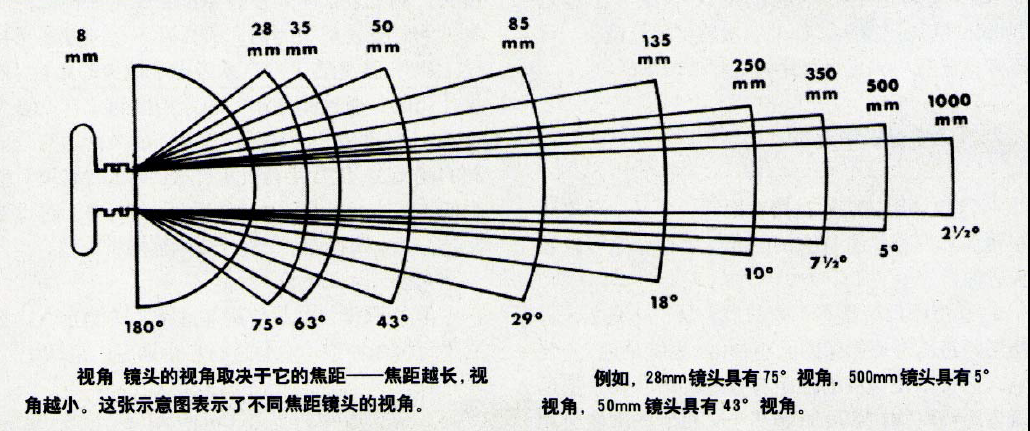
\includegraphics{images/shijiao.png}

\begin{itemize}
\tightlist
\item
  快门速度选择要考虑 物体运动速度 物体运动方向(正面比侧面慢)
\end{itemize}

\subsection{白平衡}\label{ux767dux5e73ux8861}

\begin{itemize}
\tightlist
\item
  色温 不同温度下的光谱 高温偏低波长 低温偏高波长 -1000-2000K 烛光
  -2500-3500K 白炽灯 -3000-4000K 日出 日落 -4000-5000K 荧光灯
  -5000-5500K 闪光灯 -5000-6500K 晴天 -6500-8000K 阴天 -9000-10000K
  阴影或阴霾天
\item
  绿-品红转换 调整人工光源 营造特殊氛围
\item
  使用RAW 通过参考物质还原场景
\item
  自动白平衡判断的是光源光 如果拍摄物体本身偏暖或冷 背景物会偏冷或暖
  就需要手动调节 自动白平衡在有白色物体的画面中更准确
\item
  混合光下自动白平衡会分区对待 手动则为单一色调 可能失真
\end{itemize}

\subsection{自动对焦}\label{ux81eaux52a8ux5bf9ux7126}

\begin{itemize}
\tightlist
\item
  自动对焦传感器 检测对比度 可通过直方图理解 对比度最大对焦最锐

  \begin{itemize}
  \tightlist
  \item
    对焦系统轻微改变对焦距离
  \item
    读取传感器对比度看变化如何
  \item
    根据上步结果调整对焦距离
  \item
    重复上面步骤
  \end{itemize}
\item
  影响因素

  \begin{itemize}
  \tightlist
  \item
    光亮度
  \item
    物体对比度
  \item
    物体动态
  \item
    选择对比度强 低动态 高亮度的物体对焦
  \end{itemize}
\item
  对焦点

  \begin{itemize}
  \tightlist
  \item
    +表示二维对比度检测 更准 在中心
  \item
    -表示一维对比度检测
  \end{itemize}
\item
  自动对焦模式

  \begin{itemize}
  \tightlist
  \item
    连续对焦\&伺服对焦 移动物体对焦 耗电池
  \item
    一次对焦
  \item
    自动对焦辅助光 对比度小的静物比较适合
  \end{itemize}
\item
  对焦位置

  \begin{itemize}
  \tightlist
  \item
    人像对焦眼睛 对比度高
  \item
    偏离中心物体用中心对焦要偏后
  \item
    在条纹场景注意对焦方向
  \end{itemize}
\end{itemize}

\subsection{数码存储}\label{ux6570ux7801ux5b58ux50a8}

\begin{itemize}
\tightlist
\item
  图片用像素存储 像素用RGB存储 RGB用01存储 8位00000000-11111111 256阶
\item
  因为有三个通道 所以有2\^{}(8*3)种颜色 真彩色 32位多一个alpha灰度通道
\item
  人眼可分辨1000w种颜色 24位图像可存储1600w颜色 但更多色阶有利于后期处理
\item
  JPEG跟TIFF文件每个通道只能分别存8位与16位
\end{itemize}

\subsection{锐利度}\label{ux9510ux5229ux5ea6}

\begin{itemize}
\tightlist
\item
  描述图像清晰度 由锐度与分辨率决定

  \begin{itemize}
  \tightlist
  \item
    锐度描述边缘清晰状况
  \item
    分辨率描述相邻单元的区分度 传感器决定
  \end{itemize}
\item
  锐度受颗粒度影响 低颗粒度更柔 高颗粒度更锐
\item
  远近 稳定性均影响锐度 \#\# 图像噪声
\item
  信噪比
\item
  iso 高的噪音高
\item
  类型

  \begin{itemize}
  \tightlist
  \item
    固定模式噪声 长曝光跟温度影响
  \item
    随机噪声 受高iso跟曝光时长影响
  \item
    波段噪声 受传感器影响 跟白平衡有关
  \end{itemize}
\item
  模式

  \begin{itemize}
  \tightlist
  \item
    黑色高白色低 胶片相反
  \item
    曝光不足噪声高 过曝噪声低
  \end{itemize}
\item
  影响因素

  \begin{itemize}
  \tightlist
  \item
    颜色波动
  \item
    亮斑
  \end{itemize}
\item
  频率 高频噪点比低频更易接受 振幅也有影响 可通过RGB直方图标准偏差判断
\item
  通道影响 Bayer排列 -蓝通道噪音最高 -绿通道噪音最低
\item
  像素高底小噪音高 跟电子降噪技术也有关系
\end{itemize}

\subsection{动态范围}\label{ux52a8ux6001ux8303ux56f4}

\begin{itemize}
\tightlist
\item
  最大最小的明暗范围
\item
  强反射与不平衡的直射光场景需要较大的动态范围
\item
  照度与亮度相关 光质决定
\item
  感光元件决定单个像素的容忍度 更大的像素尺寸容忍度更高
\item
  有些相机低ISO是通过抛弃高光部分实现的
\item
  低ISO层次更强
\item
  2的n次方表示几档的光变比
\item
  相机 扫描仪 显示器 打印机的动态范围不一致
\item
  人眼24档的动态范围 相机6-8档左右 红色低蓝色高
\item
  A/D转换 模拟信号转为数字信号 相机使用10-14位A/D转换信号
  但一般就能转化出5-9档
\item
  记录动态范围与展示动态范围是要去别对待的
\end{itemize}

\subsection{传感器尺寸}\label{ux4f20ux611fux5668ux5c3aux5bf8}

\begin{itemize}
\tightlist
\item
  尺寸

  \begin{itemize}
  \tightlist
  \item
    全画幅 35mm胶片尺寸
  \item
    中画幅
  \item
    大画幅
  \item
    APS-C
  \item
    43系统
  \end{itemize}
\item
  切割因子是对角线距离跟35mm对焦线的比值
\item
  镜头的中心部分成像质量好 存在边缘模糊 越大光线使用率越高

  \begin{itemize}
  \tightlist
  \item
    传感器尺寸越大 相同视角焦距越小 越小越广角 边缘成像越差
  \item
    APS-C 23mm焦距相当于35mm 转换倍数1.5
  \item
    传感器越小 需要镜头越轻便
  \item
    传感器越大 镜头越沉 成像质量越好
  \end{itemize}
\item
  景深影响

  \begin{itemize}
  \tightlist
  \item
    传感器越大 景深越浅
  \item
    大传感器需要靠近且长焦 所以景深浅
  \item
    大传感器人像 虚化背景 因为降噪好 拍风景可考虑高ISO 小光圈
  \item
    小传感器风景 景深大
  \end{itemize}
\item
  干涉

  \begin{itemize}
  \tightlist
  \item
    大传感器小光圈干涉少
  \item
    干涉影响分辨率 锐度
  \end{itemize}
\item
  大传感器 像素尺寸大 噪点少 动态范围宽
\item
  同样尺寸 同样噪点 噪点一般为高频 像素越多 高频影响越小 成像越干净
\item
  生产上大块传感器质量要求更高 更贵
\item
  有些镜头配特定传感器
\item
  相同景深 大传感器分辨率不占优势
\item
  同样敏感度 大传感器曝光时间更长
\item
  像素越大 动态范围大 噪点低
\end{itemize}

\subsection{干涉}\label{ux5e72ux6d89}

\begin{itemize}
\tightlist
\item
  艾里斑 2D干涉
\item
  影响分辨率
\item
  颜色影响 波长越小 干扰越小
\item
  同样面积像素越多 干涉越大
\item
  有些像素矩形 所以会向一个方向偏
\item
  间隔中干涉要考虑微棱镜
\item
  干涉并不总是圆形 有时5-8边形
\item
  APS-C在F16会有明显干涉
\item
  小光圈虽然有模糊 但可表现动态模糊与长曝光流水
\item
  分辨率

  \begin{itemize}
  \tightlist
  \item
    绝对分辨率
  \item
    人眼分辨率
  \end{itemize}
\end{itemize}

\subsection{相机vs人眼}\label{ux76f8ux673avsux4ebaux773c}

\begin{itemize}
\tightlist
\item
  可视角度 40-60度 50mm标准镜头
\item
  焦距对比

  \begin{itemize}
  \tightlist
  \item
    眼睛是曲面
  \item
    中间视场比边缘视场细节更多
  \end{itemize}
\item
  分辨率与细节

  \begin{itemize}
  \tightlist
  \item
    人眼60度 分辨率大概500w-1500w
  \item
    人眼识别特定模式 如脸 引起注意
  \item
    不对称 视线下方比上方更引起注意
  \item
    低光下眼睛识别单色 边缘更引起注意
  \item
    人眼在识别某些模式上放大后缺失 跟相机最大不同 反直觉
  \end{itemize}
\item
  敏感度与动态范围

  \begin{itemize}
  \tightlist
  \item
    人眼动态范围一般10-14档
  \item
    相机5-11档
  \item
    灵敏度人眼星空适应后晚上500-1000 白天1
  \item
    低光环境人眼灵敏度好一些
  \end{itemize}
\end{itemize}

\subsection{理解超焦距}\label{ux7406ux89e3ux8d85ux7126ux8ddd}

\begin{itemize}
\tightlist
\item
  在超焦距上对焦可获得从超焦距一半距离到无穷远都清晰的图片
\item
  为了照顾前景中景与背景
\item
  无穷远景深最近的一点
\item
  跟光圈有关(景深)23mm F5.6 5m
\item
  经验对焦在场景的1/3处
\item
  超焦距要注意构图及主题
\item
  注意相机的景深标尺
\end{itemize}

\subsection{单反 vs DC}\label{ux5355ux53cd-vs-dc}

\begin{itemize}
\tightlist
\item
  单反特征

  \begin{itemize}
  \tightlist
  \item
    取景器
  \item
    可换镜 -可用特殊镜头 -画质好 -光圈大
  \item
    传感器
  \end{itemize}
\end{itemize}

\subsection{三脚架}\label{ux4e09ux811aux67b6}

\begin{itemize}
\tightlist
\item
  使用时机 安全快门 焦距的倒数
\item
  全景 合成HDR 动画 合成场景 运动场景
\item
  选购三脚架

  \begin{itemize}
  \tightlist
  \item
    稳定性好
  \item
    重量
  \item
    个人负担
  \item
    支架数
  \item
    最大高度 越矮越稳
  \item
    收缩长度
  \end{itemize}
\item
  云台 vs 滚轴头

  \begin{itemize}
  \tightlist
  \item
    云台可单独控制两个方向
  \item
    滚轴头可一次控制 但不一定稳
  \item
    强度重量比
  \item
    气泡水平仪
  \end{itemize}
\item
  三脚镜头支架
\item
  桌面三脚架 视线越低出图好
\item
  铝 碳纤维三脚架(湿环境用)
\item
  独脚架 运动场景 轴线平面动态模糊
\end{itemize}

\subsection{闪光灯}\label{ux95eaux5149ux706f}

\begin{itemize}
\tightlist
\item
  闪光灯的使用要不留痕迹
\item
  自然光 人造光
\item
  光线决定对比度 软光 硬光
\item
  反光伞反光后柔光 光照度下降
\item
  半透明塑料板 室外没用 室内有用
\item
  过分散的光没有对比度 二维化 相机自带闪光灯有这个问题
\item
  离机闪光灯背对物体效果会好
\item
  闪光支架效果会好 可消除红眼
\item
  辅助闪光灯 消除暗影区 减少对比度 耗电多
\item
  红眼 闪光瞳孔放大 眼底血管尽显 拍照时不要看闪光灯 事先闪光 离远一点
\item
  电子去红眼效果不一定好
\item
  闪光白平衡 矫正闪光带来的白平衡失真
\item
  闪光曝光流程

  \begin{itemize}
  \tightlist
  \item
    自然光与闪光两个曝光 有个预闪光评价自然光
  \item
    闪光时间短于快门 属于曝光阶段中的一部份
  \end{itemize}
\item
  闪光比

  \begin{itemize}
  \tightlist
  \item
    闪光与环境光的比例
  \item
    总光与闪光的比例
  \item
    1:8-1:2 效果好 弱闪光 长曝光 作为补光
  \end{itemize}
\item
  闪光曝光模式

  \begin{itemize}
  \tightlist
  \item
    自动 测光快门低于1/60s启动闪光 快门固定1/60
    闪光强度取决于明暗程度的测光
  \item
    程序 一直开闪光 作为补光 低于1/60s同自动模式
  \item
    光圈优先 闪光比不超过1:1进而延长曝光时间
  \item
    快门优先 最大光圈不够用时启用闪光
  \item
    手动 自己调
  \item
    不能用会闪烁
  \end{itemize}
\item
  闪光曝光补偿

  \begin{itemize}
  \tightlist
  \item
    每一档表示一倍
  \item
    曝光补偿同时影响自然光与闪光
  \item
    保持或改变闪光比要先调闪光曝光补偿 然后计算曝光补偿 1/3一档调整
  \item
    提高闪光比需要增闪光补偿一档 减曝光补偿-1/2--2/3档
  \item
    降低闪光比需要减闪光补偿一档 增曝光补偿1/3-1/2档
  \end{itemize}
\item
  闪光测光

  \begin{itemize}
  \tightlist
  \item
    环境光测量 反射直射不分 婚礼摄影黑白对比高 更容易出错
  \item
    闪光测量 距离影响最大 近亮远暗
  \item
    使用闪光曝光锁定而不是自动曝光
  \item
    不同机器要事先熟悉
  \end{itemize}
\item
  一次二次曝光同步

  \begin{itemize}
  \tightlist
  \item
    处理动态模糊 闪光在前 模糊在后会导致逆向运动
  \item
    二次曝光会增强动态模糊效果
  \end{itemize}
\end{itemize}

\subsection{广角镜的使用}\label{ux5e7fux89d2ux955cux7684ux4f7fux7528}

\begin{itemize}
\tightlist
\item
  概述

  \begin{itemize}
  \tightlist
  \item
    焦距小于35mm 视角大于55
  \item
    超广角 小于20-24mm
  \item
    用于贴近 容纳更多景物
  \end{itemize}
\item
  广角透视

  \begin{itemize}
  \tightlist
  \item
    近大远小
  \item
    变形夸张
  \end{itemize}
\item
  汇聚光线 调整汇聚点在地平线位置 上下会产生不同的倾斜效果
\item
  引导线效果 建筑会夸张高度
\item
  内部或封闭空间 广角包容性
\item
  偏振滤镜 广角用偏振会导致饱和度不均
\item
  广角控光 不均的光环镜 渐变中灰密度镜
\item
  广角镜与景深 与长焦镜景深一致 与使用习惯有关
\item
  使用

  \begin{itemize}
  \tightlist
  \item
    离前景近一些
  \item
    远近景搭配
  \item
    透视效果 引导线
  \item
    边缘失真
  \end{itemize}
\end{itemize}

\subsection{长焦镜的使用}\label{ux957fux7126ux955cux7684ux4f7fux7528}

\begin{itemize}
\tightlist
\item
  概述

  \begin{itemize}
  \tightlist
  \item
    中度长焦70mm 全长焦135mm 视角小于15
  \item
    长焦会压扁 使物体扁平化 距离压缩
  \end{itemize}
\item
  远物近化 测不准原理 小视角画框 强化雾气影响
\item
  浅景深对焦
\item
  长焦需要短曝光来缩短机身摇晃
\end{itemize}

\subsection{移轴镜的使用}\label{ux79fbux8f74ux955cux7684ux4f7fux7528}

\begin{itemize}
\tightlist
\item
  概述

  \begin{itemize}
  \tightlist
  \item
    移轴可使视角变宽 倾斜可改变焦平面位置进而改变景深角度
  \item
    镜头成像圈大 等焦距画质好
  \item
    中度望远镜移轴形成全景 扩大视角
  \item
    移轴镜优化边缘成像质量
  \item
    相比同等光圈焦距 移轴镜更重且成像质量更好
  \end{itemize}
\item
  透视控制

  \begin{itemize}
  \tightlist
  \item
    远点在地平线上 所有线都垂直地面
  \item
    移轴会削弱垂直透视效果 使建筑更高耸 更突出 对焦点在地平线之上
  \item
    普通相机可考虑剪裁或ps
  \item
    移轴镜头优于数码移轴
  \item
    全景拼接上移轴拼接用的更少 传感器小更易移轴拼接
  \item
    视角控制上移轴等效焦距会更小
  \end{itemize}
\item
  景深控制

  \begin{itemize}
  \tightlist
  \item
    沙姆定律 传感器平面 焦平面 影像平面汇聚到一点可得到全面清晰的图像
  \item
    倾斜可使景深成条带状
  \item
    对焦采用试错的方法
  \end{itemize}
\end{itemize}

\subsection{微距镜的使用}\label{ux5faeux8dddux955cux7684ux4f7fux7528}

\begin{itemize}
\tightlist
\item
  放大率 传感器与真实物体大小

  \begin{itemize}
  \tightlist
  \item
    焦距 长焦
  \item
    对焦距离 近
  \item
    严格讲1:1 不严格可放宽到1:10以下
  \item
    传感器越小 像素越高 对小物体放大效果越好
  \end{itemize}
\item
  对焦长度与有效光圈

  \begin{itemize}
  \tightlist
  \item
    越是放大 镜头离传感器就越远
  \item
    进光少 有效光圈越小 景深变大
  \item
    1:1放大比有效光圈缩小两档 曝光时间要延长
  \item
    影响自动对焦与取景
  \end{itemize}
\item
  微距景深

  \begin{itemize}
  \tightlist
  \item
    独立于焦距
  \end{itemize}
\item
  微距衍射

  \begin{itemize}
  \tightlist
  \item
    平衡处理
  \end{itemize}
\item
  工作距离与焦距

  \begin{itemize}
  \tightlist
  \item
    焦距越大 工作距离就可以远
  \item
    不干扰被摄物
  \end{itemize}
\item
  外接管

  \begin{itemize}
  \tightlist
  \item
    用于长焦镜
  \end{itemize}
\item
  闭合滤镜

  \begin{itemize}
  \tightlist
  \item
    用在镜头前 屈光镜
  \end{itemize}
\item
  其他方法

  \begin{itemize}
  \tightlist
  \item
    望远倍率镜
  \item
    波纹管
  \item
    反接镜头环
  \item
    裁剪照片
  \end{itemize}
\end{itemize}

\subsection{棱镜耀斑}\label{ux68f1ux955cux8000ux6591}

\begin{itemize}
\tightlist
\item
  长相 5-8边形 降低对比度
\item
  产生原因 快门形状与棱镜间反光 视角外强光源
\item
  遮光罩

  \begin{itemize}
  \tightlist
  \item
    花瓣型优于圈型 考虑感光元件
  \item
    可调波纹管
  \end{itemize}
\item
  棱镜类型影响

  \begin{itemize}
  \tightlist
  \item
    定焦好于变焦
  \item
    广角镜设计会考虑并添加涂层
  \end{itemize}
\item
  消除方法

  \begin{itemize}
  \tightlist
  \item
    纳入光源
  \item
    引入遮挡物
  \item
    减少镜片数
  \end{itemize}
\end{itemize}

\subsection{镜头MTF、分辨率与对比度}\label{ux955cux5934mtfux5206ux8fa8ux7387ux4e0eux5bf9ux6bd4ux5ea6}

\begin{itemize}
\tightlist
\item
  MTF表示固定分辨率下降随距离镜头中心距离的变化
\item
  线粗细表示对比度大小
\item
  线颜色表示光圈大小
\item
  线型表示散光方向
\item
  一般f8分辨率较好
\item
  不同品牌计算方法不一样
\end{itemize}

\subsection{滤镜}\label{ux6ee4ux955c}

\begin{itemize}
\tightlist
\item
  偏光镜

  \begin{itemize}
  \tightlist
  \item
    减少炫光与反射,天更蓝
  \item
    减光,相当于减少2-3档光圈
  \item
    线性或圆形偏光镜,圆形适用单反,线性不适合
  \item
    广角镜中使用有极化现象
  \item
    日落与彩虹可能因偏光而消失
  \item
    不平玻璃出现偏光彩虹,飞机上出现
  \end{itemize}
\item
  中灰密度镜

  \begin{itemize}
  \tightlist
  \item
    平滑水流
  \item
    强光下大景深
  \item
    减少干涉
  \item
    让流动物体模糊
  \item
    增加动态模糊
  \item
    必要时用,减光很强烈
  \item
    提高动态范围与本地对比度
  \end{itemize}
\item
  渐变中灰密度镜

  \begin{itemize}
  \tightlist
  \item
    使用明暗变化剧烈场景,如日出日落
  \item
    考虑光暗变化的剧烈程度
  \item
    拍摄时考虑位置,强度与透明度
  \end{itemize}
\item
  雾镜或UV镜

  \begin{itemize}
  \tightlist
  \item
    胶片年代UV影响对比度
  \item
    数码时代主要起保护或保值作用
  \end{itemize}
\item
  冷暖镜

  \begin{itemize}
  \tightlist
  \item
    转换白平衡
  \item
    数码时代不太需要
  \end{itemize}
\item
  特技滤光镜-星光镜 多影镜 分像镜 用来区别蓝天白云
\item
  黑白摄影中使用不同的滤光镜可以出现不同的对比效果 例如加强红绿对比
  风光照片用绿色 可以加深蓝色 建筑摄影用红光 可以加深蓝天色调 颜色越深
  蓝色越深 与云彩对比更强 可用偏振镜 雾天也是同样道理 用深色过滤蓝光
\end{itemize}

\subsection{人像摄影}\label{ux4ebaux50cfux6444ux5f71}

\begin{itemize}
\tightlist
\item
  光线参照布景
\item
  镜头高度与眼睛平齐
\item
  布光产生眼下三角区
\item
  鼻下人中影子清晰
\item
  光比3:1或4:1
\item
  反光伞柔和布光
\item
  对眼对焦 光圈f8或更小
\item
  伦勃朗用光法 男性 3/4面部用光 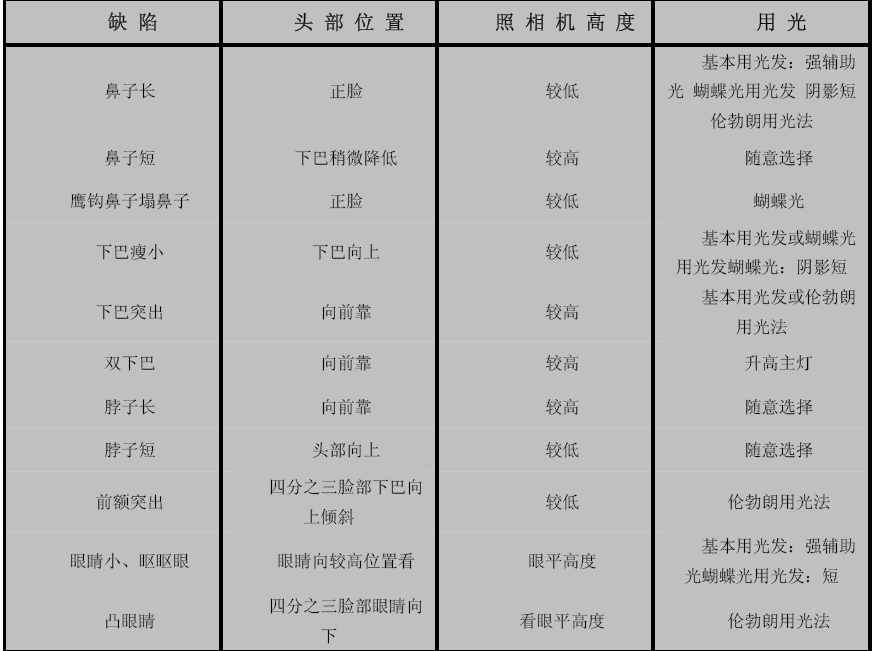
\includegraphics{images/renxiang1.png}
  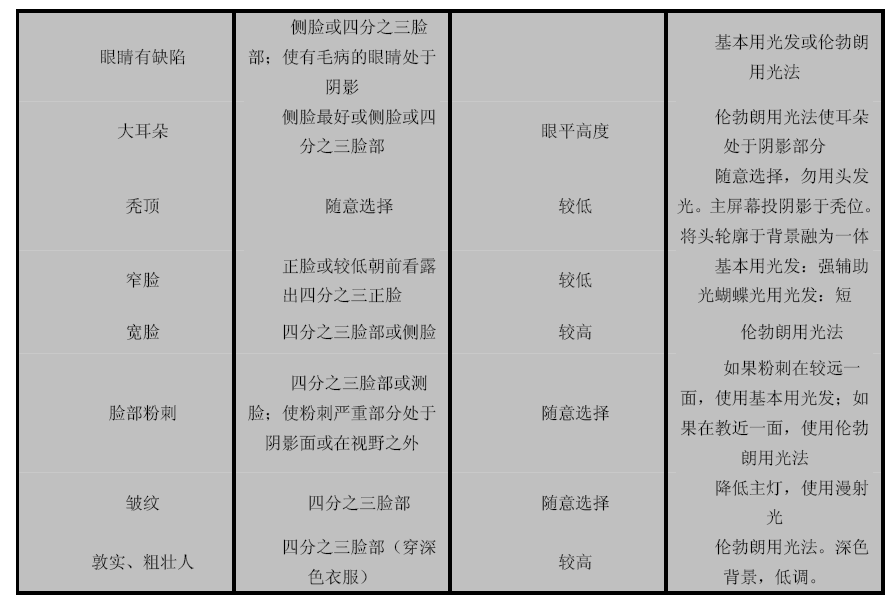
\includegraphics{images/renxiang2.png}
\end{itemize}

\subsection{关心相机与照片}\label{ux5173ux5fc3ux76f8ux673aux4e0eux7167ux7247}

\begin{itemize}
\tightlist
\item
  传感器灰尘
\item
  存储照片 DNG格式?
\item
  光盘5-10年或50-100年
\item
  硬盘磁头可能损坏
\item
  磁带便宜可用,适合大数据量,也会去磁去电
\item
  不断复制会失真,需要RAID保存,校检与修复过程
\item
  保护版权

  \begin{itemize}
  \tightlist
  \item
    隐藏层
  \item
    分片段
  \item
    锁右键
  \item
    用flash展示
  \item
    水印
  \item
    Digimarc
  \item
    数码相框
  \item
    版权协议
  \item
    相似图片搜索
  \end{itemize}
\end{itemize}

\subsection{数码照片后期处理流程概述}\label{ux6570ux7801ux7167ux7247ux540eux671fux5904ux7406ux6d41ux7a0bux6982ux8ff0}

\begin{itemize}
\tightlist
\item
  白平衡

  \begin{itemize}
  \tightlist
  \item
    色温
  \item
    偏色
  \end{itemize}
\item
  曝光补偿与恢复

  \begin{itemize}
  \tightlist
  \item
    图像柱形图
  \item
    远看容易判断曝光
  \item
    极端色调
  \item
    限制 如低光噪点
  \end{itemize}
\item
  噪点还原

  \begin{itemize}
  \tightlist
  \item
    高ISO使用
  \item
    具有专门除噪点软件
  \end{itemize}
\item
  镜头矫正

  \begin{itemize}
  \tightlist
  \item
    光晕
  \item
    变形
  \item
    色散
  \end{itemize}
\item
  细节

  \begin{itemize}
  \tightlist
  \item
    锐化
  \item
    局部对比度
  \end{itemize}
\item
  对比度

  \begin{itemize}
  \tightlist
  \item
    强光会降低对比度
  \item
    过高会导致不真实,颜色过饱和
  \end{itemize}
\item
  矫正剪切

  \begin{itemize}
  \tightlist
  \item
    拉伸
  \item
    剪切
  \end{itemize}
\item
  精细化

  \begin{itemize}
  \tightlist
  \item
    色彩
  \item
    选择增强
  \end{itemize}
\item
  缩放

  \begin{itemize}
  \tightlist
  \item
    不同用途不同缩放
  \item
    保留原始样本
  \end{itemize}
\item
  外放增强

  \begin{itemize}
  \tightlist
  \item
    选择性优化输出图片
  \end{itemize}
\item
  其他

  \begin{itemize}
  \tightlist
  \item
    存储
  \item
    显示器矫正
  \end{itemize}
\item
  gimp colors-levels
  手动寻找白点,灰点,黑点或自动,可以按照各个通道调节色阶分布,使三原色向中间靠拢,整体就不会显得偏色

  \begin{itemize}
  \tightlist
  \item
    gimp colors-color balance 调节颜色平衡
  \item
    gimp Color Temperature Plugin 调节色温值
  \item
    \href{http://spencerrf.blogspot.com/2009/06/gimp_08.html}{网络教程}
  \end{itemize}
\end{itemize}

\subsection{构图}\label{ux6784ux56fe}

\begin{itemize}
\tightlist
\item
  1/3构图 中心构图 表达主题
\item
  用环境构成画框
\item
  用光可指引主体
\item
  注意景深调节
\end{itemize}

\subsection{用光}\label{ux7528ux5149}

\begin{itemize}
\item
  三要素 明暗 方向 色彩
\item
  正面 光源看镜头 清晨 傍晚 正午 无层次 平光
  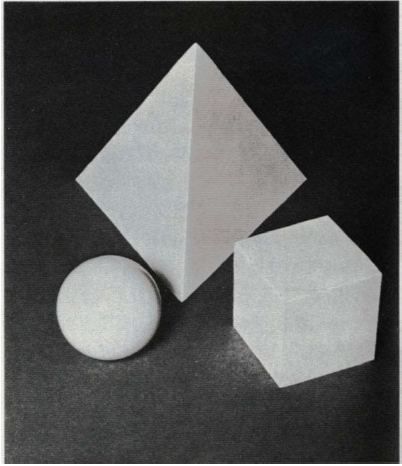
\includegraphics{images/front.png}
  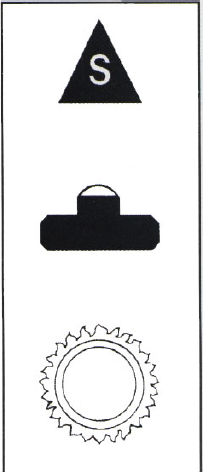
\includegraphics{images/posfront.png}
\item
  侧面 45 上午九十点 下午三四点 用于人像摄影 称为自然光 有立体效果
  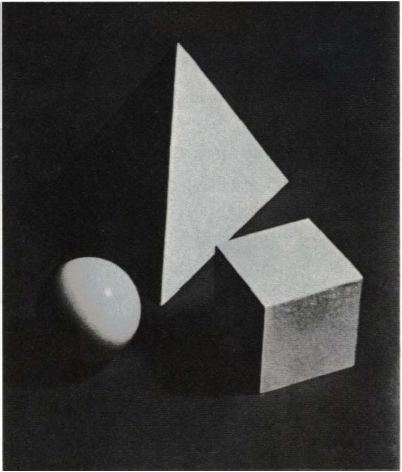
\includegraphics{images/side.png} 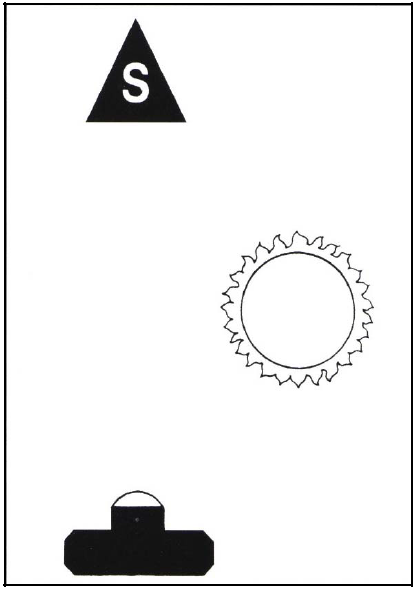
\includegraphics{images/posside.png}
\item
  90侧光 结构光 用来表达细节 强调对比 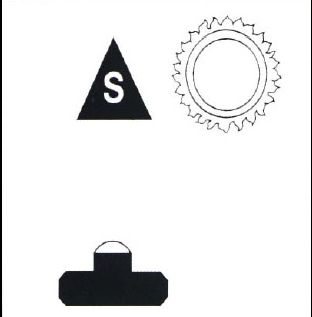
\includegraphics{images/right.png}
\item
  逆光 轮廓光 剪影 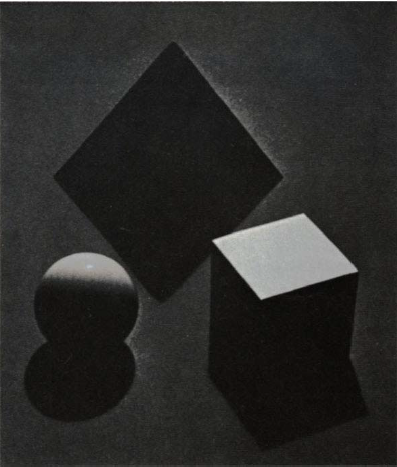
\includegraphics{images/back.png}
  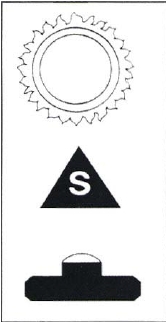
\includegraphics{images/backpos.png}
\item
  现场光对亮光处测光 然后缩小光圈 可以只保留亮光细节来保证主题简洁
\item
  人造光-无缝背景纸 泛光灯 聚光灯 反光伞可以让光更柔和
  黑白受色温影响不大
\end{itemize}

\subsection{布光步骤}\label{ux5e03ux5149ux6b65ux9aa4}

\begin{itemize}
\tightlist
\item
  先放置主灯 45度 辅灯补充阴影部分光
  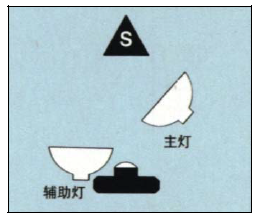
\includegraphics{images/mainlight.png}
\item
  添置背景灯形成区分度 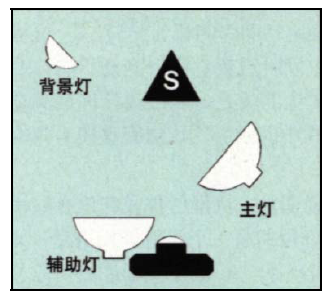
\includegraphics{images/backgroundlight.png}
\item
  肖像主辅光灯 4:1
\end{itemize}

\subsection{胶片}\label{ux80f6ux7247}

\begin{itemize}
\tightlist
\item
  iso感光量成比例放大
\item
  光敏物质都是银盐
\item
  彩色照片分为反转片与负片 前者需要二次曝光 颜色与原来一致
  白平衡要事先调节(日光与钨光灯)后者正常使用即可 白平衡可冲洗时调整
\item
  感光度、颗粒感与反差是胶片选择首要考虑的东西
\item
  对被摄体进行近距离测光
\item
  必要时使用替代读数
\item
  高反差范围需要考虑高光不要溢出 尽可能的保留细节
\item
  摇黑卡或补光都可以考虑 后期可以让细节显示出来
\item
  考虑包围曝光来处理一些高反差的场景
\item
  黑白
  卤化银感光后团聚形成潜影,用显影液可以将卤化银转为金属银后停显,然后用定影液洗掉相应未感光卤化银,流水冲干净后就可以出负片了,投影负片在相纸上就有照片了
\item
  彩色
  用三原色分为三层,每层银盐感光后会有彩色染料偶联,洗照片的时候显色,反转片要二次曝光,胶片就是原色,曝光宽容度小,一般负片是相反颜色,可制作正片
\item
  安全灯 黑白相纸对部分红光不敏感
\end{itemize}

\subsection{训练}\label{ux8badux7ec3}

\begin{itemize}
\item
  训练1、全景深练习
    被摄体:一般风景、花卉、城市建筑等冲击力较强的景物。要
  求:画面全部实焦。   建 议:首先使用广角镜头:24MM---35MM拍摄, 光
  圈:F11---16,光圈优先AE模式。
\item
  训练2、单体对焦练习   要 求:只把焦点对在主要被摄体上,浅景深。   建
  议:中望远镜头:85MM以上,光圈F5.6或更大。光圈优先AE模式。
\item
  训练3、定格练习
    被摄体:体育运动项目、行走着的汽车、火车,流动着的水,瀑布等。   要
  求:将激烈运动着的被摄体的瞬间动作或瞬间表情记录下来。   建
  议:高速快门1/1000秒以上、快门速度优先AE模式。
\item
  训练4、动感练习   被摄体:体育运动项目、动态的人、流动着的水,瀑布等。
    要 求:
  运动员和动态人的身体的一部分虚化或动体实背景虚。流动着的水,瀑布等有流线感。
    建
  议:慢速快门1/15秒-11秒。先从1/30秒开始练习,然后1/15、1/8、1/4、1/2、1秒逐段练习。使用三脚架。
\item
  训练5、取景练习   要
  求:突出主题,画面简练,能传达出被摄场景的气氛*此项训练是构图训练的基矗
  。.   建 议:望远镜头,大光圈。
\item
  训练6、特写练习   被摄体:花卉、静物、昆虫等。   要 求:
  被摄体占画面的比例尽量大,突出被摄体的形状和有趣的部分,高清晰度。
    建 议:
  使用微距镜头或微距功能及近摄接圈,最短摄影距离,镜头与被摄体保持平行。使用三脚架及快门线。
\item
  训练7、各种焦距镜头(镜头各焦段)的使用练习
\end{itemize}

  利用各种焦距镜头(镜头各焦段)进行拍摄练习,借此了解镜头各个焦距的特点,理解画角及透视关系,活用各焦距段的不同景深。
  标准镜头: 焦距50MM左右的镜头------极其自然,没有夸张。   广角镜头:
焦距35MM以下的镜头------强调远近感。
  中望远镜头:焦距为85MM~135MM的镜头------与人眼最接近的透视(远近)感,能正确体现被摄体的形状,
Q YF多用于人像摄影。
  望远镜头:焦距为200MM以上的镜头------很少远近感,有压缩效果。(易抖动,尽量使用三脚架)

\begin{itemize}
\item
  练习8、横、纵位构图   被摄体:景物、山河、建筑、人物等.   要 求:
  用横位构图表现稳定感和宽阔感,用纵位构图表现纵深
  感和高度感,画面不能有无用的空间.   建
  议:1、对同一被摄体分别用横、纵位构图法拍摄,比较作品的不同感受.
    2、横位构图表现安定感时使用标准焦点以上的镜头,表现宽阔感时使用广角镜头
    3、纵位构图表现纵深感与高度感时使用广角镜头,注意画面中近景与远景的位置配置.
  构图时应特别注意水平与垂直,使用三脚架.
\item
  练习9、三角形构图   被摄体:三角形或类似三角形的景物,建筑,人物造型等.
    要 求:
  利用三角形在画面中不同的位置配置,表现稳定感、跃动感、高度感和宽阔感.
    建
  议:1、画面中有容易识别的三角形造型,三角形构成的复数物体焦点要实,要有平衡感.
    2、高楼大厦和道路等高大细长的景物时使用20MM以下的广角镜头
    3、使用景深预测功能
\item
  练习10、对称形构图
    被摄体:所有具有对称构图性质的景物、人物造型、建筑等.   要
  求:利用上下左右对称构图,表现稳定感和超现实意境.   建
  议:1、选择优美的对称形,对称形的两边焦点都要实,每个对称形表现要明显.
    2、尽量使用标准焦点以上的镜头,使用光角镜头时要注意相机与被摄体保持平行.
    3、拍摄岸边与水中的对称构图景物时使用偏光镜
    4、求全景深不得不用小光圈时使用三脚架.
\item
  练习11、垂直、水平构图   被摄体:风景、建筑等   要
  求:画面中表现由多条平行或垂直线条构成的单纯美.   建
  议:画面构成的线条要保持水平或垂直,线条要美,
  水平或垂直线条造型要布满全画面. 使用三脚架 。
\item
  练习12、S形、斜线构图
    被摄提:具有S形或斜线构成的道路、河流、山峦、都市内的桥梁和道路等.
    要
  求:用S形表现纵深感,用斜线表现外展的广阔感和动感.S形要通达画面的两端,中途断了的话前面要有空间构成.
    建
  议:S形及斜线的配置要有平衡感,要仔细感觉作品是否有纵深感和广阔感,被摄体是否清晰.
  \}主题要突出.
\item
  练习13、黄金分割法构图   被摄题:任何均可   要
  求:被表现的主体要处在分割点、线上或附近,构图要平衡.被摄体要突出.
  画面中不能有多余的部分存在.   建
  议:首先按自己的想法构图,然后再活用黄金分割法。
\item
  练习14、昼间闪光灯曝光补偿
    被摄体:人物、花卉、宠物、小范围自然景色、静物等近距离小范围景物。
\end{itemize}

  要求:当以上被摄体处于逆光、侧逆光并周围光线强于被摄体时或被摄体处于昼间阴暗处时使用。
建议:1、用闪光灯同步速度测光(平均测光)取得光圈值,然后用闪光灯的指数除以光圈值得到拍摄距离,就能得到曝光准确的照片。
瞬例如:相机的闪光同步是1/125秒,用相机的自动测光得到的F值16,闪光灯的指数(GN)是40,即40÷16(F)=2.5M,这时的拍摄距离为2.5米。
已知闪光指数(GN)和距离求光圈(F)时用闪光灯指数除以距离求得光圈(F)。
即:GN÷距离=F。

\begin{itemize}
\tightlist
\item
  练习15、利用闪光灯体现作品的立体感
    被摄体:人物、花卉、、宠物、静物等。
\end{itemize}

  要求:使用外置闪光灯并利用连线使闪光灯离开相机,从斜上方或背后投光制造立体感,也可以投到天花板或利用反光板制造折射的柔光,具体投光方法与方向按自己意图具体安排。但是要尽量避免重阴影。

  建
议:可能的情况下尽量尝试各种投光方式及曝光补偿所制造出来的立体感觉。

\begin{itemize}
\tightlist
\item
  练习16、室内及夜晚灯光摄影
    被摄体:室内灯光下的集会以及城市灯光夜景等。
    要求:利用色温在室内及夜灯下制造肉眼见不到的独特(泛红)氛围。
\end{itemize}

  建议:画面内的光线布置尽量均匀,镜头附近最好没有强光源并不能有强光射进镜头,拍静物时使用三脚架,抓拍时最好使用ISO400的胶卷。如果希望得到忠实于原色的作品,使用80A滤镜矫正色温。曝光不能有过。

  参考:色温:白日晴天=5500K,白日阴天=6500K,早晚=4500K,一般灯光=2800K。

\begin{itemize}
\tightlist
\item
  练习17、朝阳、夕阳、夜景
    被摄体:朝阳、夕阳下的山峦、海岸线、自然风光及夜景。
    要求:要充分体现朝夕的氛围,再现朝夕夜景的绚丽景色,不能有多余的物体进入画面,最好没有晕光。
\end{itemize}

  建议:使用手动,基本上光圈为F8~11左右,AE光圈优先,远景时焦点调到无限远,10M以内对点光源等最容易看清楚的物体上对蕉,使用三脚架,可以考虑多次曝光。

\begin{itemize}
\item
  练习18、白色物体   被摄体:雪景、白色沙滩、白色花卉等白色物体。
    要求:清晰再现白色物体的质感与色调。
    建议:根据实测曝光量适当曝光补偿,补偿量根据白色物体占画面的比例和你要表现作品的意图一般为0.5~1.5EV之间,画面中黑白物体相间时根据各占比例调整。
\item
  练习19、逆光(透射光)的运用
    被摄体:光线从背后照射的人物、风景、花卉、静物及抓拍等   要
  求:充分利用逆光的特点制造透明感和立体感.注意被摄体与背景的亮度平衡及不能有创作意图以外的光晕产生.
\end{itemize}

  建 议:使用曝光补偿以及反光板.
曝光补偿量有+0.5、+1.0、+1.5、+2.0EV等,补偿越大,被摄主题越亮,如果把握不好曝光补偿量,可以分段补偿各拍一张以上以保证拍摄成功。

\begin{itemize}
\tightlist
\item
  练习20、侧光的运用
    被摄体:与此种光线有关的人物、风景、花卉、植物、宠物以及抓拍.
    要
  求:充分活用阴影的效果,使画面的氛围符合自己的拍摄意图,通过练习提高对光的敏感性.
\end{itemize}

  建
议:拍摄时从顺光、侧光、斜策光、半逆光、逆光的顺序去观察被摄体,并注意侧光与逆光所制造出的物体立体感之差别.如利用强侧光可塑造男人的刚毅和弱侧光可营造女人的温柔等.使用遮光罩。

\begin{itemize}
\item
  练习21、林中点光与泻光的运用
    被摄体:具有泻光特点的林中、阴天下的风景如山峦、江和湖海的水面等
    要 求:充分利用点、泻光的特点营造出印象深刻和感动人的氛围.   建
  议:注意光比范围及曝光量的掌握,明暗差要适当,用点测光方式测得明处与暗处的曝光量后取中间值进行最后的曝光。
\item
  练习22、极端曝光的应用
    被摄体:想要高调表现(阴影淡的)或低调表现(反差大的)的一切被摄体材
    要
  求:摄影意图以及主题要鲜明,要考虑采用高调或低调的必要性,被摄体的所具有的氛围要协调.
    建
  议:高调的曝光补偿从0~+2.0,低调的曝光补偿从0~-2.0,通过分段曝光,掌握在各种条件下的曝光补偿所带来的效果。
\item
  练习23、光的轨迹   被摄体:夜间流动的车、船、星空、焰火等.   要
  求:流畅地表现光的流动,光的流线色彩、形状、大小与周围的气氛要协调,
  曝光要适当.
\end{itemize}

  建
议:利用平均测光与中央部分重点测光模式。也可以把光圈设定为F4或F5.6,
曝光为30秒至2分钟(可用B门)。焰火一般使用ISO100胶片,光圈在F5.6~F11之间.星空的曝光时间最长可到1~2小时。以上均使三脚架。

\begin{itemize}
\tightlist
\item
  练习24、有灯光照明的物体
    被摄体:都市内夜间被灯光照亮的建筑以及植物等   要
  求:取景角度要体现被摄体的魅力,选择能够充分表现气氛的曝光,画面中主体的所占比例要适当。
\end{itemize}

  建
议:使用三脚架、快门线,使用手动模式,B门或T门,使用曝光补偿+0.5---1.5EV。注意构图时画面中最亮部分与最暗部分,避免亮度相差悬殊,长时间曝光时注意倒易失律问题。使用广角镜头!

\begin{itemize}
\tightlist
\item
  练习25、26、27、28、29、30
    分别以红色、蓝色、黄色、绿色、白色、黑色为主要特征的被摄体做表现主题的练习。
\end{itemize}

  被摄体:具有以上颜色的各类物体及颜色着装的人物、花卉等。   要
求:要表现出以上个种颜色的鲜明特征,把握好色调、明亮度、饱和度这色彩的三要素。
  建
议:注意冷暖色的表现,可能的话使用滤色镜,使用包围式摄影法体验曝光补偿对色彩表现的作于用。

\begin{itemize}
\item
  练习31、表现水的透明感   被摄体:与水有关的任何物体。   要
  求:在表现水透明感的同时注意作品的整体表现。   建
  议:注意水面的光反射,使用PL镜,使用是旋转PL镜找到最佳表现。
\item
  练习32、色彩对比
    被摄体:各种颜色掺杂形成对比的田野、公园、建筑群等。   要
  求:利用色彩对比增强作品的感染力。   建
  议:不要使太多的色彩进入画面,形成对比色彩的亮度差越大对比度越强,明亮色与形成对比的暗色容易醒目,同一颜色的实焦点处与虚焦点处可以形成对比。
\item
  练习33、黑白摄影   被摄体:任何物体、人物等。   要
  求:主题与背景的关系性,理解黑白摄影作品的特性。   建
  议:有必要了解彩色变成黑白后的具体变化,既把红色当做浓黑、黄色当做灰色考虑等,
  6Y R并了解与灰阶的关系。
\item
  练习34、单色调的表现
    被摄体:大自然中的群生植物,大面积单色花卉,色调统一的室内房厅等。
    要 求:有效使用统一的色调,构图平衡,充分掌握色彩的浓淡度。   建
  议:注意色彩的饱和度,使画面内的色彩表现有张有弛,使用色温滤镜。
\item
  练习35、动感的表现   被摄体:体育运动、动物、纪念活动、花草、河流等。
    要
  求:充分记录并表现运动的物体或人,表现出运动着的力量感和动态美,合理构图,掌握适合被摄场景的快门和按快门的时机。
\end{itemize}

  建
议:如果条件允许,尽量使用快门优先模式,定格高速运动时使用快门速度为1/500-1/1000秒,表现流动感时使用1/15-1/4秒,追拍时可使用1/15或1/30秒。

\begin{itemize}
\tightlist
\item
  练习36、临场感的表现
    被摄体:火灾及事故现场,祭祀活动,仪式,自然气象状况等。   要
  求:尽量表现临场感,使人身临其境。即使是较平凡的被摄体,也要利用技术与器材制造出临场感。
\end{itemize}

  建
议:尽量接近被摄体使用超广角或望远镜头,光圈使用F11、F16、F22求大景深。表现自然气象状况如台风、大雨、雾、急流时使用三脚架,快门1/8、1/4、1/2秒优先,并可使用包围式拍摄法。

\begin{itemize}
\item
  练习37、寂静感的表现   被摄体:自然风光。   要
  求:摄影者自身要宁静安稳,选择最佳的拍摄时间和天气,选择稳定简洁且容易传达静感的构图方式。
    建
  议:拍摄时间最好在黎明、傍晚、明月夜、雨天、雾、雪天等。选择对称、三角形等增加寂静感,构图要横平竖直,不能有倾斜以强调集中感和稳定感。使用三脚架。
\item
  练习38、感情的表现
    被摄体:人、动物的脸部特写与身体(动作的瞬间抓拍)。   要
  求:掌握最佳快门时机,做到与被摄人或动物心感相通,除脸部外也要注意其他肢体的表现与主题相吻合,注意构图的各个细节。
\end{itemize}

  建
议:先从身边的人特别是小孩和宠物开始练习,平时多多注意他们(它们)的喜怒哀乐,并找出有趣的特点,然后利用望远镜头在被摄人或动物不注意的时候抓拍。开始练习时尽量利用自动模式

\section{字体研究}\label{ux5b57ux4f53ux7814ux7a76}

来自《字体的故事》

\subsection{font}\label{font}

\begin{itemize}
\tightlist
\item
  旧称fount
\item
  typeface的子集
\item
  法语fonte 也就是「铸造」 指铅铸的字母
\item
  fund(数量)而来,也就是指一定数量的活字
\end{itemize}

\subsection{衬线字体}\label{ux886cux7ebfux5b57ux4f53}

\begin{itemize}
\tightlist
\item
  1977年 SanSerriffe 恶作剧
\item
  113年 图拉真石柱
\end{itemize}

\subsection{衬线字体}\label{ux886cux7ebfux5b57ux4f53-1}

\begin{itemize}
\tightlist
\item
  1816年 caslon Egyptian 用于海报
\item
  Akidenz Grotesk 德国 新无衬线字体
\item
  Univers Helvetica 瑞士 后现代
\end{itemize}

\subsection{字型分类}\label{ux5b57ux578bux5206ux7c7b}

\begin{itemize}
\tightlist
\item
  Vox系统 9类
\item
  构造

  \begin{itemize}
  \tightlist
  \item
    字怀 counter 封闭或半封闭空间 o b n
  \item
    字碗 bowl 字母弯曲 g b
  \item
    主干 stem
  \end{itemize}
\item
  弯衬线 直衬线 斜衬线
\item
  基线 x高度
\item
  升部 中线向上
\item
  降部 基线向下
\item
  连字 ligature fi ae 等
\end{itemize}

\subsection{字体大小}\label{ux5b57ux4f53ux5927ux5c0f}

-报纸书籍 8-12够用 - 1英寸 72点 - 1点 0.351mm 或 0.376mm - pica
12点1派卡

\subsection{Letraset 干转印纸}\label{letraset-ux5e72ux8f6cux5370ux7eb8}

\begin{itemize}
\tightlist
\item
  刮刮纸
\item
  取代金属热转印
\item
  被计算机取代
\end{itemize}

\subsection{字体心理学}\label{ux5b57ux4f53ux5fc3ux7406ux5b66}

\begin{itemize}
\tightlist
\item
  别用Courier字体,除非想要看起来像个书呆子。它是图书馆馆员和数据公司的最爱。
\item
  使用Univers这样无衬线字体的人倾向于重视他们的安全和匿名身份。
\item
  comic sans 哗众取宠的人用的,有更多个性表达
\item
  觉得自己可爱可以用Jhelley字体
\item
  「如果你是在写那些将要改变人生的书信,确保字体要小,保持简约。此处少绝对就是多。大字体会揭示出一定的不安全感。
\item
  人们会觉得字母O又大又圆而且还带有尾巴的字体更有人性也更友善,或许是因为这种字体看起来像是在模拟人的面孔。带有更多直线和交角的字体则具有严厉、技术、冷酷的言外之意\ldots\ldots 用心理学的术语来讲,它们是情感上被压抑的,或者说,肛门滞留的
\end{itemize}

\subsection{易认性与易读性}\label{ux6613ux8ba4ux6027ux4e0eux6613ux8bfbux6027}

\begin{itemize}
\tightlist
\item
  cooper black 易于辨认但不易于小尺寸阅读
\item
  时装型字体
\item
  字偶间距 kern 调整相邻字母不被影响
\item
  易读性依赖品味与习惯
\item
  Albertus 易读字体
\end{itemize}

\subsection{\&}\label{section}

\begin{itemize}
\tightlist
\item
  et的组合缩写
\item
  ampersand = et, per se and
\item
  Coming Together 活动
\end{itemize}

\subsection{例句}\label{ux4f8bux53e5}

\begin{itemize}
\tightlist
\item
  The quick brown fox jumps over the lazy dog.
\item
  Quick wafting zephyrs vex bold Jim.
\item
  Quick wafting zephyrs vex bold Jim.
\item
  Zany eskimo craves fixed job with quilting party.
\item
  Playing jazz vibe chords quickly exites my wife.
\item
  Mix Zapf withVeljovic and get quirky Beziers.
\item
  Typography isknown for two-dimensional architecture and requires extra
  zeal withinevery job.
\item
  Hamburgers \textbar{} Hamburgerfont
\item
  LoremIpsum Dolor Letraset字体贴纸
\item
  Handgloves 目前最常用
\end{itemize}

\subsection{常见字体}\label{ux5e38ux89c1ux5b57ux4f53}

\textbf{Textura}

\begin{itemize}
\tightlist
\item
  古腾堡使用
\item
  第一款字体
\item
  第一套圣经现存48本 12本无缺
\item
  更为流畅的威尼斯体打破了这种哥特式字体
\end{itemize}

\textbf{Helvetica}

\begin{itemize}
\tightlist
\item
  1957年诞生
\item
  简洁 现代 无处不在
\end{itemize}

\textbf{Baskerville}

\begin{itemize}
\tightlist
\item
  Q比较特殊
\item
  活字天才
\item
  夫人 MrsEave字体
\end{itemize}

\textbf{Gill sans}

\begin{itemize}
\tightlist
\item
  经典无衬线字
\item
  设计师乱伦
\item
  正文字体
\end{itemize}

\textbf{Comic Sans}

\begin{itemize}
\tightlist
\item
  源于漫画
\item
  类似幼圆
\item
  抵制运动
\item
  不像字体的字体
\end{itemize}

\textbf{Futura vs Verdana}

\begin{itemize}
\tightlist
\item
  宜家门
\item
  Verdana作者是少数靠字体发家的人
\item
  德国人推出的字体
\end{itemize}

\textbf{Johnston Sans}

\begin{itemize}
\tightlist
\item
  最早现代无衬线字体
\item
  出现在中地铁
\end{itemize}

\textbf{Frutiger}

\begin{itemize}
\tightlist
\item
  更有人味的字体
\item
  Univers续作
\end{itemize}

\textbf{Gotham}

\begin{itemize}
\tightlist
\item
  影响选举
\item
  质朴稳定
\end{itemize}

\textbf{Arial}

\begin{itemize}
\tightlist
\item
  仿 Helvetica
\item
  更圆滑
\item
  来自微软
\item
  因疑似抄袭而受质疑与鄙视
\end{itemize}

\textbf{Sabon}

\begin{itemize}
\tightlist
\item
  书籍最常用
\item
  来自德国
\end{itemize}

\textbf{Vendome}

\begin{itemize}
\tightlist
\item
  触觉 雕塑感
\item
  华丽
\item
  来自法国
\end{itemize}

\textbf{Doves}

\begin{itemize}
\tightlist
\item
  用来印刷圣经
\item
  失传 扔到泰晤士河了
\end{itemize}

\subsection{最差字体}\label{ux6700ux5deeux5b57ux4f53}

\textbf{Ecofont}

\begin{itemize}
\tightlist
\item
  省墨
\item
  网眼
\item
  不影响识别
\end{itemize}

\textbf{Souvenir}

\begin{itemize}
\tightlist
\item
  设计师最恨
\item
  真男人不用
\item
  1914年制作
\end{itemize}

\textbf{Gill Sans Light Shadowed}

\begin{itemize}
\tightlist
\item
  让人头昏眼花
\item
  三维效果
\item
  埃舍尔版画
\end{itemize}

\textbf{Brush Script}

\begin{itemize}
\tightlist
\item
  仿手写
\item
  单调 非企业风格
\end{itemize}

\textbf{papyrus}

\begin{itemize}
\tightlist
\item
  卡梅隆在阿凡达里使用
\item
  滥用
\item
  贺卡专用
\item
  埃及纸草书
\end{itemize}

\textbf{Neuland inline}

\begin{itemize}
\tightlist
\item
  非洲风格
\item
  粗厚有棱角
\item
  主题公园体
\end{itemize}

\textbf{Ransom Note}

\begin{itemize}
\tightlist
\item
  拼凑风格
\item
  喜剧风格
\item
  胶水恐吓感
\end{itemize}

\textbf{2012奥运会字体}

\begin{itemize}
\tightlist
\item
  做工粗劣
\item
  街头涂鸦
\end{itemize}

\subsection{中文字体}\label{ux4e2dux6587ux5b57ux4f53}

\begin{itemize}
\tightlist
\item
  思源黑体
\item
  思源宋体
\item
  文泉译
\item
  可购买字体商用,否则宋体、楷体、黑体、隶书等可用
\end{itemize}

\section{装机必备}\label{ux88c5ux673aux5fc5ux5907}

现在有了云账号,更新硬件后迁移软件环境已经很容易了,但折腾软件的心情也不多了,很多就直接用系统自带的。不过鉴于畏惧互联网大公司对隐私的滥用,也会做些可能没啥用的小众选择。现在大部分原来需要单独装软件的要么用在线版,要么直接手机上应用解决,电脑基本就是写东西处理数据用,纯生产环境。

浏览器用火狐,日常写东西用 typora 或 sublime text,编程用R,IDE用
RStudio,网络分析用cytoscape,文献管理 zotero,密码管理1p,虚拟容器
docker,FTP 用 filezilla,远程桌面用 microsoft remote
desktop,开会zoom,无线网用 boingo
wifinder,rss用reeder,其余的都是系统自带。

\section{宠物筛选法}\label{ux5ba0ux7269ux7b5bux9009ux6cd5}

\section{博物馆物语}\label{ux535aux7269ux9986ux7269ux8bed}

刚开始旅游是具有打卡式仪式感的,带点对别人炫耀的小心思,好像必须去一些地方拍些照片留个念想。现在旅游更多是照顾自己感受了,所剩无几的仪式感也是完成自己的某种想法,到这个时候就没有太多不看亏了的想法了,毕竟大多数时候看了看不懂也是亏。有些风景要在最好的年纪以最好的心态去看才有那独一份的体会,错过了也就是错过了,没有可遗憾的,太多人执着于拿不起到拿得起的个人成长路线,却一直因为纠结他人的评价而放不下,殊不知体会这东西是最没必要人人一样的,给自己留点不用分享的空间也是正常。

出行要是看自然景观还是很累的,人文景观没有积淀也就是走马观花,从满足好奇心角度博物馆算是最方便的了。细想下来也去过几十家博物馆了,每到一个新的城市,工作之余自然就是游玩下当地景观,最近的自然就是博物馆。我这种``独夫''式游客比较排斥团体活动,自己懒的当领导操心又对别人瞎指挥与乱规划严重不满,索性独来独往的,因此基本不会去报团,又因为懒所以对博物馆特别有兴趣。博物馆通常有较为系统的主题展,比较大的博物馆则兼容并包啥都有值得一去再去,在北京时除了带朋友去故宫博物院就是去国博了,前后也得有近十次了,另外各省的省级博物馆都值得一游,其余的就不用看了,类似观复这样的太少。加拿大多伦多的皇家博物馆、安省美术馆也重访过,东西很全就是比较凌乱。渥太华的国家美术馆各种艺术流派也非常齐全。蒙特利尔的蒙特利尔美术馆是目前我认为最系统的展馆,了解西方美术各种风格看这一个馆就够了。亚特兰大的高等艺术博物馆也很不错,不愧为美国南方首都。波士顿的波士顿美术馆也很大,不过理工科应该去的是MIT的博物馆,那边更有意思。纽约大都会我去了十次还是每次都有新发现,自然历史博物馆去了两次但学到的东西最多,现代艺术博物馆跟惠特尼美术馆的特展都很不错,不过我最喜欢的是库珀·休伊特史密森尼设计博物馆,展品最精致的则是弗里克收藏馆,跟建筑融合最好的是纽约市博物馆与大都会修道院博物馆。而出了曼哈顿最近的综合性博物馆是布鲁克林博物馆,要是没有大都会看这个也非常好。

从经济上说国内就老老实实买票吧,其实按国际价格也算不上贵,不知道人大门口现在还有没有办假学生证的,但咱就凭这张老脸就跟学生绝缘了。国外博物馆跟国内比肯定是贵的,但如果是本地居民是可以通过当地图书馆拿到免费的票的,纽约则是NYCID一卡通。不过我利用最多的则是开放日,这些博物馆每周或每个月都有一天的晚上是可以免费或自付费参观的,自付费我一律5美元。另外就是很多票是不包括特展的,一般大博物馆都有常设展与特展,常设展你什么时候来都能看到,特展则是在某个时间内巡展,会额外收费但我觉得挺值的,如果时间富裕就一定会看特展,很多特展按主题收集的藏品来自多个博物馆,可以很系统了解某一个主题。我感觉最坑的一次就是在加拿大看过的一个特展后来又到纽约大都会展出而大都会特展并不额外收费。有些博物馆本身就是主题,例如多伦多的巴别鞋博物馆还有美国的一些航母博物馆(本身就是退役航母)及类似摩根图书馆、可口可乐博物馆还有铸币博物馆啥的。有些博物馆则基本没有常设展,主要靠特展,这种就得查好了再去,常去常新,例如纽约当代博物馆,其实惠特尼的特展也占大部分。还有些地方名字不像博物馆但也有展出,例如日本协会瑞士协会啥的,是对应国家为宣传本国文化设立在海外的场馆,通常有其他职能。

说到底你要是当地居民,玩图书馆的心态跟游客区别还是很大的。当你知道可以反复来时间上心态上就更方便欣赏,而旅游则不得不考虑时间成本,总想看最值得看的,其实能进博物馆都值得看,因为值不值其实应该你说了算而不是旅游指南说了算,但办会员通常是不太值的。你来了,你看到了,你感受到了,这都是你的东西,不需要分享与指导别人,所有人天生都有感受美的能力,去迎合别人或所谓专家的口味非常可笑,美丑与真假对错是两回事,真纠结真假你应该来做科研,纠结对错去搞伦理,去博物馆就是开拓眼界放松身心的,要是累个半死身心俱疲真没必要。当你走过某个展品突然被展品本身吸引时是逛图书馆的最高光时刻,这无关这件展品背后的故事与技术背景,就是单纯感受美好。

诚然我不懂艺术,但看得多确实有点帮助,不过也就是停留在离线维基百科水平,时间一长还忘了。刚开始还会做大量功课去预习哪些必须看,后来发现自己确实没这个技能树分支,加上各种繁杂的术语超过了我这单线程的脑内存容量,就算记住也是死记硬背,更不用说我这记忆力连做题家都做不了。不过,个人知识体系还是能被博物馆开拓下的,你会发现很多很小众的兴趣爱好,此时也许你就会对背后的历史背景与故事感兴趣了,我记得在耶路撒冷的伊斯兰博物馆里有一支怀表就有个被盗的故事,《蒙娜丽莎的微笑》其实也是因为其本身的故事而出圈。对于我这种艺术门外外外汗,感受灵光乍现的美毕竟少数,听听故事也挺好,这时你就需要租借语音导览了,现在似乎都二维码化了,预备好流量去吧,很多毫无美感的展品背后也许有一段特殊的历史需要被铭记。

如果具体分类,美术馆其实跟博物馆还不一样,前者确实需要你对艺术流派有些基本认识才好看展,完全零背景例如我这样的也只有看了很多展品后才形成一点点区别能力,不过区别分析不是欣赏美术品的目的,感受美是关键,这对我来说属于稀缺体验,但要说掉入艺术评论那个圈就没必要了,理工背景的会被里面毫无来由的描述与判断折磨的很难受。博物馆特别是自然历史博物馆其实更有益于开拓眼界,其策展逻辑可以填补很多书本知识空白,用实际感受让你真实看到一些发生的事。而偏技术的设计类博物馆或特展则是我最喜欢的类型,我最早接触基因魔剪的操作流程就是在库珀·休伊特史密森尼设计博物馆,也许网上能查到更好的材料,但实际看到具体的东西感受还是不一样的。虽然现在很多展品已经在线可以看了,但色差其实大到了我这种对颜色不敏感人都能察觉的地步了,同样是红色,你看到的跟扫描件差距受限于显示屏色域是有区别的,对某些光泽的展示实体去看是有明显更多层次的感受的。

对于类似我这样的打小没有被艺术氛围熏过的品种,博物馆里学知识开拓眼界可能是首要目的,感受美丑可遇不可求,但要是执着于某几件展品就属于方向跟目的对不上了。博物馆是图书馆的下一阶段,得有知识积淀才会欣赏,上来就欣赏太空洞了。我其实就是想劝那些想把孩子扔博物馆感受熏陶的家长别做无用功,先扔图书馆补上知识短板再来不迟,否则单纯走马观花是感受不到任何美的。8090这一代人知识短板先天不足或功利性太强,出去玩的实际功效更多就是贡献当地旅游GDP搞搞打卡式炫耀,下一代没必要给太多社交生存压力。他们自己觉得好自己去探索就够了,家长需要准备的是孩子的试错成本而不是弥补自己缺憾的指导式规划,又不是生产工业品,刷指标给孩子加压来缓解自己社交焦虑的事少干。下一代有下一代他们自己需要面对的问题与解决方案,作为前浪不要拿自己这一代的评价方式强加给下一代,往狠了说算时代遗毒。

作为经历很多从无到有的一代,很多人去博物馆都要去找下类似如何优雅逛博物馆的信息,这很正常,后来者通常是缺乏自信的。但观展这事确实也没啥需要注意的,尊重他人的观展需求就可以了,例如不要长时间在最佳位置上不走,手机静音还有拍照别开闪光灯啥的。当然,也确实有博物馆是不允许拍照的,听工作人员的劝就可以了,多说谢谢没有错。如果你时间有限,那么建议在信息处拿个楼层图直接去看感兴趣的展厅或简单规划下路线少走冤枉路,另外别穿高跟鞋逛博物馆,一个博物馆走上万步是特别正常的,得关怀下脚。去前要查下售票信息,能自助就别排队,或者你就选特别早或特别晚的时间段避开人流,最差就是没吃早饭进去,快吃晚饭出来,又累又饿。如果有的话手机提前下载好博物馆应用跟讲解,讲解器目前被取代的趋势很明显,但如果能赶上或拼单个讲解员的讲解绝对比自己看要好,除非你来过很多次了。多数博物馆禁止食物但有饮水处与餐厅,不过餐厅价格一般都是山贼订的,生怕不知道是打劫,但要是跟人约会在博物馆里的餐厅倒也算是有点文艺青年的小心思,小一点的咖啡屋可以买到快餐果腹。多媒体互动项目与小放映室会循环播放一些作品,特别适合走累了进去休息。另外就是能存包就存包,背个大包穿着厚外套在室内体验太差,但别丢了寄存凭证,我就丢过,需要告诉管理员里面有啥来确认身份。

当你看展多了就会产生策展的疑问,究竟如何摆放展品其实挺有意思的,博物馆的特展展区通常是个大开间,布展需要想办法有效利用或分割空间讲好主题的故事。单独地展室通常有自己的小主题或叙事逻辑,而好的展览可以用另外的叙事把展室串接起来,这时观众的体验是最好的。传统展室就墙上挂作品,现在很多展室为了高效利用空间会在中间放多媒体或实物展品来提高信息密度,也有专门留空来提高观展体验的设计,有的展则疏密有致。好的展会让你感觉一环接一环毫无尿点,空间光影多媒体用的恰到好处,这种体会可以在特展中找到而常设展更看重体系完整性,叙事或者体验上不如特展的发挥空间大。如果你对展的东西没兴趣也可以关注下布局,从策展角度思考也是逛博物馆的一种独有体会。

最后说下纪念品,博物馆的纪念品商店可以买到很多创意产品当作礼物,也有展览相关的书籍或仿制品,冰箱贴钥匙链是最常见的,艺术品扑克、拼图与丝巾则更适合当作伴手礼。不过,你也能想到很多东西别处也有卖的,毕竟国内旅游景区的商店都长差不多,国外的货源也大都是国内,所以溢价特别高的东西就不要去交税了,但你要是花钱图个乐那也没错,但特别不建议买书,太沉。博物馆冠名的产品可以考虑但仅限于小物件,你要是在博物馆买首饰那就有点魔幻了,光是会员八折你就能猜出溢价有多高。特别说下的是纽约现代艺术博物馆的商店,有一家都开到下城那边了但依然顾客盈门,很重要的在于其大都售卖创意产品,这种文创小店傍个知名博物馆可以说是种非常成功的商业模式,就是不知道其斜对面亚马逊那家体验店会不会终结掉这种模式。

\section{音乐}\label{ux97f3ux4e50}

\begin{itemize}
\item
  口琴
\item
  竖笛
\item
  指尖钢琴
\end{itemize}

\section{书法}\label{ux4e66ux6cd5}

\section{运动场指南}\label{ux8fd0ux52a8ux573aux6307ux5357}

\section{读书}\label{ux8bfbux4e66}

弗兰克斯坦的猫与笔记法《简史》系列的综合法

\section{玩具}\label{ux73a9ux5177}

\subsection{棋}\label{ux68cb}

围棋(死活题)、象棋(翻棋)、跳棋、军旗

\subsection{牌}\label{ux724c}

扑克(魔术)

\begin{itemize}
\item
  玩具屋罪案现场
\item
  爆炸猫桌游
\item
  解谜
\item
  自酿套装
\end{itemize}

\section{园艺}\label{ux56edux827a}

\section{爵位获取}\label{ux7235ux4f4dux83b7ux53d6}

\begin{itemize}
\tightlist
\item
  西兰国
\end{itemize}

\section{中医}\label{ux4e2dux533b}

生理最佳状态:阴平阳秘

\begin{itemize}
\item
  真阴要有收敛收藏阴精的作用,并能滋养真阳收敛真阳(阴平)
\item
  真阳要有生长生发抵御外邪的作用,并不让真阴外泄而固束真阴(阳秘)
\end{itemize}

病因:阴阳失和 治病:调整阴阳 养生:调和阴阳 思想经典:黄帝内经
素问·金匮真言论

\begin{quote}
阴中有阴,阳中有阳。平旦至日中,天之阳,阳中之阳也;日中至黄昏,天之阳,阳中之阴也;合夜至鸡鸣,天之阴,阴中之阴也;鸡鸣至平旦,天之阴,阴中之阳也。
\end{quote}

\begin{quote}
故人亦应之,夫言人之阴阳,则外为阳,内为阴。言人身之阴阳,则背为阳,腹为阴。言人身之脏腑中阴阳,则脏者为阴,腑者为阳。肝、心、脾、肺、肾,五脏皆为阴,胆、胃、大肠、小肠、膀胱、三焦,六腑皆为阳。
\end{quote}

\begin{quote}
所以欲知阴中之阴,阳中之阳者,何也?为冬病在阴,夏病在阳,春病在阴,秋病在阳,皆视其所在,为施针石也。
\end{quote}

\begin{quote}
故背为阳,阳中之阳,心也;背为阳,阳中之阴,肺也;腹为阴,阴中之阴,肾也,阴中之阳,肝也;腹为阴,阴中之至阴,脾也。
\end{quote}

\begin{quote}
此皆阴阳表里,内外雌雄,相输应也。故以应天之阴阳也。 素问·阴阳应象大论
\end{quote}

\begin{quote}
故积阳为天,积阴为地。阴静阳燥,阳生阴长,阳杀阴藏,阳化气,阴成形。
\end{quote}

\begin{quote}
寒极生热,热极生寒,寒气生浊,热气生清。清气在下,则生飧泄;浊气在上,则生(月真)胀。此阴阳反作,病之逆从也。
\end{quote}

\begin{quote}
故清阳为天,浊阴为地;地气上为云,天气下为雨;雨出地气,云出天气。
\end{quote}

\begin{quote}
故清阳出上窍,浊阴出下窍;清阳发腠理,浊阴走五脏;清阳实四肢,浊阴归六腑。
\end{quote}

\begin{quote}
阴胜则阳病,阳胜则阴病。阳胜则热,阴胜则寒。重寒则热,重热则寒。
\end{quote}

\begin{quote}
寒伤形,热伤气。气伤痛,形伤肿。故先痛而后肿者,气伤形也,先肿而后痛者,形伤气也。
\end{quote}

\subsection{五行论}\label{ux4e94ux884cux8bba}

自然界的季节、方位、气候、生命规律、色彩、味道、音色与人体功能性、组成单位、情志活动、主要脉象、体液等通过五行属性相关联

核心顺序:木火土金水,临相生,间相克

相乘:五行相克太过

相侮:五行反克为害

\begin{itemize}
\item
  以五行的特性来分析研究脏腑、经络等组织器官的五行属性
\item
  以五行的生克制化来分析研究各脏腑、经络之间和各生理功能之间的相互关系
\item
  以五行相生和相克 ( 乘侮 ) 关系的异常来阐释病理情况下的相互影响
\end{itemize}

相生关系的传变就是病变顺着或逆着木、火、土、金、水 ( 肝、心、脾、肺、肾
) 次序的传变。按相生关系的传变可归纳成两种类型:母病及子和子病犯母。
母病及子,是指疾病顺着相生次序的传变,由母脏发展到子脏。子病犯母,有时又称``子盗母气'',指的是疾病逆着相生关系的传变,由子脏波及到母脏。

相克关系的传变就是前面所介绍的``相乘''和``相侮'',指病变沿着或逆着脏腑相克次序的传变。相乘即相克太过为病。相侮,就是反克为病,故又称``反侮'',指的是逆着相克次序的制约为病。相乘和相侮,都是相克的异常,都属于病理状态。

\begin{itemize}
\item
  通过相生相克原理控制疾病的传变
\item
  确定治疗原则和方法
\end{itemize}

五行学说是中医药解决复杂健康问题的系统手段,证明了系统方法的有效性,给未来医药健康问题的解决提供了思维模式。

\subsection{脏腑理论}\label{ux810fux8151ux7406ux8bba}

中医从功能而非解剖上定义脏腑。

\begin{itemize}
\tightlist
\item
  脏,充满精气
\item
  腑,中空,转化水谷
\item
  藏象 脏腑生理功能,病理变化及相互关系
\end{itemize}

\subsection{经络}\label{ux7ecfux7edc}

在名字里出现的脏或腑,表明该经是属于该脏或腑,但该经同时还联络相表里的腑或脏。

十二经脉的流注顺序:十二经脉的流注是从手太阴肺经开始,阴阳相贯,首尾相接,逐经相传,到肝经为止,从而构成了周而复始、如环无休的流注系统。将气血周流全身,起到濡养的作用。

\begin{quote}
手之三阴,从胸走手;手之三阳,从手走头;足之三阳,从头走足;足之三阴,从足走腹。
经络感传与实质:疑似筋肉结缔组织
\end{quote}

\subsection{中药性味理论}\label{ux4e2dux836fux6027ux5473ux7406ux8bba}

药性实际上是指中药的性能或偏性,是中药固有的性质。

``四气''是指药物的温、热、寒、凉四种药性,``温热寒凉''表示``药物在影响人体阴阳盛衰,寒热变化方面的作用倾向''。
五味

\begin{itemize}
\tightlist
\item
  辛:能散、能行。
\item
  散-发散解表:麻黄、桂枝、薄荷等
\item
  行-行气行血:香附、木香、桃仁等
\item
  酸:能收、能涩。
\item
  收-收敛止汗:浮小麦、麻黄根等
\item
  涩-涩肠止泻:乌梅、五倍子等 涩精止带:山茱萸、五味子、金樱子等
\end{itemize}

\subsection{归经升降理论}\label{ux5f52ux7ecfux5347ux964dux7406ux8bba}

\begin{itemize}
\tightlist
\item
  味酸---能入肝
\item
  味苦---能入心
\item
  味辛---能入肺
\item
  味甘---能入脾
\item
  味咸---能入肾
\end{itemize}

升降沉浮是指药物作用于人体的不同趋势。升---上升;降---下降;浮---发散;沉---收敛固藏和泄利二便(向内,向下)

气机升降出入是人体生命活动的基础。当气机升降出入发生障碍,机体便处于疾病状态,产生不同病势趋向,常表现为向上(如呕吐、咳喘等症状)、向下(如泄泻、脱肛等症状)、向外(如自汗、盗汗等)、向内(如表证不解)。

\subsection{药物毒性理论}\label{ux836fux7269ux6bd2ux6027ux7406ux8bba}

《神农本草经》中毒性分大中小



\end{document}
